
\documentclass[a4paper,oneside,12pt]{book}
%\documentclass[a4paper,oneside]{book}
\pagestyle{myheadings}

\setcounter{secnumdepth}{3}

%%pacote para tabela
\usepackage{booktabs}
\usepackage{graphicx}
\usepackage{adjustbox}
\usepackage[normalem]{ulem}
\useunder{\uline}{\ul}{}

%%%%%%%%%%%%%%%%%%%%%%%%%%%
% Pacotes para acentua��o %
%%%%%%%%%%%%%%%%%%%%%%%%%%%

%Apenas para testar
\usepackage{cmap}
%Apenas para teste

\usepackage[brazilian]{babel}
\usepackage[utf8]{inputenc}
\usepackage[T1]{fontenc}
\usepackage{ae}


%%%apendice
\usepackage[titletoc]{appendix}

%%%%define uma tabela muito longa
\usepackage{longtable}

%%cor para tabela
\usepackage[table,xcdraw]{xcolor}

%%%%%%%%%%%
%	\usepackage[brazilian]{babel}
\usepackage{graphicx}
\usepackage{placeins}
\usepackage[hyphens]{url}
%%%%%%%%%%%
\linespread{1.5} % espaçamento entre linhas
%%% Outros pacotes úteis - Igor - 05/11/2011
%%%%%%%%%%%%%%%%%%%%%%%%%%%%%%%%%%%%%%%%%%
%%% Insira aqui os pacotes necess�rios
%%%%%%%%%%%%%%%%%%%%%%%%%%%%%%%%%%%%%%
\usepackage{indentfirst}
\usepackage{array}

%%%%%%%%%%%%%%%%%%%%%%%%%%%%%%%%%%%%%%%%%%%%%%%%%%%%%%
%              Formata��o da P�gina                  %
%%%%%%%%%%%%%%%%%%%%%%%%%%%%%%%%%%%%%%%%%%%%%%%%%%%%%%

% horizontal
\setlength{\hoffset}{-1in}

\setlength{\oddsidemargin}{3.0cm}

\setlength{\textwidth}{160mm} % (210mm - 30mm - 20mm)

\setlength{\parindent}{1.25cm} % identa��o de cada par�grafo

% vertical
\setlength{\voffset}{-1in}
\addtolength{\voffset}{2.0cm}

\setlength{\topmargin}{0.0cm}

\setlength{\headheight}{5mm}
\setlength{\headsep}{5mm}

\setlength{\textheight}{247mm} % (297mm - 30mm - 20mm)

%\setlength{\footskip}{0mm}

%%%%%%%%%%%%%%%%%%%%%%%%%%%%%%%%%%%%%%%%%%%%%%%%%%%%%%


\begin{document}


%%%%%%%%%%%%%%%%%%%%%%%%%%%%%%%%%%%%%%%%%%%%%%%%%%%%%%
%                  Capa da Monografia                %
%%%%%%%%%%%%%%%%%%%%%%%%%%%%%%%%%%%%%%%%%%%%%%%%%%%%%%

\begin{titlepage}
  \begin{center}
    \Large{\textsc{Universidade Federal Fluminense} \\
           \textsc{Instituto de Computação} \\
           \textsc{Departamento de Ciência da Computação}
          }
    \par\vspace{3.0cm}
    \LARGE{Gabriel Reis Carrara}
%% Descomentar caso tenha outro aluno
%%       \par
%%       \LARGE{Lucas de Souza Tito}
    \par\vspace{3.0cm}
%    \bigskip
    \LARGE{Técnicas de Negociação de Requisitos: Uma Revisão Quasi-Sistemática}
    \par\vfill
    \Large{Niterói-RJ\\2017}
  \end{center}
\end{titlepage}



%%%%%%%%%%%%%%%%%%%%%%%%%%%%%%%%%%%%%%%%%%%%%%%%%%%%%%
%                Numeracao em romano                 %
%%%%%%%%%%%%%%%%%%%%%%%%%%%%%%%%%%%%%%%%%%%%%%%%%%%%%%

\pagenumbering{roman}
\setcounter{page}{2}


%%%%%%%%%%%%%%%%%%%%%%%%%%%%%%%%%%%%%%%%%%%%%%%%%%%%%%
%                   Folha de Rosto                   %
%%%%%%%%%%%%%%%%%%%%%%%%%%%%%%%%%%%%%%%%%%%%%%%%%%%%%%


\begin{center}

Gabriel Reis Carrara


\vfill

Técnicas de Negociação de Requisitos, Uma Revisão Quasi-Sistemática

\vspace{3.0cm}

\begin{flushright}
\begin{minipage}{0.50\textwidth}

Trabalho submetido ao Curso de \linebreak Bacharelado em Ciência da
Computação da Universidade Federal Fluminense como
requisito parcial para a obtenção do título de Bacharel em Ciência da
Computação.

\end{minipage}
\end{flushright}

\vspace{3.0cm}

\begin{flushleft}
Orientador: Prof. Célio Albuquerque
\end{flushleft}

\vfill

Niterói-RJ\\2017

\end{center}

\newpage

%%%%%%%%%%%%%%%%%%%%%%%%%%%%%%%%%%%%%%%%%%%%%%%%%%%%%%
%                 Folha de Aprova��o                 %
%%%%%%%%%%%%%%%%%%%%%%%%%%%%%%%%%%%%%%%%%%%%%%%%%%%%%%

\begin{center}
Gabriel Reis Carrara

\vspace{1.0cm}

Técnicas de Negociação de Requisitos, Uma Revisão Quasi-Sistemática.

\vspace{1.0cm}

\begin{flushright}
\begin{minipage}{0.5\textwidth}

Trabalho submetido ao Curso de \linebreak Bacharelado em Ciência da
Computação da Universidade Federal Fluminense como
requisito parcial para a obtenção do título de Bacharel em Ciência da
Computação.

\end{minipage}
\end{flushright}

\vfill

\begin{flushleft}

Aprovado por:

\end{flushleft}

%% Preencher com os nomes dos orientadores e da banca

\vfill

\hrulefill \\Prof. Célio Albuquerque, D.Sc. - Orientador\\UFF\\

\vfill

\hrulefill \\Prof 1 \\UFF\\

\vfill

\hrulefill \\Prof 2 \\UFF\\

\vfill

Niterói-RJ\\2017

\end{center}

\newpage

%%%%%%%%%%%%%%%%%%%%%%%%%%%%%%%%%%%%%%%%%%%%%%%%%%%%%%%%
%                  Dedicat�ria                                 %
%%%%%%%%%%%%%%%%%%%%%%%%%%%%%%%%%%%%%%%%%%%%%%%%%%%%%%%%

\begin{flushright}
\begin{minipage}{0.5\textwidth}

\vspace{15.0cm}
 % espa�o do topo at� o in�cio da dedicat�ria



\textit{Lucas:
Gostaria de Dedicar este trabalho à Deus, à minha mãe, Patrícia Andrea, ao meu irmão Caio Vinícius, ao meu avô Florentino e a minha avó Leda, esta falecida, mas que tenho certeza que ficaria extremamente contente e, à todos que acreditaram em mim, familiares, amigos e demais.
}

\textit{Alexandre:
Dedico este trabalho a minha famílha, minha namorada e meus amigos, sem os quais
não só não teria terminado este grande passo da minha vida, como não haveria
tanta graça em fazê-lo.
}

\end{minipage}
\end{flushright}

%%%%%%%%%%%%%%%%%%%%%%%%%%%%%%%%%%%%%%%%%%%%%%%%%%%%%%%%
%                 Agradecimentos                             %
%%%%%%%%%%%%%%%%%%%%%%%%%%%%%%%%%%%%%%%%%%%%%%%%%%%%%%%%

\chapter*{Agradecimentos}

\thispagestyle{myheadings}

\noindent


Lucas

Gostaria de agradecer à Deus, por estar comigo em todos os momentos de minha 
vida e por ter me presenteado com a melhor benção que poderia haver, minha mãe Patrícia 
Andrea, que agradeço por me amar incondicionalmente e sempre ser um exemplo, à Roberto 
Carlos, por sempre ter me guiado, por ter me dado condições de ir e vir, além do apoio, de 
certa maneira, paterno, ao meu irmão Caio Vinícius, que mesmo mais novo, sempre me ajudou e 
teve orgulho de mim, aos meus avós, Florentino e Leda, por serem eternos em minha mente e 
no meu coração, como símbolo de sabedoria, à todos os demais familiares, que apesar da 
distância sempre me apoiaram, à todos os meus amigos e colegas, que aqui destaco Marcelo 
D'almeida, Kelly Tavares, Victor Olimpio, Nathan Gerhard, André Alvarado, Sandra Fratane, 
Fernando Belga, Gabriel Carrara, Laiza Veiga, Yasmine Lemos, Kellen Lessa e  Amanda Facce, 
por sua lealdade, por seu companheirismo, por sempre estarem ao meu lado. Devo ressaltar a 
relevância da Kelly ao ter me ajudado com o LaTeX e Amanda com alguns, muitos,
artigos. Agradeço aos meus professores da UFF que contribuíram bastante para
minha formação; preciso também agradecer aos meus outros professores, os da época de colégio e cursos, que merecem serem lembrados. Agradeço à empresa Muxi, onde trabalho, por 
ter compreendido minhas ausências, por ter me apoiado e me tratado como um membro da 
família e neste âmbito, destaco Bruno Moreira (meu gestor), Rodrigo Rodovalho, Felipe Lugão 
e Roberto Sampaio, que constituíram minha equipe de trabalho, além das meninas do RH, 
Manoela Barros, Luana Barros e Regina Dell Aera; por último, mas não menos importante, meu 
parceiro de projeto final, Alexandre Estebanez, por ter vivido comigo momentos tensos na 
preparação deste trabalho e por ter sido um ótimo amigo onde pude confiar, tendo a certeza, 
que não fui uma das pessoas mais fáceis de se trabalhar.


\clearpage

Alexandre

Agradeço ao meu pai João José, por ter servido de inspiração para entrar nesta área, a minha mãe Maristela, pois sem os seus puxões de orelha eu não
teria chegado aonde estou. Agradeço a minha namorada Cafer, por todo amor e
apoio que sempre me motivam a seguir em frente, a meus grandes amigos, Olof,
Bernardo e Luísa, que sempre estiveram lá por mim quando precisei. Gostaria
também de agradecer a meus muitos companheiros de UFF, Thaís, Mariana, Vivian,
Leo, Gabriel e de UFRJ, Pedro, Rafael, Hugo, Rebeca, Jarcy, Pamella, Luiz Carlos
e Thiago pois estes me acompanharam nessa minha longa jornada pela universidade, e as duas empresas júnior de que fui parte, 
a EJCM por iniciar minha vida profissional, e a IN Júnior, em especial a diretoria executiva Beatriz, Daniel, Jean, Guilherme, 
por me ensinar que ainda tenho muito a aprender. E por fim agradeço meu amigo e parceiro de trabalho Lucas Tito, não só pela paciência com a minha pessoa, 
mas também por ter pegado no meu pé quando era preciso.


Nós dois gostaríamos de agradecer à Andrea Magdaleno e à Daniel de Oliveira por
participarem da banca avaliadora deste trabalho e ao nosso orientador, Marcos
Kalinowski por ter nos guiado durante a pesquisa e nos ensinado muitas coisas.

%%%%%%%%%%%%%%%%%%%%%%%%%%%%%%%%%%%%%%%%%%%%%%%%%%%%
%            Resumo na l�ngua vern�cula            %
%%%%%%%%%%%%%%%%%%%%%%%%%%%%%%%%%%%%%%%%%%%%%%%%%%%%

\chapter*{Resumo}
\addcontentsline{toc}{chapter}{Resumo}

\thispagestyle{myheadings}

[Contexto] Elicitar Requisitos é uma tarefa comumente debatida em um projeto de
\textit{software}. Depois de prontos, contudo, é de fundamental importância que
esses requisitos sejam suficientes para que os \textit{stakeholders} consigam atingir seus
objetivos. Sendo assim, é evidente a importância do uso de técnicas para
negociar prazo, preço, qualidade e escopo entre as partes. 
[Objetivo] Este trabalho visa identificar e apresentar características das técnicas que tem sido propostas e/ou utilizadas para a negociação 
de requisitos de \textit{software}. 
[Método] Foi conduzida uma revisão quasi-sistemática da literatura. 
[Resultados] Foram identificados 33 artigos descrevendo 10 diferentes técnicas
de negociação de requisitos e suas características. Essas características incluem sua descrição, o ambiente em que as técnicas foram descritas, avaliadas ou aplicadas, os tipos de pesquisa que vem sendo publicados, 
os tipos de estudo primário, os principais achados de cada artigo e as vantagens e desvantagens reportadas para as técnicas.
[Conclusões] Acreditamos que a revisão quasi-sistemática provê uma interessante visão geral da área e que ela possa ser útil para fundamentar pesquisas futuras neste tópico.


\bigskip
%

\noindent Palavras-chave: \textit{Técnicas, Negociação, Requisitos,
Engenharia de Software}

%%%%%%%%%%%%%%%%%%%%%%%%%%%%%%%%%%%%%%%%%%%%%%%%%%%%%%
%                      Abstract                      %
%%%%%%%%%%%%%%%%%%%%%%%%%%%%%%%%%%%%%%%%%%%%%%%%%%%%%%

\chapter*{Abstract}
\addcontentsline{toc}{chapter}{Abstract}

\thispagestyle{myheadings}

[Context] Eliciting requirements is a commonly discussed task, however, after they are
ready, it is essentially important for a software project that these requirements are sufficient for stakeholders to reach their goals. 
Thus, the importance of using techniques to negotiate schedule, price, quality and scope between the stakeholders is evident. 
[Goal] This work aims at identifying and presenting characteristics of techniques that have been proposed and/or used to negotiate software requirements. 
[Method] A quasi-systematic review was conducted. 
[Results] We identified 33 papers describing 10 different requirements
negotiation techniques and their characteristics. The characteristics include their description, the environment in which they were described, evaluated or applied, the types of research being published, the types of primary studies, the main findings 
of the papers and the advantages and disadvantages reported for theses techniques. 
[Conclusions] We believe that the conducted quasi-systematic review provides an interesting overview of the area and that it may also be useful to ground future research 
on this topic.

\bigskip
%

\noindent Keywords: \textit{Techniques, Negotiation, Requirements, Software
Engineering}

%%%%%%%%%%%%%%%%%%%%%%%%%%%%%%%%%%%%%%%%%%%%%%%%%%%%%%%%
%                       Sum�rio                        %
%%%%%%%%%%%%%%%%%%%%%%%%%%%%%%%%%%%%%%%%%%%%%%%%%%%%%%%%

\tableofcontents

\thispagestyle{myheadings}


%%%%%%%%%%%%%%%%%%%%%%%%%%%%%%%%%%%%%%%%%%%%%%%%%%%%%%%%
%                  Lista de Ilustra��es                %
%%%%%%%%%%%%%%%%%%%%%%%%%%%%%%%%%%%%%%%%%%%%%%%%%%%%%%%%

\listoffigures
\addcontentsline{toc}{chapter}{Lista de Figuras}

\thispagestyle{myheadings}

%%%%%%%%%%%%%%%%%%%%%%%%%%%%%%%%%%%%%%%%%%%%%%%%%%%%%%%%
%                   Lista de Tabelas                   %
%%%%%%%%%%%%%%%%%%%%%%%%%%%%%%%%%%%%%%%%%%%%%%%%%%%%%%%%

\listoftables
\addcontentsline{toc}{chapter}{Lista de Tabelas}

\thispagestyle{myheadings}


%%%%%%%%%%%%%%%%%%%%%%%%%%%%%%%%%%%%%%%%%%%%%%%%%%%%%%
%                Numeracao em arabico                %
%%%%%%%%%%%%%%%%%%%%%%%%%%%%%%%%%%%%%%%%%%%%%%%%%%%%%%

\pagebreak
\pagenumbering{arabic}

%%%%%%%%%%%%%%%%%%%%%%%%%%%%%%%%%%%%%%%%%%%%%%%%%%%%%%%%
%                       Texto                          %
%%%%%%%%%%%%%%%%%%%%%%%%%%%%%%%%%%%%%%%%%%%%%%%%%%%%%%%%

%%% Separe cada cap�tulo em um arquivo separado
%%% Os arquivos podem ter qualquer nome
\chapter{Introdução} \label{cap:introducao}

Neste capítulo iremos apresentar o contexto da pesquisa, sua motivação, o
objetivo da mesma e como este trabalho está organizado.

\section{Contexto e Motivação}
 
A natureza da engenharia de requisitos envolve uma margem ampla de
\textit{stakeholders}: usuários, clientes, desenvolvedores, gerentes de projeto,
mantenedores e assim por diante.  Eles são responsáveis por decidir conjuntamente, o que fazer, quando fazê-lo, quais informações são necessárias e finalmente,
como fazer. Essa ideia é apresentada por Sommerville I. e Sawyer P
em \cite{Sommerville:1997:REG:549198}.

Não é difícil imaginar, portanto, um
executivo que necessita de um \textit{software} para sua empresa, visando diminuir custos. Um exemplo simples, mas que serve à nosso propósito de contextualização, é um sistema de gerenciamento
de estoque. Esse mesmo indivíduo pensa em conseguir tal objeto de desejo de
maneira mais fácil, com menor custo, no menor tempo e com melhor qualidade.

Pensemos agora, em um gerente de projeto, que
precisa analisar diariamente cronogramas, gastos e seus subordinados. Para este
indivíduo, a clareza das tarefas e a facilidade de atribuí-las a alguém são
verdadeiros pontos relevantes, como também a capacidade de sua equipe.
Um usuário, talvez um vendedor da empresa do executivo
mencionado acima, precisa unicamente que o sistema seja intuitivo, que responda
aos seus comandos e que não seja difícil de usar, afinal ele precisa realizar
seu trabalho e não quer que uma ferramenta o atrapalhe.
Um ou mais desenvolvedores irão programar, a fim de que o \textit{software} seja criado.
Podemos entender que um dos objetivos destes é ter menos tarefas para realizar,
por meio de reuso de código.
Por fim, existe ainda o executivo da empresa contratada para entregar o
\textit{software}, no qual o gerente de projeto e os desenvolvedores trabalham,
quer que o projeto acabe o mais rápido, porém que ele obtenha maior lucro.

Segundo Arthur Schopenhauer em \cite{as1860}, o homem é movido pela ideia de
``tudo para mim e nada para os outros'', esse é portanto o princípio básico do
egoísmo, pensar que podemos desfrutar de tudo e possuir tudo; mas, como isso é
impossível, querer, pelo menos, dominar tudo. Desta forma, com os diferentes
objetivos apresentados para os \textit{stakeholders}, é fácil entender que
conflitos são eventos comuns no dia a dia \cite{Barki:2001:ICM:2017138.2017142}.

Gustave Le Bon em \cite{lebon1954} diz, por outro lado, que ``quaisquer que
sejam os indivíduos que compõem uma massa (grupo de indivíduos), sejam semelhantes ou dessemelhantes o seu tipo de vida, suas
ocupações, seu caráter ou sua inteligência, o simples fato de se terem
transformado em massa os torna possuidores de uma espécie de alma coletiva. Esta
alma os faz sentir, pensar e agir de uma forma bem diferente da que cada um sentiria, pensaria e agiria isoladamente.''.

Podemos entender que quando os \textit{stakeholders} se juntam para debater
sobre o processo de \textit{software}, eles querem coisas bem diferentes, mas
quando laços são estabelecidos, eventualmente eles se empenharão em negociar. A maneira que a
negociação é feita depende da intensidade desses laços, quais
\textit{stakeholders} o possuem e de quando e por que eles seriam rompidos.

 A negociação é, então, primordial para o sucesso do projeto e existem diversas
 formas de conduzi-la, conhecidas como técnicas de negociação de requisitos.
 Para entender melhor este conceito, no contexto deste trabalho, criamos uma
 definição para o que é uma técnica e uma definição para o que é negociação,
 além disso usaremos a definição de requisito apresentada por Pfleeger
 em \cite{Pfleeger:2004:SET:517000}. Dessa forma podemos construir a definição
 de o que é uma técnica de negociação de requisitos.

-Técnica é um conjunto de
passos, métodos e regras aplicadas a um processo executável.

-Negociação é um processo executável pela qual duas ou mais pessoas buscam o
entendimento, consenso e a construção de acordos para eliminar ou minimizar suas diferenças.

-Um requisito é uma característica do sistema ou a descrição de algo que o.
sistema é capaz de realizar para atingir os seus objetivos

Portanto, tomemos como definição, que técnica de Negociação
de Requisitos é um conjunto de passos, métodos e regras, que são aplicadas por
duas ou mais pessoas, buscando o entendimento, consenso e a construção de
acordos para eliminar ou minimizar suas diferenças, referentes as suas interpretações sobre as características de um sistema ou a descrição de algo que o sistema é capaz de realizar para atingir os seus objetivos.

Essas interpretações, em um contexto de desenvolvimento de \textit{software},
podem se referir ao custo dos requisitos, ao prazo para que eles sejam atendidos, ao
escopo ou aos atributos de qualidade. Nesta situação, podem haver conflitos que
por si só possuem diversas dimensões.

O \textit{devil's square} (quadrado do diabo), como visto em
\cite{grunbacher2001surfacing}, consiste de cinco dimensões de conflitos
presentes em uma negociação de requisitos. Essas dimensões são: Capacidades,
Custo, Prazo, Nível de Qualidade e Produtividade. Como podemos ver na figura
1.1, dependendo da situação, cada dimensão pode ser variável ou não, mas sempre
a mudança em uma afetará uma ou mais das outras.

  
\begin{figure*}[!ht]
 \centering
 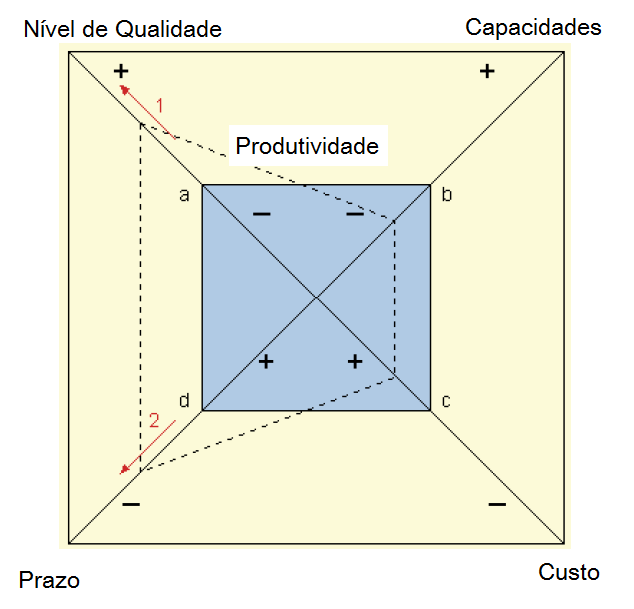
\includegraphics[scale=0.6]{devils_square.png}
 \caption{\label{fig:qpcs}\textit{The Devil's square}, adaptado de
 \cite{grunbacher2001surfacing} }
\end{figure*}
 
\FloatBarrier

A motivação deste trabalho é apresentar e comparar as técnicas de negociação de
requisitos, compilando todas as informações encontradas em um único
trabalho, visto que não encontramos nenhum com esta proposta, ainda que a
literatura sobre técnicas de negociação de requisitos seja ampla.
Entendemos que é de fundamental importância expor o conhecimento de forma
acessível, ou seja, fácil de se encontrar e de compreender, a fim de guiar os stakeholders
na sua busca por uma técnica adequada.

 \section{Objetivos}

Este trabalho visa apresentar um conjunto de técnicas de
negociação de requisitos encontradas na literatura, suas vantagens, suas
desvantagens e os achados importantes sobre cada uma. Para tal, buscamos realizar
uma revisão ampla, justa e quasi-sistemática da literatura.

\section{Organização da Monografia}

O restante deste trabalho está organizado da seguinte forma:
No Capítulo 2 descrevemos o planejamento, a execução e os dados extraídos da
revisão quasi-sistemática conduzida.
No capítulo 3 discutimos os resultados, respondendo as questãos de pesquisa.
Por fim, no capítulo 4 apresentamos as contribuições, limitações e perspectivas de trabalhos futuros.

\chapter{Raspberry PI}\label{cap:revisao}

Nesse capítulo serão apresentadas as ferramentas utilizados na implementação do projeto...

\section{Raspberry Pi 3 Versão B}

%% Falar das caracteristicas do hardware e sua comfiguração

\subsection{Motivação do uso do Raspberry}

%%Deixa essa comigo

\subsection{Métodos de instalação do Raspbian}

%%Falar sobre o noobs e a instalação direta em um passo-a-passo.

\subsection{Bitcoin Core}

%%Descrever os passos de compilação e instalação e mencionar a existencia do repositório apt-get no fim

O tipo de estudo mencionado acima, na QS2, provém da classificação apresentada
em \cite{wieringa2006requirements} e é descrita brevemente abaixo. Essas classes
foram usadas também em \cite{Kuhrmann:2015:SPI:2785592.2785600}.
  


Com essas indagações, pudemos construir e ajustar \textit{strings} de buscas de
forma que resultassem em possíveis respostas , até que chegássemos em uma
\textit{string} definitiva.


\begin{itemize}
\setlength{\itemsep}{1pt}
\setlength{\itemindent}{20pt}
\item {(("\textit{software}") AND ("\textit{scope}" OR
"\textit{requirements}") AND ("\textit{negotiation}"))}
\end{itemize}

A população (\textit{population}) da \textit{String} acima é definida por
'\textit{software}', '\textit{scope}' e '\textit{requirements}'; a intervenção (\textit{Intervention}) é definida como
'\textit{negotiation}'.
Não há na \textit{string} comparação (Comparison), já que não restringimos
nossos resultados aos artigos que comparem técnicas, como não há também uma definição
de resultados (Outcome), a fim de não haver nenhum tipo de restrição.

As próximas etapas deverão ser realizadas considerando os critérios de inclusão
e de exclusão. Definimos que se os pesquisadores discordarem sobre a
conformidade do artigo com esses critérios, um terceiro pesquisador faria também
uma avaliação. Esses critérios de inclusão e de exclusão são apresentados a
seguir.

Inclusão:
\begin{itemize}
\setlength{\itemsep}{1pt}
\setlength{\itemindent}{20pt}
\item {Artigos que descrevem, propõem, aplicam ou avaliam técnicas de negociação
de requisitos.}
\end{itemize}

Exclusão:
\begin{itemize}
\setlength{\itemsep}{1pt}
\setlength{\itemindent}{20pt}
\item {Artigos que não descrevem os passos de uma técnica de maneira
compreensível.}
\item {Artigos onde a técnica é somente mencionada.}
\item {Artigos em outros idiomas que não o inglês, para facilitar a reprodução
do protocolo em qualquer lugar do mundo.}
\item {Artigos que descrevem técnicas de negociação para contextos não presenciais (\textit{e.g.}, distribuídas).}
\end{itemize}

Para mensurar a eficiência de nossa \textit{String}, estipulamos alguns artigos
relevantes e que atendem as exigências impostas pelos critérios de inclusão,
exclusão e a definição do tema de pesquisa. Estes, chamados artigos de controle,
deveriam ser retornados como resultados da busca na biblioteca digital escolhida
e se encontram adiante.

\begin{enumerate}
\setlength{\itemsep}{1pt}
\setlength{\itemindent}{20pt}
\item \textit{software requirements negotiation using the software quality
function deployment \cite{ramires2005software}
  \item Integration of scrum with Win-Win requirements negotiation
  model \cite{khan2014integration}
\item Requirements Negotiation Using Multi-Criteria Preference
Analysis \cite{in2004requirements}}
\end{enumerate}

Os artigos resultantes da busca na biblioteca Scopus, seriam então analisados
por título e \textit{abstract}, levando em consideração o tema da pesquisa, os
critérios de inclusão e os critérios de exclusão.
Essa análise, naturalmente resultaria em dois conjuntos, o conjunto de artigos
aprovados e o conjunto de artigos reprovados. O primeiro destes, seria o ponto
de partida para a próxima etapa de filtragem, a filtragem por conteúdo.
Essa etapa consiste em os pesquisadores lerem cada artigo e avaliarem, segundo
os mesmos critérios já apresentados, se os artigos são ou não pertinentes para atingir o objetivo da pesquisa.
 Os artigos pertinentes serviriam como conjunto para a aplicação da técnica
 \textit{snowballing}, que contribui para a garantia da eficiência em encontrar
 artigos relevantes, sem perda de completude, quando comparada com buscar com a
 mesma \textit{String} em diferentes bibliotecas digitais
 \cite{Badampudi:2015:EUS:2745802.2745818}.
 
Com os artigos encontrados ao se aplicar o \textit{snowballing}, realizar-se-ia
a primeira e a segunda filtragem.
Este processo de filtragem e \textit{snowballing} é iterativo e possui como
condição de parada a não obtenção de novos resultados.

Com o conjunto final de todos os artigos, extrair-se-ão os dados a seguir.

\begin{itemize}
\setlength{
\itemsep}{1pt}
\setlength{
\itemindent}{20pt}
\item {Referência.}
\item {Nome da técnica.}
\item {Tem negociação de requisitos como alvo principal?}
\item {Descrição resumida da técnica (ou da parte referente à negociação de requisitos).}
\item {Ambiente (academia ou indústria).}
\item {Tipo de pesquisa (\textit{Evaluation research,
Solution proposal, Philosophical paper, Opinion paper, Experience paper)}.}
\item {Tipo de estudo primário (experimento, estudo de caso ou
\textit{survey}).}
\item {Achados principais do artigo (conhecimento gerado).}
\item {Vantagens.}
\item {Desvantagens.}
\end{itemize}

\section{Execução}

A \textit{string} de busca precisou ser adaptada para o formato da biblioteca
Scopus e o resultado dessa adaptação encontra-se a seguir.
 
 \begin{itemize}
\setlength{\itemsep}{1pt}
\setlength{\itemindent}{20pt}
\item {(("\textit{software}") AND ("\textit{scope}" OR "\textit{requirements}") AND ("negotiation" ))
AND ( LIMIT-TO(SUBJAREA,"COMP" ) OR LIMIT-TO(SUBJAREA,"ENGI" ) )}
\end{itemize}
 
A busca na biblioteca foi feita em 24 de novembro de 2015 e resultou em 408
artigos, que podem ser encontrados no apêndice. Esses, foram lidos e
filtrados como descrito no planejamento.
O conjunto obtido após a primeira filtragem continha 39 artigos e, após
a segunda filtragem restaram 18, que estão indicados no apêndice pela
cor cinza.

O segundo dos artigos de controle`, \cite{khan2014integration}, não havia sido
capturado devido a restrição por área (computação e engenharia), que foi posta,
a fim de que resultados de administração e economia, por exemplo, não fossem retornados. O motivo
para o artigo de controle não ter sido um dos resultados foi que o mesmo havia
sido cadastrado como 'multiarea'. A forma que foi indexado não é de nossa
compreensão, contudo entendemos que foi uma falha, visto que o mesmo é
claramente da área de computação. Este, então, também teve seus dados extraídos
e está contido nos 18 artigos mencionados.

 A busca na base Scopus permitiu obter de forma imparcial um conjunto de artigos que pudesse ser utilizado
 como \textit{seed set} para dar início ao \textit{backward snowballing}, que
 consiste em capturar todas as referências encontradas para cada um dos artigos
 do \textit{seed set}. O número total de referências foi de 383. Realizamos
 então a filtragem por título e, sendo assim, restaram 96, que continham
 duplicadas e removendo-as restaram 56. A filtragem por abstract reduziu o número à 26, entretanto desses somente 21 foram encontrados para filtragem por conteúdo e, esta última filtragem resultou em 15 artigos válidos,
que tiveram suas informações extraídas.

A Figura 2.1 representa como os artigos do
\textit{seed set} se relacionam em termos de citeções, enquanto a figura 2.2
mostra como todos os artigos encontrados estão relacionados em termos de
citações, sejam eles do \textit{seed set} ou provenientes do \textit{backward
snowballing}.

\begin{figure}[ht]
 \centering
 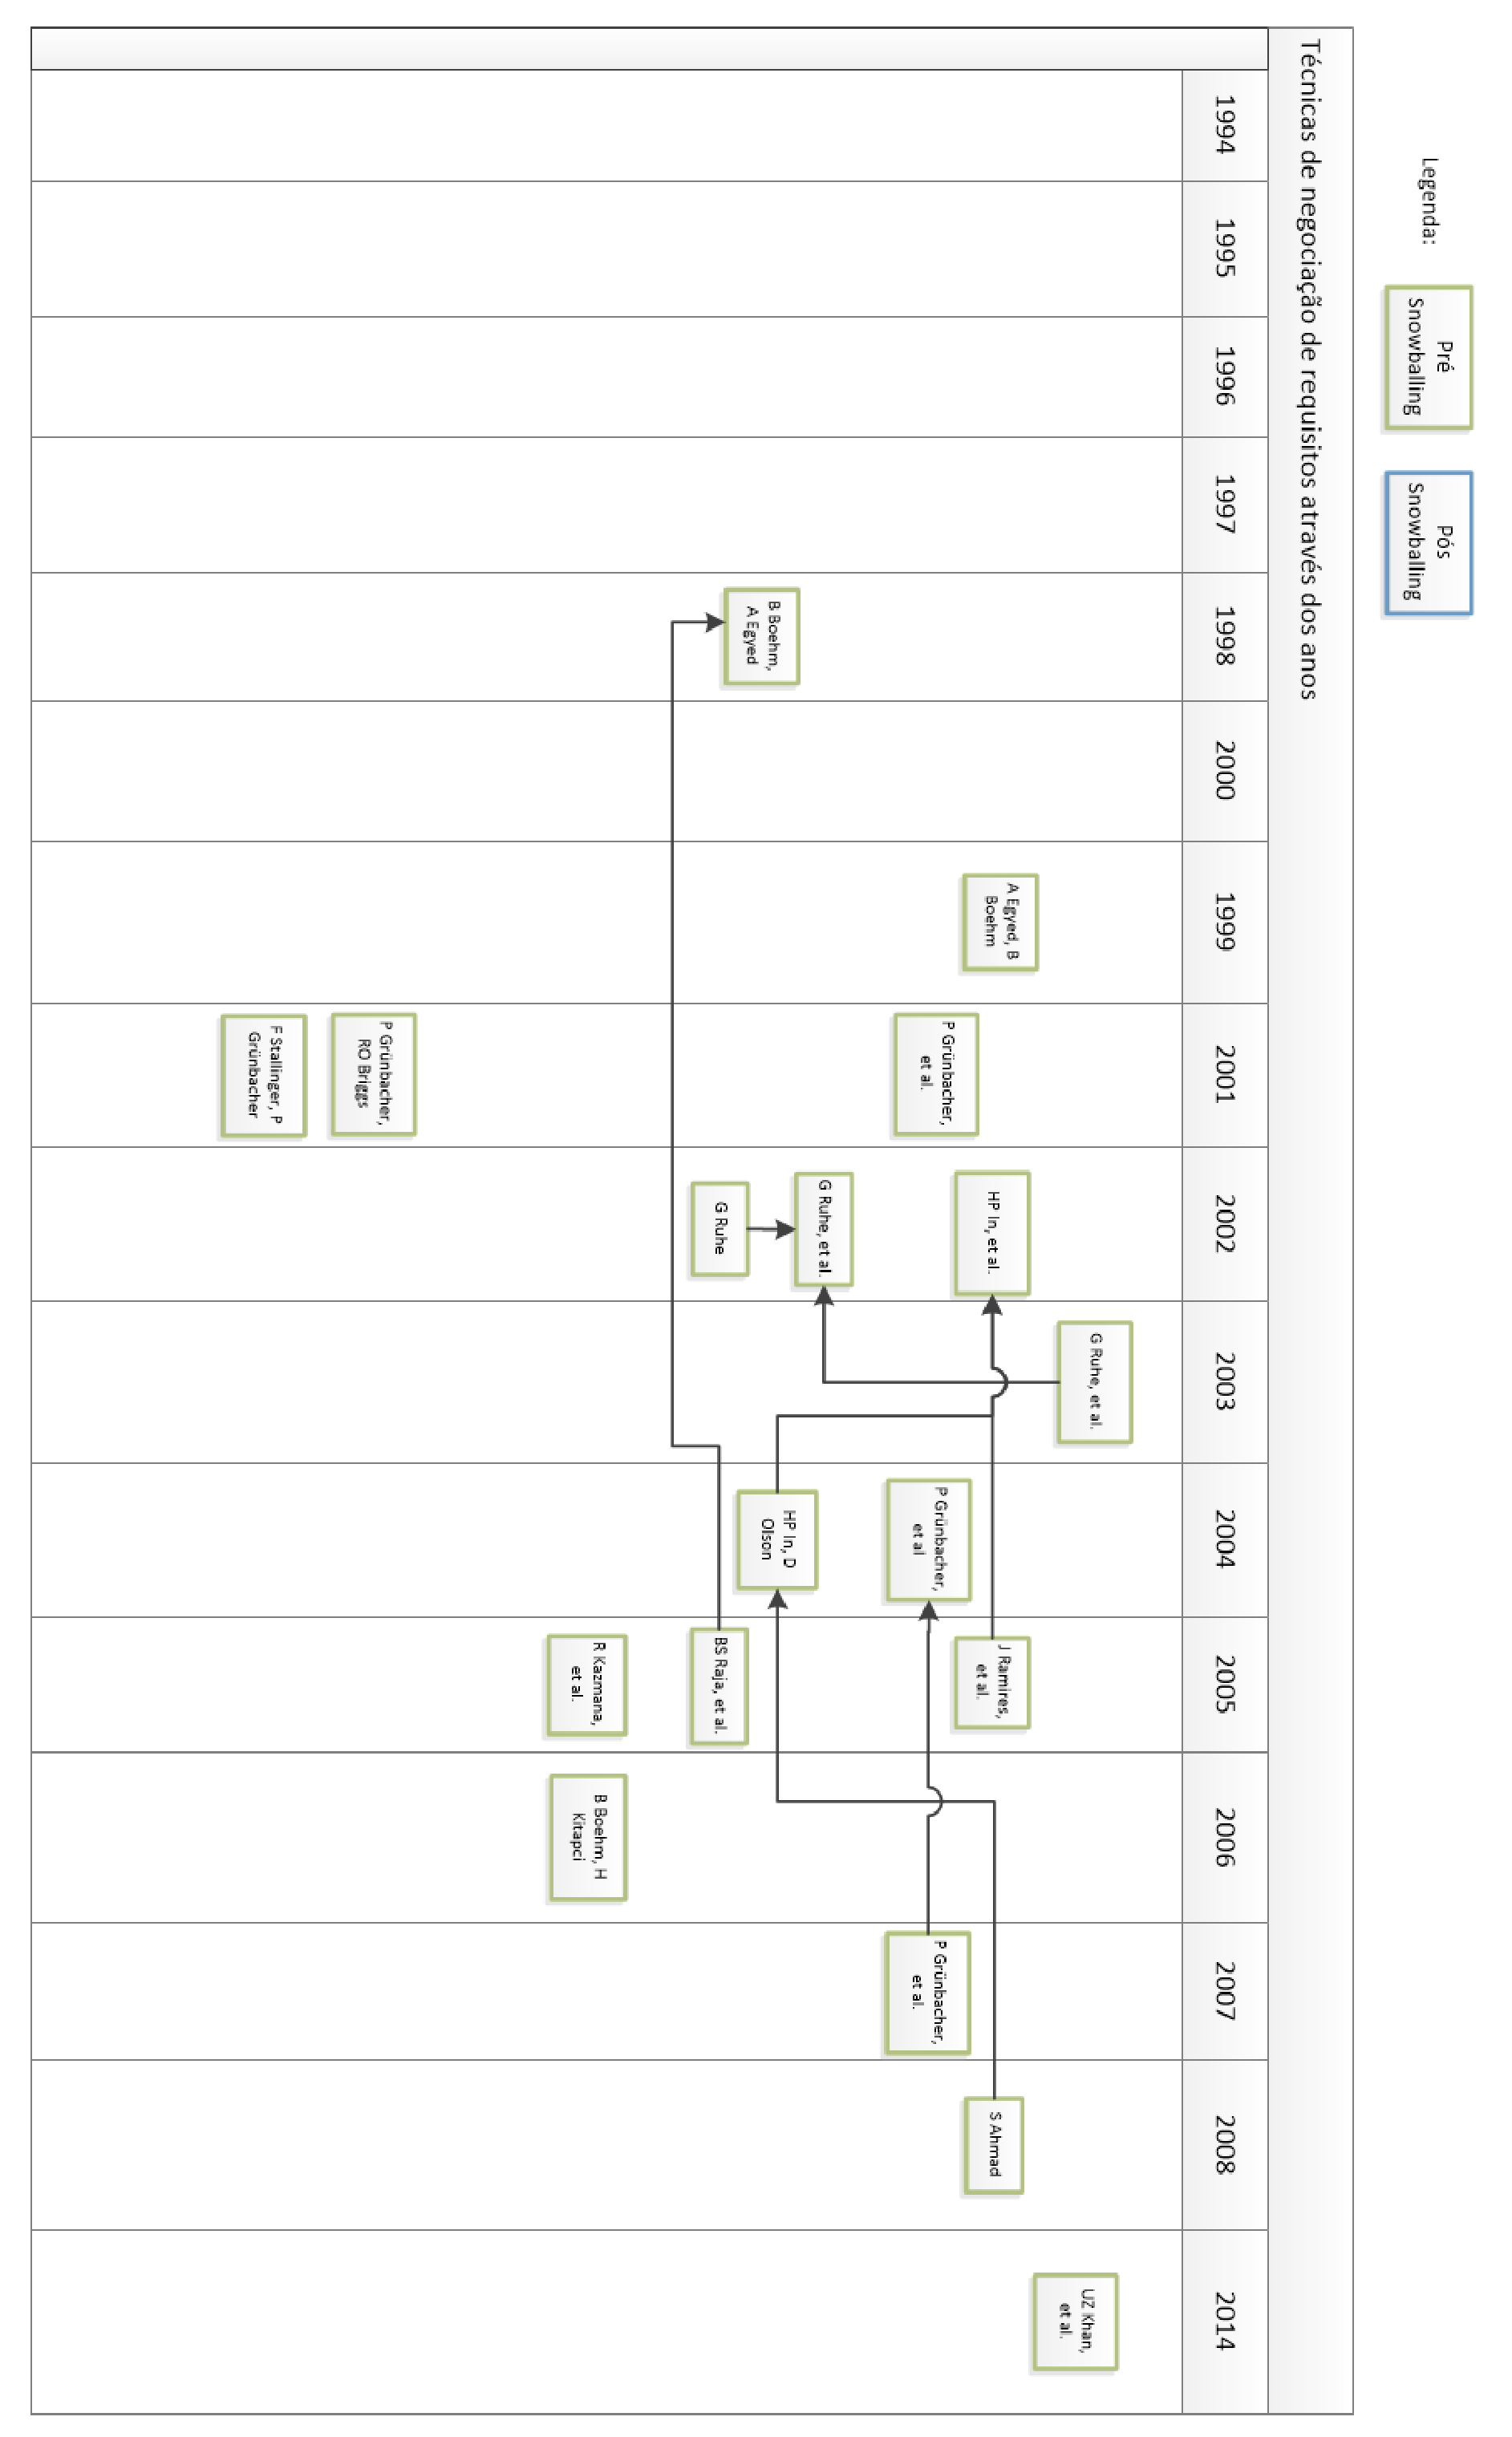
\includegraphics[scale=0.47]{pre_sb.eps}
 \caption{\label{fig:presb}Diagrama de Citações Pré \textit{Backward
 Snowballing}}
\end{figure}

\FloatBarrier

\begin{figure}[ht]
 \centering
 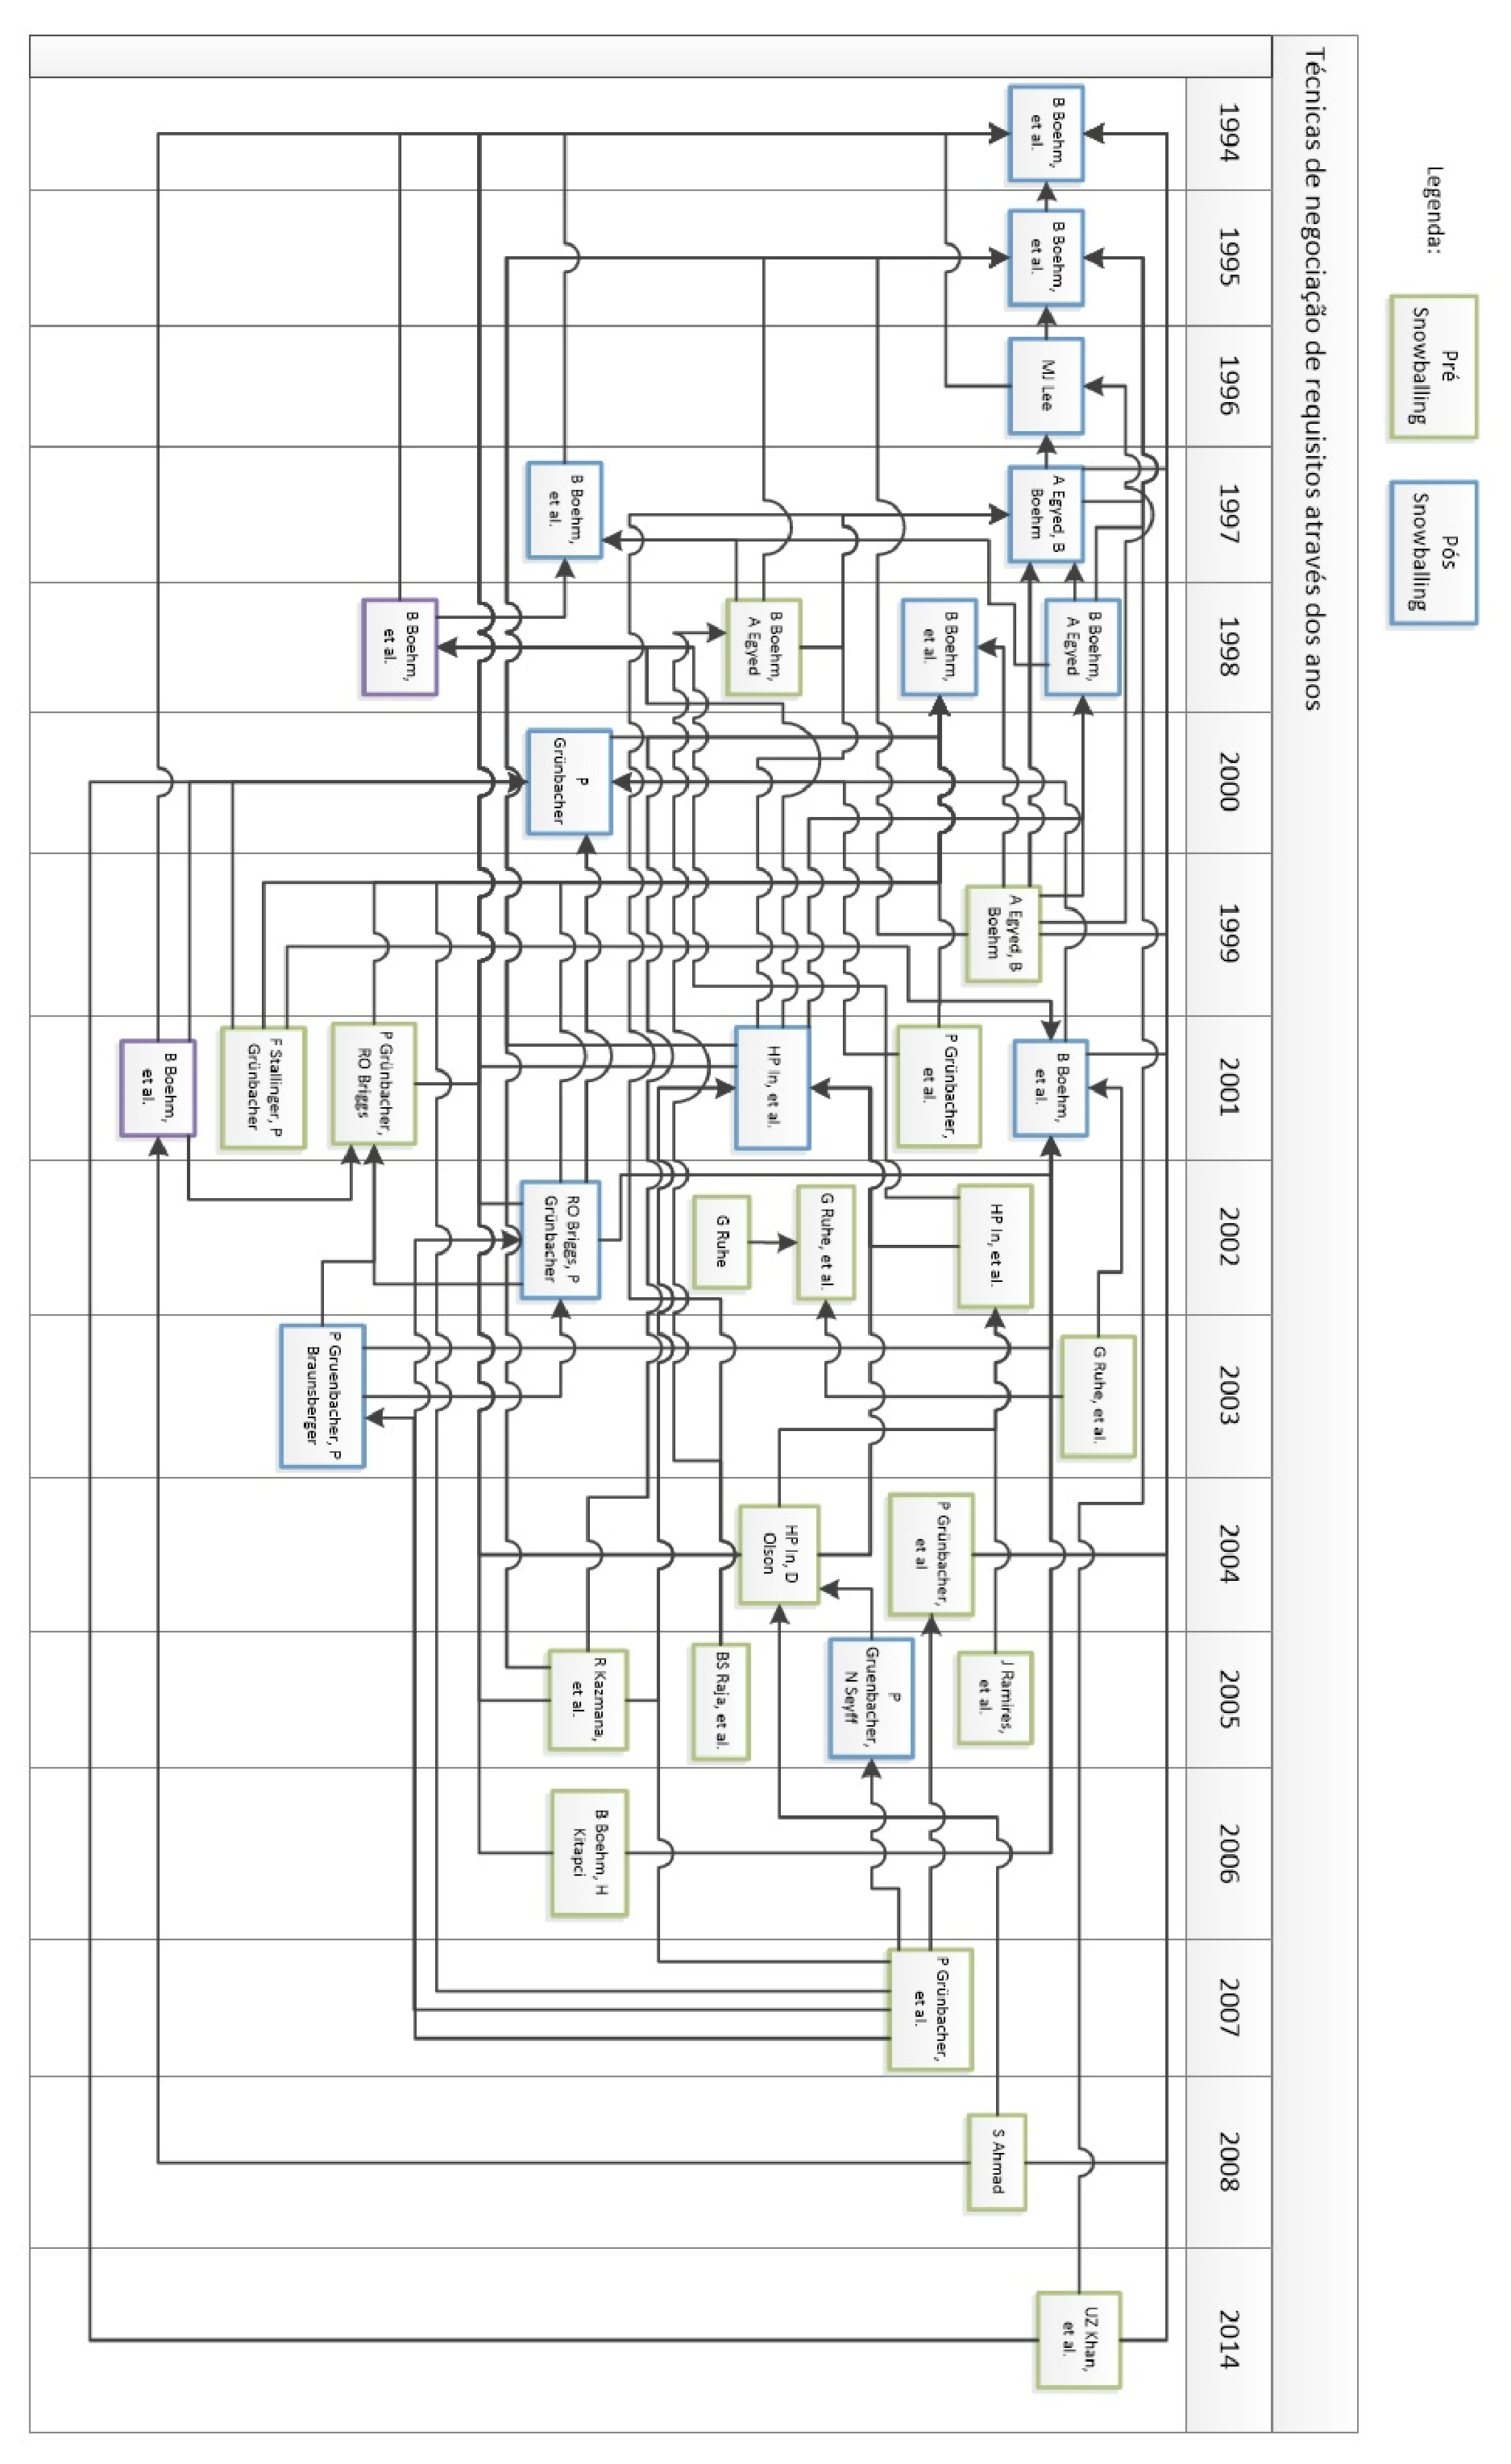
\includegraphics[scale=0.48]{final_sb.eps}
 \caption{\label{fig:possb}Diagrama de Citações pós \textit{Backward
 Snowballing}}
\end{figure}

\FloatBarrier

\section{Dados Extraídos}

Esta seção tem como objetivo apresentar os dados extraídos para cada um dos 33
artigos encontrados após a execução do protocolo da revisão quasi-sistemática.
Esses dados foram agrupados e debatidos para que pudéssemos responder as
questões de pesquisa, que foram apresentadas na seção do planejamento deste capítulo.
Essas respostas serão apresentadas no capítulo 3.


\begin{longtable}{{|>{\centering\arraybackslash}m{3cm}|>{\centering\arraybackslash}m{10cm}|}}
\caption{\label{fig:t1}Comparing software system requirements negotiation
patterns. Systems Engineering}\\
\hline 
\textbf{Referência}                                         & EGYED, Alexander;
BOEHM, Barry. \textit{Comparing software system requirements negotiation
patterns.}
\textit{Systems Engineering}, v. 2, n. 1, p. 1-14, 1999.
\cite{egyed1999comparing} \\ \hline \textbf{Nome da técnica}                                    & \textit{WinWIn}                    \\
\hline
\textbf{O foco é a negociação de requisitos?}               & Sim                       \\
\hline
\textbf{Descrição da técnica}                               & I                        \\
\hline
\textbf{Ambiente}                                           & Academia/indústria         \\
\hline
\textbf{Tipo de pesquisa}                                   & \textit{Evaluation
research}        \\
\hline
\textbf{Tipo de estudo primário (quando houver)}            & estudo de caso             \\
\hline
\textbf{Achados Principais do Artigo (Conhecimento Gerado)} & Foi verificado que clientes e usuários são mais presentes na etapa de identificação das condições de vitória, enquanto os desenvolvedores foram mais presentes na definição de problemas e nas suas opções de resolução. \\ \hline
\textbf{Vantagens}                                          &                          \\
\hline
\textbf{Desvantagens}                                       &                          \\
\hline

\end{longtable}

\begin{longtable}{{|>{\centering\arraybackslash}m{3cm}|>{\centering\arraybackslash}m{10cm}|}}
\caption{\label{fig:t2}Making every student a winner: The WinWin approach in
software engineering education.}\\
\hline 
\textbf{Referência}                                         & GRÜNBACHER, Paul
et al. Making every student a winner: The WinWin approach in software
engineering education. Journal of Systems and software, v. 80, n. 8, p.
1191-1200, 2007. \cite{grunbacher2007making} \\ \hline \textbf{Nome da técnica}                          
& \textit{WinWIn}                                                                                                                                                                          \\ \hline \textbf{O foco é a negociação de requisitos?}               & Sim                                                                                                                                                                             \\ \hline \textbf{Descrição da técnica}                               & I                                                                                                                                                                               \\ \hline \textbf{Ambiente}                                           & Academia                                                                                                                                                                        \\ \hline
\textbf{Tipo de pesquisa}                                   & \textit{Solution proposal}                                                                                                                                                                \\ \hline
\textbf{Tipo de estudo primário (quando houver)}            & Estudo de caso                                                                                                                                                              \\ \hline
\textbf{Achados Principais do Artigo (Conhecimento Gerado)} & Os alunos se sentem mais motivados a participar quando existe um papel de facilitador.                                                                                          \\ \hline
\textbf{Vantagens}                                          & Estimula a comunicação, ajuda na reconciliação de pontos conflitantes, ajuda na identificação de problemas e incertezas, tal como na percepção de possíveis acordos.            \\ \hline
\textbf{Desvantagens}                                       & Foi mencionado em quase todos os relatos que era preciso mais tempo para ensinar a metodologia.                                                                                 \\ \hline

\end{longtable}


\begin{longtable}{{|>{\centering\arraybackslash}m{3cm}|>{\centering\arraybackslash}m{10cm}|}}
\caption{\label{fig:t3}Quantitative WinWin: a new method for decision support in
requirements negotiation}\\
\hline
\textbf{Referência}                                         & RUHE, Günther;
EBERLEIN, Armin; PFAHL, Dietmar. Quantitative WinWin: a new method for decision
support in requirements negotiation. In: Proceedings of the 14th international
conference on software engineering and knowledge engineering. ACM, 2002. p.
159-166. \cite{ruhe2002quantitative}                                            
\\ \hline \textbf{Nome da técnica}                                    &
\textit{Quantitative WinWin}                                                    
\\ \hline \textbf{O foco é a negociação de requisitos?}               & Sim                                                                                                                                                                                                                                                                                                                   \\ \hline \textbf{Descrição da técnica}                               & II                                                                                                                                                                                                                                                                                                                     \\ \hline \textbf{Ambiente}                                           & Academia                                                                                                                                                                                                                                                                                                              \\ \hline \textbf{Tipo de pesquisa}                                   & \textit{Solution proposal}                                                                                                                                                                                                                                                                                                     \\ \hline \textbf{Tipo de estudo primário (quando houver)}            & Estudo de caso                                                                                                                                                                                                                                                                                                        \\ \hline \textbf{Achados Principais do Artigo (Conhecimento Gerado)} &                                                                                                                                                                                                                                                                                                                       \\ \hline
\textbf{Vantagens}                                          & A técnica não se
baseia em questões subjetivas para sua tomada de decisão como se faz na
\textit{WinWin}. Muito pelo contrário, ela se utiliza de dados quantitativos para basear melhor sua tomada de decisão.                                                                                                                \\ \hline \textbf{Desvantagens}                                       & Foi feita apenas uma simulação utilizando dados da indústria, logo não há confirmação real de que a técnica funcionaria corretamente em situações maiores e mais complexas. Ela também necessita de uma estimativa bastante efetiva e precisa do esforço atrelado a cada requisito para que sua análise seja efetiva. \\ \hline

\end{longtable}



\begin{longtable}{{|>{\centering\arraybackslash}m{3cm}|>{\centering\arraybackslash}m{10cm}|}}
\caption{\label{fig:t4}Requirements Negotiation Using Multi-Criteria Preference Analysis}\\
\hline
\textbf{Referência}                                         & IN, Hoh Peter;
OLSON, David. Requirements Negotiation Using Multi-Criteria Preference Analysis.
J. UCS, v. 10, n. 4, p. 306-325, 2004. \cite{in2004requirements}                                      
\\ \hline \textbf{Nome da técnica}                                    & MPARN                                                                                                                                                                                                  \\ \hline \textbf{O foco é a negociação de requisitos?}               & Sim                                                                                                                                                                                                    \\ \hline \textbf{Descrição da técnica}                               & III                 
\\ \hline \textbf{Ambiente}                                           & Academia                                                                                                                                                                                               \\ \hline
\textbf{Tipo de pesquisa}                                   & \textit{Solution proposal}                                                                                                                                                                                      \\ \hline
\textbf{Tipo de estudo primário (quando houver)}            & Estudo de caso                                                                                                                                                                                         \\ \hline
\textbf{Achados Principais do Artigo (Conhecimento Gerado)} &                                                                                                                                                                                                        \\ \hline
\textbf{Vantagens}                                          & Análise de opções menos subjetiva e mais objetiva.                                                                                                                                                     \\ \hline
\textbf{Desvantagens}                                       & Não possui boa
solução para sistema de como se tomar a decisão final. Não foi feito nenhum experimento concreto sobre a eficácia da técnica, estudo de caso detalhado no artigo era hipotético. \\ \hline

\end{longtable}


\begin{longtable}{{|>{\centering\arraybackslash}m{3cm}|>{\centering\arraybackslash}m{10cm}|}}
\caption{\label{fig:t5}Multi-criteria preference analysis for systematic
requirements negotiation}\\
\hline
\textbf{Referência}                                         & IN, Hoh Peter;
OLSON, David; RODGERS, Tom. Multi-criteria preference analysis for systematic
requirements negotiation. In: Computer software and Applications Conference,
2002. COMPSAC 2002. Proceedings. 26th Annual International. IEEE, 2002. p.
887-892.  \cite{in2002multi}                                                                 
\\ \hline \textbf{Nome da técnica}                                    & MPARN                                                                                                                                                                                                                                                                                                                                                                                                                                                                                                                                                                                        \\ \hline \textbf{O foco é a negociação de requisitos?}               & Sim                                                                                                                                                                                                                                                                                                                                                                                                                                                                                                                                                                                          \\ \hline \textbf{Descrição da técnica}                               & III \\ \hline \textbf{Ambiente}                                           & Academia                                                                                                                                                                                                                                                                                                                                                                                                                                                                                                                                                                                     \\ \hline \textbf{Tipo de pesquisa}                                   & \textit{Solution proposal}                                                                                                                                                                                                                                                                                                                                                                                                                                                                                                                                                                          \\ \hline
\textbf{Tipo de estudo primário (quando houver)}            & estudo de caso                                                                                                                                                                                                                                                                                                                                                                                                                                                                                                                                                                               \\ \hline
\textbf{Achados Principais do Artigo (Conhecimento Gerado)} & Existem algumas
maneiras de guiar alguns dos passos apresentados no MPARN, por exemplo: No passo
5 pode-se usar um método direto, método com função linear, método com função não linear, método com progressão geométrica, existem,outros métodos não abordados no artigo. No passo 6: pode se usar um método subjetivo direto, método smart, método de comparação de razão em pares, método com progressão geométrica,ou outro que não foi dito no artigo. No passo 7: pode se usar forma democrática, democrática por meios aritméticos, democrática por meios geométricos ou ditatorial. \\ \hline \textbf{Vantagens}                                          &                                                                                                                                                                                                                                                                                                                                                                                                                                                                                                                                                                                              \\ \hline \textbf{Desvantagens}                                                                                                                                                                       &                                                                                                                                                                                                                                                               \\ \hline

\end{longtable}
\begin{longtable}{{|>{\centering\arraybackslash}m{3cm}|>{\centering\arraybackslash}m{10cm}|}}
\caption{\label{fig:t6}From requirements negotiation to software architecture
decisions}\\
\hline
\textbf{Referência}                                         & KAZMAN, Rick; IN,
Hoh Peter; CHEN, Hong-Mei. From requirements negotiation to software
architecture decisions. Information and software Technology, v. 47, n. 8, p.
511-520, 2005.  \cite{kazman2005requirements}                                                            
\\ \hline \textbf{Nome da técnica}                                    & Win CBAM                                                                                                                                                                                                                                                                                                                                                                                                                                   \\ \hline \textbf{O foco é a negociação de requisitos?}               & Sim                                                                                                                                                                                                                                                                                                                                                                                                                                        \\ \hline \textbf{Descrição da técnica}                               & IV \\ \hline \textbf{Ambiente}                                           & Academia/indústria                                                                                                                                                                                                                                                                                                                                                                                                                         \\ \hline
\textbf{Tipo de pesquisa}                                   & \textit{Evaluation research}                                                                                                                                                                                                                                                                                                                                                                                                                        \\ \hline
\textbf{Tipo de estudo primário (quando houver)}            & Estudo de caso                                                                                                                                                                                                                                                                                                                                                                                                                             \\ \hline
\textbf{Achados Principais do Artigo (Conhecimento Gerado)} &                                                                                                                                                                                                                                                                                                                                                                                                                                            \\ \hline
\textbf{Vantagens}                                          & A técnica captura
erro da quantificação pelos \textit{stakeholders} na etapa 5. A técnica agrega
valor não só na negociação de atributos de qualidade e de estratégias de arquitetura, mas
também consegue fornecer uma forma dos \textit{stakeholders} perceberem a ligação das
estratégias de arquitetura e dos atributos de qualidade com os requisitos,
possibilitando que os \textit{stakeholders} possam repensar os requisitos sob uma nova
perspectiva. \\ \hline \textbf{Desvantagens}                                    
& A técnica não apresenta forma de calcular o custo, pois supõe que a empresa já
adote alguma metodologia para isso                                                                                                                                                                                                                                                                                                                          \\ \hline
\end{longtable}



\begin{longtable}{{|>{\centering\arraybackslash}m{3cm}|>{\centering\arraybackslash}m{10cm}|}}
\caption{\label{fig:t7}The WinWin approach: using a requirements negotiation tool for rationale capture and use}\\
\hline
\textbf{Referência}                                         & BOEHM, Barry;
KITAPCI, Hasan. The WinWin approach: using a requirements negotiation tool for
rationale capture and use. In: Rationale management in software engineering.
Springer Berlin Heidelberg, 2006. p. 173-190. \cite{boehm2006winwin}                              
\\ \hline \textbf{Nome da técnica}                                    & \textit{WinWIn}                                                                                                                                                                                                                                                           \\ \hline \textbf{O foco é a negociação de requisitos?}               & Sim                                                                                                                                                                                                                                                              \\ \hline \textbf{Descrição da técnica}                               & I                                                                                                                                                                                                                                                                \\ \hline \textbf{Ambiente}                                           & Academia/indústria                                                                                                                                                                                                                                               \\ \hline
\textbf{Tipo de pesquisa}                                   & \textit{Experience paper}                                                                                                                                                                                                                                                 \\ \hline
\textbf{Tipo de estudo primário (quando houver)}            & Experimento                                                                                                                                                                                                                                                      \\ \hline
\textbf{Achados Principais do Artigo (Conhecimento Gerado)} & A equipe que usou o \textit{WinWIn} foi capaz de gerar resultados mais amplos e profundos. O \textit{WinWIn} também serve como forma de se documentar a tomada de decisão na negociação de requisitos.                                                                             \\ \hline
\textbf{Vantagens}                                          & A ferramenta EasyWinWin facilita a transição entre negociação de requisitos e especificação de requisitos.                                                                                                                                                       \\ \hline
\textbf{Desvantagens}                                       & A especificação de
requisitos gerada após o \textit{WinWIn}, tipicamente não é completa, precisa,
consistente e testável, pois vários dos requisitos podem ter sido permitidos durante a empolgação dos \textit{stakeholders} com o alto nível de cooperação durante a negociação. \\ \hline

\end{longtable}


\begin{longtable}{{|>{\centering\arraybackslash}m{3cm}|>{\centering\arraybackslash}m{10cm}|}}
\caption{\label{fig:t8}Trade-off analysis for requirements selection}\\
\hline
\textbf{Referência}                                         & RUHE, Günther;
EBERLEIN, Armin; PFAHL, Dietmar. Trade-off analysis for requirements selection.
International Journal of software Engineering and Knowledge Engineering, v. 13,
n. 04, p. 345-366, 2003. \cite{ruhe2003trade}                                                   
\\ \hline \textbf{Nome da técnica}                                    & \textit{Quantitative WinWin}                                                                                                                                                                                                                                                                                                   \\ \hline \textbf{O foco é a negociação de requisitos?}               & Sim                                                                                                                                                                                                                                                                                                                   \\ \hline \textbf{Descrição da técnica}                               & II                                                                                                                                                                                                                                                                                                                     \\ \hline \textbf{Ambiente}                                           & Academia                                                                                                                                                                                                                                                                                                              \\ \hline
\textbf{Tipo de pesquisa}                                   & \textit{Solution proposal}                                                                                                                                                                                                                                                                                                     \\ \hline
\textbf{Tipo de estudo primário (quando houver)}            & Experimento                                                                                                                                                                                                                                                                                                           \\ \hline
\textbf{Achados Principais do Artigo (Conhecimento Gerado)} &                                                                                                                                                                                                                                                                                                                       \\ \hline
\textbf{Vantagens}                                          & A técnica não se baseia em questões subjetivas para sua tomada de decisão como se faz na \textit{WinWIn}. Muito pelo contrário, ela se utiliza de dados quantitativos para basear melhor sua tomada de decisão.                                                                                                                \\ \hline
\textbf{Desvantagens}                                       & Foi feita apenas uma simulação utilizando dados da indústria, logo não há confirmação real de que a técnica funcionaria corretamente em situações maiores e mais complexas. Ela também necessita de uma estimativa bastante efetiva e precisa do esforço atrelado a cada requisito para que sua análise seja efetiva. \\ \hline

\end{longtable}

\begin{longtable}{{|>{\centering\arraybackslash}m{3cm}|>{\centering\arraybackslash}m{10cm}|}}
\caption{\label{fig:t9}Negotiation in the requirements elicitation and analysis process}\\
\hline
\textbf{Referência}                                         & AHMAD, Sabrina.
Negotiation in the requirements elicitation and analysis process. In: 19th
Australian Conference on software Engineering (aswec 2008). IEEE, 2008. p.
683-689. \cite{ahmad2008negotiation} \\ \hline \textbf{Nome da técnica}                                   
& Requirement Negotiation Spiral Model                                                                                                                                           \\ \hline \textbf{O foco é a negociação de requisitos?}               & Sim                                                                                                                                                                            \\ \hline \textbf{Descrição da técnica}                               & V \\ \hline \textbf{Ambiente}                                           & Academia                                                                                                                                                                       \\ \hline
\textbf{Tipo de pesquisa}                                   & \textit{Solution proposal}                                                                                                                                                              \\ \hline
\textbf{Tipo de estudo primário (quando houver)}            &                                                                                                                                                                                \\ \hline
\textbf{Achados Principais do Artigo (Conhecimento Gerado)} &                                                                                                                                                                                \\ \hline
\textbf{Vantagens}                                          &                                                                                                                                                                                \\ \hline
\textbf{Desvantagens}                                       &                                                                                                                                                                                \\ \hline

\end{longtable}


% Please add the following required packages to your document preamble:
% \usepackage[normalem]{ulem}
% \useunder{\uline}{\ul}{}
\begin{longtable}{{|>{\centering\arraybackslash}m{3cm}|>{\centering\arraybackslash}m{10cm}|}}
\caption{\label{fig:t10}Integrating collaborative processes and quality
assurance techniques: experiences from requirements negotiation}\\
\hline
\textbf{Referência}                                         & GRÜNBACHER, Paul
et al. Integrating collaborative processes and quality assurance techniques:
experiences from requirements negotiation. Journal of Management Information
Systems, v. 20, n. 4, p. 10-30, 2004. \cite{grunbacher2004integrating}                                        
\\ \hline \textbf{Nome da técnica}                                    & QA EasyWinWin                                                                                                                                                                                                                                                                                                                                                                                                                                                                                                                                                                                                                                                                                                                                                                                \\ \hline \textbf{O foco é a negociação de requisitos?}               & Sim                                                                                                                                                                                                                                                                                                                                                                                                                                                                                                                                                                                                                                                                                                                                                                                          \\ \hline \textbf{Descrição da técnica}                               & VI \\ \hline \textbf{Ambiente}                                           & Academia                                                                                                                                                                                                                                                                                                                                                                                                                                                                                                                                                                                                                                                                                                                                                                                     \\ \hline
\textbf{Tipo de pesquisa}                                   & \textit{Evaluation research}                                                                                                                                                                                                                                                                                                                                                                                                                                                                                                                                                                                                                                                                                                                                                                            \\ \hline
\textbf{Tipo de estudo primário (quando houver)}            & Experimento                                                                                                                                                                                                                                                                                                                                                                                                                                                                                                                                                                                                                                                                                                                                                                                  \\ \hline
\textbf{Achados Principais do Artigo (Conhecimento Gerado)} & Achados dizem
respeito apenas a fase pós negociação. Os inspetores acharam útil o modelo do
Easy \textit{WinWIn} para negociação e documentação de requisitos. Maior detalhamento na
documentação dos requisitos facilita a aplicação do Easy WinWin. Houve um
consenso entre os envolvidos que as técnicas de inspeção e de leitura se
encaixaram bem com os artefatos a serem inspecionados, e que os resultados do
Easy \textit{WinWIn} foram melhorados consideravelmente com a inspeção. O fato de a
técnica de detecção de defeitos destacar rapidamente os,defeitos relevantes do
ponto de vista de um \textit{stakeholder}, faz com que defeitos em geral possam passar
desapercebidos. Alguns inspetores argumentaram que a técnica de leitura era
ineficiente quando usada em artefatos pequenos e/ou simples. \\ \hline \textbf{Vantagens}                                          & Resultado final com menos erros.                                                                                                                                                                                                                                                                                                                                                                                                                                                                                                                                                                                                                                                                                                                                                             \\ \hline \textbf{Desvantagens}                                       &                                                                                                                                                                                                                                                                                                                                                                                                                                                                                                                                                                                                                                                                                                                                                                                              \\ \hline

\end{longtable}


\begin{longtable}{{|>{\centering\arraybackslash}m{3cm}|>{\centering\arraybackslash}m{10cm}|}}
\caption{\label{fig:t11}Reconciling software requirements and architectures: The
cbsp approach}\\
\hline
\textbf{Referência}                                                             
& GRUNBACHER, Paul; EGYED, Alexander; MEDVIDOVIC, Nenad. Reconciling software
requirements and architectures: The cbsp approach. In: Requirements Engineering,
2001. Proceedings. Fifth IEEE International Symposium on. IEEE, 2001. p.
202-211. \cite{grunbacher2001reconciling} 
\\  \hline \textbf{Nome da técnica}                                 
& CBSP                                                                                                                                                                                                                                           \\ \hline \textbf{O foco é a negociação de requisitos?}                                       & Sim                                                                                                                                                                                                                                            \\ \hline
\textbf{Descrição da técnica}                                                   
& VII                                                                         
\\ \hline \textbf{Ambiente}                                                                   & Indústria                                                                                                                                                                                                                                      \\ \hline \textbf{Tipo de pesquisa}                                                           & \textit{Evaluation research}                                                                                                                                                                                                                            \\ \hline
\textbf{Tipo de estudo primário (quando houver)}                                    & Estudo de caso                                                                                                                                                                                                                                 \\ \hline
\textbf{Achados Principais do Artigo (Conhecimento Gerado)}                         &                                                                                                                                                                                                                                                \\ \hline
\textbf{Vantagens}                                                                  & Existe um apoio numérico para a tomada de decisão ao se utilizar o coeficiente de concordância de ""Kendall. A técnica não se restringe a domínios bem específicos e é bem abrangente.  \\ \hline
\textbf{Desvantagens}                                                               &                                                                                                                                                                                                                                                \\ \hline

\end{longtable}

\begin{longtable}{{|>{\centering\arraybackslash}m{3cm}|>{\centering\arraybackslash}m{10cm}|}}
\caption{\label{fig:t12}Surfacing tacit knowledge in requirements negotiation:
experiences using EasyWinWin}\\
\hline
\textbf{Referência}                                         & GRUNBACHER, P.;
BRIGGS, Robert O. Surfacing tacit knowledge in requirements negotiation:
experiences using EasyWinWin. In: System Sciences, 2001. Proceedings of the 34th
Annual Hawaii International Conference on. IEEE, 2001. p. 8 pp.
\cite{grunbacher2001surfacing}  \\
\hline \textbf{Nome da técnica}                                    & Easy WinWin                                                                                                                                                                                                                               \\ \hline \textbf{O foco é a negociação de requisitos?}               & Sim                                                                                                                                                                                                                                       \\ \hline \textbf{Descrição da técnica}                               & 11                                                                                                                                                                                                                                        \\ \hline \textbf{Ambiente}                                           & Academia                                                                                                                                                                                                                                  \\ \hline
\textbf{Tipo de pesquisa}                                   & \textit{Solution proposal}                                                                                                                                                                                                                       \\ \hline
\textbf{Tipo de estudo primário (quando houver)}            & Estudo de caso                                                                                                                                                                                                                            \\ \hline
\textbf{Achados Principais do Artigo (Conhecimento Gerado)} & "-em uma reunião de 1 hora, com 10 \textit{stakeholders} são geradas em média 300 condições de vitórias. -de 1/3 à 1/2 das condições de vitórias são definidas em brainstormings.                                                                  \\ \hline
\textbf{Vantagens}                                          & -O conhecimento é gerado de forma colaborativa, o que permite alinhar expectativas e informações gerais.                                                                                                                                  \\ \hline
\textbf{Desvantagens}                                       &                                                                                                                                                                                                                                           \\ \hline

\end{longtable}


\begin{longtable}{{|>{\centering\arraybackslash}m{3cm}|>{\centering\arraybackslash}m{10cm}|}}
\caption{\label{fig:t13} System dynamics modelling and simulation of
collaborative requirements engineering}\\
\hline
\textbf{Referência}                                         & STALLINGER,
Friedrich; GRÜNBACHER, Paul. System dynamics modelling and simulation of
collaborative requirements engineering. Journal of Systems and software, v. 59,
n. 3, p. 311-321, 2001. \cite{stallinger2001system} \\ \hline \textbf{Nome da
técnica} & Easy WinWin                                                                                                                                                                                  \\ \hline \textbf{O foco é a negociação de requisitos?}               & Sim                                                                                                                                                                                          \\ \hline \textbf{Descrição da técnica}                               & VIII \\ \hline \textbf{Ambiente}                                           & Academia                                                                                                                                                                                     \\ \hline
\textbf{Tipo de pesquisa}                                   & \textit{Experience paper}                                                                                                                                                                             \\ \hline
\textbf{Tipo de estudo primário (quando houver)}            &                                                                                                                                                                                              \\ \hline
\textbf{Achados Principais do Artigo (Conhecimento Gerado)} & uso de categorias para as prioridades, mediante sua importância e viabilidade.                                                                                                               \\ \hline
\textbf{Vantagens}                                          &                                                                                                                                                                                              \\ \hline
\textbf{Desvantagens}                                       &                                                                                                                                                                                              \\ \hline

\end{longtable}


\begin{longtable}{{|>{\centering\arraybackslash}m{3cm}|>{\centering\arraybackslash}m{10cm}|}}
\caption{\label{fig:t14}software requirements negotiation: some lessons
learned}\\
\hline
\textbf{Referência}                                         & BOEHM, Barry;
EGYED, Alexander. software requirements negotiation: some lessons learned. In:
software Engineering, 1998. Proceedings of the 1998 International Conference on.
IEEE, 1998. p. 503-506. \cite{boehm1998software}                                                    
\\ \hline \textbf{Nome da técnica}                                    & \textit{WinWIn}                                                                                                                                                                                                                                                                                                                                                                                      \\ \hline \textbf{O foco é a negociação de requisitos?}               & Sim                                                                                                                                                                                                                                                                                                                                                                                         \\ \hline \textbf{Descrição da técnica}                               & 1                                                                                                                                                                                                                                                                                                                                                                                           \\ \hline \textbf{Ambiente}                                           & Academia                                                                                                                                                                                                                                                                                                                                                                                    \\ \hline
\textbf{Tipo de pesquisa}                                   & \textit{Experience paper}                                                                                                                                                                                                                                                                                                                                                                              \\ \hline
\textbf{Tipo de estudo primário (quando houver)}            &                                                                                                                                                                                                                                                                                                                                                                               \\ \hline
\textbf{Achados Principais do Artigo (Conhecimento Gerado)} & Tempo de duração não se correlaciona, necessariamente, com qualidade, porém esforço de negociar se relaciona. Pouca experiência e pouco esforço, resultaram em baixa qualidade. Usuários e clientes eram mais ativos no início, enquanto desenvolvedores e clientes nos estágios finais. Processo iterativo teve nota de lco bem maior que, quando usado processo em cascata de negociação. \\ \hline
\textbf{Vantagens}                                          &                                                                                                                                                                                                                                                                                                                                                                                             \\ \hline
\textbf{Desvantagens}                                       &                                                                                                                                                                                                                                                                                                                                                                                             \\ \hline

\end{longtable}

\begin{longtable}{{|>{\centering\arraybackslash}m{3cm}|>{\centering\arraybackslash}m{10cm}|}}
\caption{\label{fig:t15}software requirements negotiation using the software
quality function deployment}\\
\hline
\textbf{Referência}                                         & RAMIRES, João;
ANTUNES, Pedro; RESPÍCIO, Ana. software requirements negotiation using the
software quality function deployment. In: International Conference on
Collaboration and Technology. Springer Berlin Heidelberg, 2005. p. 308-324.
\cite{ramires2005software} \\ \hline \textbf{Nome da técnica}                   
& QFD colaborativo                                                                                                                                                                                                                            \\ \hline \textbf{O foco é a negociação de requisitos?}               & Sim                                                                                                                                                                                                                                         \\ \hline \textbf{Descrição da técnica}                               & IX \\ \hline \textbf{Ambiente}                                           & Indústria                                                                                                                                                                                                                                   \\ \hline \textbf{Tipo de pesquisa}                                   & \textit{Solution proposal}                                                                                                                                                                                                                           \\ \hline
\textbf{Tipo de estudo primário (quando houver)}            & Estudo de caso                                                                                                                                                                                                                              \\ \hline
\textbf{Achados Principais do Artigo (Conhecimento Gerado)} &                                                                                                                                                                                                                                             \\ \hline
\textbf{Vantagens}                                          & promove o estado \textit{WinWIn} de negociação                                                                                                                                                                                                       \\ \hline
\textbf{Desvantagens}                                       &                                                                                                                                                                                                                                             \\ \hline

\end{longtable}


\begin{longtable}{{|>{\centering\arraybackslash}m{3cm}|>{\centering\arraybackslash}m{10cm}|}}
\caption{\label{fig:t16}Integration of Scrum with Win-Win Requirements
Negotiation Model}\\
\hline
\textbf{Referência}                                         & KHAN, Umar Zali;
WAHAB, Fazal; SAEED, Saqib. Integration of Scrum with Win-Win Requirements
Negotiation Model. Middle-East Journal of Scientific Research, v. 19, n. 1, p.
101-104, 2014. \cite{khan2014integration}                                                             
\\ \hline \textbf{Nome da técnica}                                    & WinWin
with Scrum                                                                       
\\ \hline \textbf{O foco é a negociação de requisitos?}               & Sim                                                                                                                                                                                                                                                                                                                                                                                                       \\ \hline \textbf{Descrição da técnica}                               & X \\ \hline \textbf{Ambiente}                                           & Academia/indústria                                                                                                                                                                                                                                                                                                                                                                                        \\ \hline \textbf{Tipo de pesquisa}                                   & \textit{Solution proposal}                                                                                                                                                                                                                                                                                                                                                                                         \\ \hline \textbf{Tipo de estudo primário (quando houver)}            & Survey                                                                                                                                                                                                                                                                                                                                                                                                    \\ \hline
\textbf{Achados Principais do Artigo (Conhecimento Gerado)} &                                                                                                                                                                                                                                                                                                                                                                                                           \\ \hline
\textbf{Vantagens}                                          & Projetos ou
tarefas enormes são divididos em sub tarefas, conhecidas como sprints
negociáveis, que têm tipicamente de 2 a 4 semanas de duração. Tarefas de
trabalho são entregues frequentemente. Satisfação do cliente. Até mudanças
atrasadas nos requisitos são bem-vindas devido a agilidade dos times auto
organizados e auto gerenciados trazidos do Scrum. Adaptação regular a
circunstâncias em mudança. \\ \hline \textbf{Desvantagens}                                       &                                                                                                                                                                                                                                                                                                                                                                                                           \\ \hline

\end{longtable}



\begin{longtable}{{|>{\centering\arraybackslash}m{3cm}|>{\centering\arraybackslash}m{10cm}|}}
\caption{\label{fig:t17}Moving From Problem Space to Solution Space}\\
\hline
\textbf{Referência}                                         & RAJA, Bilal Saeed;
IQBAL, M. Ali; IHSAN, Imran. Moving From Problem Space to Solution Space. World
Academy of Science-Engineering and Technology, p. 36-39, 2005.
\cite{raja2005moving} \\ \hline \textbf{Nome da técnica}                                    & \textit{WinWIn}                                                                                                                                                            \\ \hline \textbf{O foco é a negociação de requisitos?}               & Sim                                                                                                                                                               \\ \hline \textbf{Descrição da técnica}                               & I                                                                                                                                                                 \\ \hline
\textbf{Ambiente}                                           & Academia                                                                                                                                                          \\ \hline
\textbf{Tipo de pesquisa}                                   & \textit{Experience paper}                                                                                                                                                     \\ \hline
\textbf{Tipo de estudo primário (quando houver)}            &                                                                                                                                                                   \\ \hline
\textbf{Achados Principais do Artigo (Conhecimento Gerado)} &                                                                                                                                                                   \\ \hline
\textbf{Vantagens}                                          &                                                                                                                                                                   \\ \hline
\textbf{Desvantagens}                                       &                                                                                                                                                                   \\ \hline

\end{longtable}


\begin{longtable}{{|>{\centering\arraybackslash}m{3cm}|>{\centering\arraybackslash}m{10cm}|}}
\caption{\label{fig:t18}software engineering decision support–a new paradigm for learning software organizations}\\
\hline
\textbf{Referência}                                         & RUHE, Günther.
software engineering decision support–a new paradigm for learning software
organizations. In: International Workshop on Learning software Organizations.
Springer Berlin Heidelberg, 2002. p. 104-113. \cite{ruhe2002software}                              
\\ \hline \textbf{Nome da técnica}                                    & \textit{Quantitative WinWin}                                                                                                                                                                                                                                                                                                                                                                                                                                                                              \\ \hline \textbf{O foco é a negociação de requisitos?}               & Sim                                                                                                                                                                                                                                                                                                                                                                                                                                                                                              \\ \hline \textbf{Descrição da técnica}                               & II \\ \hline \textbf{Ambiente}                                           & Academia                                                                                                                                                                                                                                                                                                                                                                                                                                                                                         \\ \hline
\textbf{Tipo de pesquisa}                                   & \textit{Opinion
paper}                                                                          
\\ \hline \textbf{Tipo de estudo primário (quando houver)}            &                                                                                                                                                                                                                                                                                                                                                                                                                                                                                                  \\ \hline \textbf{Achados Principais do Artigo (Conhecimento Gerado)} & A qualidade é
melhor, porque se baseia em aspectos objetivos e não quantitativos. A eficiência
é maior, porque as questões devem estar bem formuladas e disponíveis, tal como os dados relevantes. A transparência é maior, porque a estrutura de prioridade é clara. A estabilidade é maior, visto que se pode calcular tal critério. A flexibilidade é maior, já que se tem controle de todas as variáveis, portanto se pode manipular facilmente para adquirir soluções novas e as comparar. \\ \hline \textbf{Vantagens}                                          &                                                                                                                                                                                                                                                                                                                                                                                                                                                                                                  \\ \hline \textbf{Desvantagens}                                       &                                                                                                                                                                                                                                                                                                                                                                                                                                                                                                  \\ \hline

\end{longtable}


\begin{longtable}{{|>{\centering\arraybackslash}m{3cm}|>{\centering\arraybackslash}m{10cm}|}}
\caption{\label{fig:t19}Developing groupware for requirements negotiation: lessons }\\
\hline
\textbf{Referência}                                         & BOEHM, Barry;
GRUNBACHER, Paul; BRIGGS, Robert O. Developing groupware for requirements
negotiation: lessons learned. IEEE software, v. 18, n. 3, p. 46-55, 2001.
\cite{boehm2001developing} \\ \hline \textbf{Nome da técnica}                                    & \textit{WinWIn}                                                                                                                                                                                                                                                                                                                                                                                                                                                                                                                                                                                                                                                                                                                                                                                                       \\ \hline \textbf{O foco é a negociação de requisitos?}               & Não                                                                                                                                                                                                                                                                                                                                                                                                                                                                                                                                                                                                                                                                                                                                                                                                          \\ \hline \textbf{Descrição da técnica}                               & I                                                                                                                                                                                                                                                                                                                                                                                                                                                                                                                                                                                                                                                                                                                                                                                                            \\ \hline
\textbf{Ambiente}                                           & Academia                                                                                                                                                                                                                                                                                                                                                                                                                                                                                                                                                                                                                                                                                                                                                                                                     \\ \hline
\textbf{Tipo de pesquisa}                                   & \textit{Experience paper}                                                                                                                                                                                                                                                                                                                                                                                                                                                                                                                                                                                                                                                                                                                                                                                             \\ \hline
\textbf{Tipo de estudo primário (quando houver)}            & Experimento                                                                                                                                                                                                                                                                                                                                                                                                                                                                                                                                                                                                                                                                                                                                                                                                  \\ \hline
\textbf{Achados Principais do Artigo (Conhecimento Gerado)} & Através dos
experimentos, perceberam que o \textit{WinWIn} cobre um dos principais buracos do Spiral
Model, que é determinar o próximo set de objetivos, alternativas e restrições. Também perceberam pelos experimentos que deveriam fazer protótipos antes e durante o período de negociação de requisitos. Para o \textit{WinWIn} dar certo, cada \textit{stakeholder} escolhido tem de ser, representativo, empoderado ,bem informado, colaborativo e dedicado. Seções de sucesso no uso do \textit{WinWIn} costumam ter atividades de integração do time de \textit{stakeholders} com construção de conhecimento compartilhado. O artigo recomenda que o resultado do \textit{WinWIn} seja passado para a forma de requisitos mais preciso e realistas, para não criar conflitos futuros entre os \textit{stakeholders}. \\ \hline \textbf{Vantagens}                                          & O \textit{WinWIn} constrói confiança e ajuda no controle das expectativas entre os \textit{stakeholders}. Ele também ajuda os \textit{stakeholder} a se adaptarem a mudanças e ajuda a melhorar a memória institucional (o porque de fazerem algo, e não só o que se vai fazer).                                                                                                                                                                                                                                                                                                                                                                                                                                                                                                                                                        \\ \hline \textbf{Desvantagens}                                       & O resultado do \textit{WinWIn} não é uma especificação de requisitos precisa e confiável por ser ainda subjetiva.                                                                                                                                                                                                                                                                                                                                                                                                                                                                                                                                                                                                                                                                                                     \\ \hline

\end{longtable}


\begin{longtable}{{|>{\centering\arraybackslash}m{3cm}|>{\centering\arraybackslash}m{10cm}|}}
\caption{\label{fig:t20}EasyWinWin: Managing complexity in requirements
negotiation with GSS}\\
\hline
\textbf{Referência}                                         & BRIGGS, Robert O.;
GRUENBACHER, Paul. EasyWinWin: Managing complexity in requirements negotiation
with GSS. In: System Sciences, 2002. HICSS. Proceedings of the 35th Annual
Hawaii International Conference on. IEEE, 2002. p. 10 pp.
\cite{briggs2002easywinwin} \\ \hline \textbf{Nome da técnica}                                    & Easy WinWin                                                                                                                                                                                                                                                                                                     \\ \hline \textbf{O foco é a negociação de requisitos?}               & Sim                                                                                                                                                                                                                                                                                                             \\ \hline \textbf{Descrição da técnica}                               & VIII \\ \hline \textbf{Ambiente}                                           & Indústria                                                                                                                                                                                                                                                                                                       \\ \hline
\textbf{Tipo de pesquisa}                                   & \textit{Solution proposal}                                                                                                                                                                                                                                                                                               \\ \hline
\textbf{Tipo de estudo primário (quando houver)}            &                                                                                                                                                                                                                                                                                                                 \\ \hline
\textbf{Achados Principais do Artigo (Conhecimento Gerado)} & Inicialmente, há indícios de que o Easy WinWin ajuda as equipes a lidar com a complexidade de negociações de requisitos de grandes sistemas. Projetos de requisitos que utilizam o Easy WinWin costumam levar semanas ao invés de meses para terminar e os requisitos resultantes tendem a ser mais detalhados. \\ \hline
\textbf{Vantagens}                                          & Acelera o processo e melhora o resultado.                                                                                                                                                                                                                                                                       \\ \hline
\textbf{Desvantagens}                                       &                                                                                                                                                                                                                                                                                                                 \\ \hline

\end{longtable}


\begin{longtable}{{|>{\centering\arraybackslash}m{3cm}|>{\centering\arraybackslash}m{10cm}|}}
\caption{\label{fig:t21}A stakeholder win–win approach to software engineering
education}\\
\hline
\textbf{Referência}                                         & BOEHM, Barry et
al. A stakeholder win–win approach to software engineering education. Annals of
software Engineering, v. 6, n. 1-4, p. 295-321, 1998.
\cite{boehm1998stakeholder} \\ \hline \textbf{Nome da técnica}                                    & \textit{WinWIn}                                                                                                                                                                                                                                                      \\ \hline \textbf{O foco é a negociação de requisitos?}               & Não                                                                                                                                                                                                                                                         \\ \hline \textbf{Descrição da técnica}                               & I                                                                                                                                                                                                                                                           \\ \hline
\textbf{Ambiente}                                           & Academia                                                                                                                                                                                                                                                    \\ \hline
\textbf{Tipo de pesquisa}                                   & \textit{Evaluation research}                                                                                                                                                                                                                                           \\ \hline
\textbf{Tipo de estudo primário (quando houver)}            & Experimento                                                                                                                                                                                                                                                 \\ \hline
\textbf{Achados Principais do Artigo (Conhecimento Gerado)} & O \textit{WinWIn} construiu
uma confiança entre os participantes de que todos estavam preocupados com os
interesses uns dos outros. E como resultado a equipe conseguiu se adaptar mais
facilmente a algumas adversidades encontradas durante o processo. \\ \hline \textbf{Vantagens}                                          &  \\ \hline \textbf{Desvantagens}                                       &                                                                                                                                                                                                                                                             \\ \hline

\end{longtable}



\begin{longtable}{{|>{\centering\arraybackslash}m{3cm}|>{\centering\arraybackslash}m{10cm}|}}
\caption{\label{fig:t22}Applying Win Win to Quality Requirements: A Case
Study}\\
\hline
\textbf{Referência}                                         & RODGERS, Hoh In
Barry Boehm Thomas; DEUTSCH, Michael. Applying Win Win to Quality Requirements:
A Case Study. \cite{in2001applying}                                                               
\\ \hline \textbf{Nome da técnica}                                    & \textit{WinWIn}                                                                                                                                                                                                                                                              \\ \hline \textbf{O foco é a negociação de requisitos?}               & Sim                                                                                                                                                                                                                                                                 \\ \hline \textbf{Descrição da técnica}                               & I                                                                                                                                                                                                                                                                   \\ \hline
\textbf{Ambiente}                                           & Academia                                                                                                                                                                                                                                                            \\ \hline
\textbf{Tipo de pesquisa}                                   & \textit{Evaluation research}                                                                                                                                                                                                                                                   \\ \hline
\textbf{Tipo de estudo primário (quando houver)}            & Experimento                                                                                                                                                                                                                                                         \\ \hline
\textbf{Achados Principais do Artigo (Conhecimento Gerado)} & \textit{stakeholders}
tendem a aceitar mais soluções satisfatórias do que ótimas. Usuários e clientes
tendem a ser mais proativos ao definir suas condições de vitória enquanto desenvolvedores e analistas tendem a ser mais proativos na busca pela resolução do conflito. \\ \hline \textbf{Vantagens}                                          &                                                                                                                                                                                                                                                                     \\ \hline \textbf{Desvantagens}                                       &                                                                                                                                                                                                                                                                     \\ \hline

\end{longtable}


\begin{longtable}{{|>{\centering\arraybackslash}m{3cm}|>{\centering\arraybackslash}m{10cm}|}}
\caption{\label{fig:t23}WinWin requirements negotiation processes: A
multi-project analysis}\\
\hline
\textbf{Referência}                                         & BOEHM, Barry;
EGYED, Alexander. WinWin requirements negotiation processes: A multi-project
analysis. In: 5th International Conference on software Processes. 1998. p.
125-136. \cite{boehm1998winwin}                                                                   
\\ \hline \textbf{Nome da técnica}                                    & \textit{WinWIn}                                                                                                                                                                                                                                                      \\ \hline \textbf{O foco é a negociação de requisitos?}               & Sim                                                                                                                                                                                                                                                         \\ \hline \textbf{Descrição da técnica}                               & I                                                                                                                                                                                                                                                           \\ \hline \textbf{Ambiente}                                           & Academia                                                                                                                                                                                                                                                    \\ \hline
\textbf{Tipo de pesquisa}                                   & \textit{Evaluation research}                                                                                                                                                                                                                                           \\ \hline
\textbf{Tipo de estudo primário (quando houver)}            & Experimento                                                                                                                                                                                                                                                 \\ \hline
\textbf{Achados Principais do Artigo (Conhecimento Gerado)} & A maior parte das
\textit{win conditions} não são controversas. A maior parte dos \textit{issues}
terão uma resolução bem "direto ao ponto". As atividades de negociação serão distribuídas
uniformemente entre os,elementos da taxonomia. O \textit{WinWIn} ainda precisa de
melhoras. \\ \hline \textbf{Vantagens}                                         
& Houve um aumento de cooperação, foco dos participantes em
questões chave, redução de conflitos e facilitação de colaboração distribuída.                                                                                \\ \hline \textbf{Desvantagens}                                       & Difícil aplicação na indústria.                                                                                                                                                                                                                             \\ \hline

\end{longtable}


\begin{longtable}{{|>{\centering\arraybackslash}m{3cm}|>{\centering\arraybackslash}m{10cm}|}}
\caption{\label{fig:t24}Developing multimedia applications with the WinWin
spiral model.}\\
\hline
\textbf{Referência}                                         & BOEHM, Barry et
al. Developing multimedia applications with the WinWin spiral model. In:
software Engineering—ESEC/FSE'97. Springer Berlin Heidelberg, 1997. p. 20-39.
\cite{boehm1997developing} \\ \hline \textbf{Nome da técnica}                   
& \textit{WinWIn}                                                                                                                                                                 \\ \hline \textbf{O foco é a negociação de requisitos?}               & Sim                                                                                                                                                                    \\ \hline \textbf{Descrição da técnica}                               & I                                                                                                                                                                      \\ \hline \textbf{Ambiente}                                           & Academia                                                                                                                                                               \\ \hline
\textbf{Tipo de pesquisa}                                   & \textit{Evaluation research}                                                                                                                                                      \\ \hline
\textbf{Tipo de estudo primário (quando houver)}            & Experimento                                                                                                                                                            \\ \hline
\textbf{Achados Principais do Artigo (Conhecimento Gerado)} &                                                                                                                                                                        \\ \hline
\textbf{Vantagens}                                          & O \textit{WinWIn} é flexível o bastante para se adaptar a situações da vida real e melhora as relações entre desenvolvedores e clientes.                                        \\ \hline
\textbf{Desvantagens}                                       &                                                                                                                                                                        \\ \hline

\end{longtable}


\begin{longtable}{{|>{\centering\arraybackslash}m{3cm}|>{\centering\arraybackslash}m{10cm}|}}
\caption{\label{fig:t25}Foundations of the WinWin requirements negotiation
system}\\
\hline
\textbf{Referência}                                         & LEE, Ming-june.
Foundations of the \textit{WinWIn} requirements negotiation system. 1996. Tese de
Doutorado. University of Southern California. \cite{lee1996foundations} \\
\hline \textbf{Nome da técnica}                                    & \textit{WinWIn}                                                                                                                                 \\ \hline \textbf{O foco é a negociação de requisitos?}               & Sim                                                                                                                                    \\ \hline \textbf{Descrição da técnica}                               & I                                                                                                                                      \\ \hline
\textbf{Ambiente}                                           & Academia                                                                                                                               \\ \hline
\textbf{Tipo de pesquisa}                                   & \textit{Experience paper}                                                                                                                      \\ \hline
\textbf{Tipo de estudo primário (quando houver)}            &                                                                                                                                        \\ \hline
\textbf{Achados Principais do Artigo (Conhecimento Gerado)} &                                                                                                                                        \\ \hline
\textbf{Vantagens}                                          &                                                                                                                                        \\ \hline
\textbf{Desvantagens}                                       &                                                                                                                                        \\ \hline

\end{longtable}


\begin{longtable}{{|>{\centering\arraybackslash}m{3cm}|>{\centering\arraybackslash}m{10cm}|}}
\caption{\label{fig:t26}Requirements negotiation}\\
\hline
\textbf{Referência}                                         & GRÜNBACHER, Paul;
SEYFF, Norbert. Requirements negotiation. In: Engineering and managing software
requirements. Springer Berlin Heidelberg, 2005. p. 143-162.
\cite{grunbacher2005requirements} \\ \hline \textbf{Nome da técnica}                                    & Easy WinWin                                                                                                                                                   \\ \hline \textbf{O foco é a negociação de requisitos?}               & Sim                                                                                                                                                           \\ \hline \textbf{Descrição da técnica}                               & VIII                 
\\ \hline \textbf{Ambiente}                                           & Academia                                                                                                                                                      \\ \hline
\textbf{Tipo de pesquisa}                                   &
\textit{Philosophical paper}                                                    
\\ \hline \textbf{Tipo de estudo primário (quando houver)}            &                                                                                                                                                               \\ \hline \textbf{Achados Principais do Artigo (Conhecimento Gerado)} &                                                                                                                                                               \\ \hline
\textbf{Vantagens}                                          &                                                                                                                                                               \\ \hline
\textbf{Desvantagens}                                       &                                                                                                                                                               \\ \hline

\end{longtable}



\begin{longtable}{{|>{\centering\arraybackslash}m{3cm}|>{\centering\arraybackslash}m{10cm}|}}
\caption{\label{fig:t27}Using the WinWin spiral model: a case study}\\
\hline
\textbf{Referência}                                         & BOEHM, Barry et
al. Using the WinWin spiral model: a case study. IEEE Computer, v. 31, n. 7, p.
33-44, 1998. \cite{boehm1998using}                                         \\
\hline \textbf{Nome da técnica}                                    & \textit{WinWIn}                                                                                                                                                 \\ \hline \textbf{O foco é a negociação de requisitos?}               & Sim                                                                                                                                                    \\ \hline \textbf{Descrição da técnica}                               & I                                                                                                                                                      \\ \hline
\textbf{Ambiente}                                           & Academia                                                                                                                                               \\ \hline
\textbf{Tipo de pesquisa}                                   & \textit{Solution proposal}                                                                                                                                    \\ \hline
\textbf{Tipo de estudo primário (quando houver)}            &  Estudo de caso                                                                                                                                   \\ \hline
\textbf{Achados Principais do Artigo (Conhecimento Gerado)} & Negociar e
prototipar concorrentemente é o aconselhável, visto que se clientes virem
protótipos só no final, condições de vitória poderão ser desfeitas. \\ \hline
\textbf{Vantagens}                                          &                                                                                                                                                        \\ \hline \textbf{Desvantagens}                                       &                                                                                                                                                        \\ \hline

\end{longtable}


\begin{longtable}{{|>{\centering\arraybackslash}m{3cm}|>{\centering\arraybackslash}m{10cm}|}}
\caption{\label{fig:t28}Tool support for distributed requirements negotiation}\\
\hline
\textbf{Referência}                                         & Gruenbacher, Paul,
and Patrick Braunsberger. "Tool support for distributed requirements
negotiation." Cooperative methods and tools for distributed software processes
(2003): 56-66. \cite{gruenbacher2003tool}                                                                   
\\ \hline \textbf{Nome da técnica}                                    & Easy WinWin                                                                                                                                                                                                                                                                                                                                                                                                                                                                                                                                                                                     \\ \hline \textbf{O foco é a negociação de requisitos?}               & Sim                                                                                                                                                                                                                                                                                                                                                                                                                                                                                                                                                                                             \\ \hline \textbf{Descrição da técnica}                               & VIII \\ \hline \textbf{Ambiente}                                           & Academia                                                                                                                                                                                                                                                                                                                                                                                                                                                                                                                                                                                        \\ \hline
\textbf{Tipo de pesquisa}                                   & \textit{Opinion
paper}                                                                          
\\ \hline \textbf{Tipo de estudo primário (quando houver)}            &                                                                                                                                                                                                                                                                                                                                                                                                                                                                                                                                                                                                 \\ \hline \textbf{Achados Principais do Artigo (Conhecimento Gerado)} & * uso de moderador/facilitador * técnicas facilitadoras:-Could-be/Should-be (para sugerir comentário no esboço compartilhado) -Free-format brainstorming (brainstorming anônimo) -FastFocus (debate guiado a condições chave) -Joint Glossary Definition (glossário para todos terem o mesmo conhecimento) -Eletronic Ballot (priorizar condições de vitória) -Crowbar (debate para gerar conhecimento, levantar problemas, aumentar conhecimento tácito) -\textit{WinWIn} tree (avaliar os problemas e analisar soluções, tal como seus impactos) \\ \hline
\textbf{Vantagens}                                          &                                                                                                                                                                                                                                                                                                                                                                                                                                                                                                                                                                                                 \\ \hline
\textbf{Desvantagens}                                       &                                                                                                                                                                                                                                                                                                                                                                                                                                                                                                                                                                                                 \\ \hline

\end{longtable}


\begin{longtable}{{|>{\centering\arraybackslash}m{3cm}|>{\centering\arraybackslash}m{10cm}|}}
\caption{\label{fig:t29}software requirements as negotiated win conditions}\\
\hline
\textbf{Referência}                                         & BOEHM, Barry et
al. software requirements as negotiated win conditions. In: Requirements
Engineering, 1994., Proceedings of the First International Conference on. IEEE,
1994. p. 74-83. \cite{boehm1994software} \\  \hline \textbf{Nome da técnica}                            
& \textit{WinWIn}                                                                                                                                                                                   \\ \hline \textbf{O foco é a negociação de requisitos?}               & Sim                                                                                                                                                                                      \\ \hline \textbf{Descrição da técnica}                               & I                                                                                                                                                                                        \\ \hline \textbf{Ambiente}                                           & Academia                                                                                                                                                                                 \\ \hline
\textbf{Tipo de pesquisa}                                   &
\textit{Philosophical paper}                                                    
\\ \hline \textbf{Tipo de estudo primário (quando houver)}            &                                                                                                                                                                                          \\ \hline \textbf{Achados Principais do Artigo (Conhecimento Gerado)} & A ideia nova está em formalizar em formato de processo a negociação usando do modelo espiral \textit{WinWIn}                                                                                      \\ \hline
\textbf{Vantagens}                                          &                                                                                                                                                                                          \\ \hline
\textbf{Desvantagens}                                       &                                                                                                                                                                                          \\ \hline

\end{longtable}

\begin{longtable}{{|>{\centering\arraybackslash}m{3cm}|>{\centering\arraybackslash}m{10cm}|}}
\caption{\label{fig:t30}software requirements negotiation and renegotiation
aids:
A theory-W based spiral approach}\\
\hline
\textbf{Referência}                                         & BOEHM, Barry et
al. software requirements negotiation and renegotiation aids: A theory-W based
spiral approach. In: software Engineering, 1995. ICSE 1995. 17th International
Conference on. IEEE, 1995. p. 243-243. \cite{boehm1995software}                                     
\\ \hline \textbf{Nome da técnica}                                    & \textit{WinWIn}                                                                                                                                                                                                                                                                                                                                                                                                                                                    \\ \hline \textbf{O foco é a negociação de requisitos?}               & Sim                                                                                                                                                                                                                                                                                                                                                                                                                                                       \\ \hline \textbf{Descrição da técnica}                               & I                                                                                                                                                                                                                                                                                                                                                                                                                                                         \\ \hline \textbf{Ambiente}                                           & Academia                                                                                                                                                                                                                                                                                                                                                                                                                                                  \\ \hline
\textbf{Tipo de pesquisa}                                   &
\textit{Philosophical paper}                                                    
\\ \hline \textbf{Tipo de estudo primário (quando houver)}            &                                                                                                                                                                                                                                                                                                                                                                                                                                                           \\ \hline \textbf{Achados Principais do Artigo (Conhecimento Gerado)} &                                                                                                                                                                                                                                                                                                                                                                                                                                                           \\ \hline
\textbf{Vantagens}                                          & Permite inserir
novas condições de vitória, por causa do modelo espiral, tratando conflitos, a
fim de reestabelecer o senário de \textit{WinWIn}. Um novo artefato é criado, resumo de opções, que contém os prós e os contras de uma opção e os critérios de vitória associados. Os resumos de opções permitem manter o foco em um ponto exato de discussão e não precisa varrer todas as condições de vitória. \\ \hline \textbf{Desvantagens}                                       &                                                                                                                                                                                                                                                                                                                                                                                                                                                           \\ \hline

\end{longtable}

\begin{longtable}{{|>{\centering\arraybackslash}m{3cm}|>{\centering\arraybackslash}m{10cm}|}}
\caption{\label{fig:t31}EasyWinWin: a groupware-supported methodology for
requirements negotiation}\\
\hline
\textbf{Referência}                                         & BOEHM, Barry;
GRÜNBACHER, Paul; BRIGGS, Robert O. EasyWinWin: a groupware-supported
methodology for requirements negotiation. In: Proceedings of the 23rd
International Conference on software Engineering. IEEE Computer Society, 2001.
p. 720-721. \cite{boehm2001easywinwin} \\ \hline \textbf{Nome da técnica}                              
& Easy WinWin                                                                                                                                                                                                                                          \\ \hline \textbf{O foco é a negociação de requisitos?}               & Sim                                                                                                                                                                                                                                                  \\ \hline \textbf{Descrição da técnica}                               & VIII \\ \hline \textbf{Ambiente}                                           & Academia/indústria                                                                                                                                                                                                                                   \\ \hline \textbf{Tipo de pesquisa}                                   & \textit{Experience paper}                                                                                                                                                                                                                                     \\ \hline
\textbf{Tipo de estudo primário (quando houver)}            &                                                                                                                                                                                                                                                      \\ \hline
\textbf{Achados Principais do Artigo (Conhecimento Gerado)} & O uso até a data era bem frequente com ótimos resultados                                                                                                                                                                                             \\ \hline
\textbf{Vantagens}                                          &                                                                                                                                                                                                                                                      \\ \hline
\textbf{Desvantagens}                                       &                                                                                                                                                                                                                                                      \\ \hline

\end{longtable}



\begin{longtable}{{|>{\centering\arraybackslash}m{3cm}|>{\centering\arraybackslash}m{10cm}|}}
\caption{\label{fig:t32}Analysis of system requirements negotiation behavior
patterns}\\
\hline
\textbf{Referência}                                         & EGYED, Alexander;
BOEHM, Barry. Analysis of system requirements negotiation behavior patterns. In:
INCOSE International Symposium. 1997. p. 481-488. \cite{egyed1997analysis}                           
\\ \hline \textbf{Nome da técnica}                                    & Easy WinWin                                                                                                                                                                                                                                                                                                  \\ \hline \textbf{O foco é a negociação de requisitos?}               & Sim                                                                                                                                                                                                                                                                                                          \\ \hline \textbf{Descrição da técnica}                               & VIII                 
\\ \hline \textbf{Ambiente}                                           & Academia                                                                                                                                                                                                                                                                                                     \\ \hline
\textbf{Tipo de pesquisa}                                   & Evaluation
research                                                                                                                                                                                                                                                                                             \\ \hline \textbf{Tipo de estudo primário (quando houver)}            & Estudo de caso                                                                                                                                                                                                                                                                                               \\ \hline
\textbf{Achados Principais do Artigo (Conhecimento Gerado)} & Grande parte dos
alunos afirmaram que face a face é mais confiável. Foi difícil de negociar,
pois o processo colaborativo requer um treinamento. Segundo os alunos, a maioria
das equipes não conseguiu acabar toda a negociação em uma seção. Usuários
geraram menos artefatos ao total do que os outros \textit{stakeholders} \\ \hline \textbf{Vantagens}                                          &                                                                                                                                                                                                                                                                                                              \\ \hline \textbf{Desvantagens}                                       &                                                                                                                                                                                                                                                                                                              \\ \hline

\end{longtable}


\begin{longtable}{{|>{\centering\arraybackslash}m{3cm}|>{\centering\arraybackslash}m{10cm}|}}
\caption{\label{fig:t33}Collaborative requirements negotiation with EasyWinWin}\\
\hline
\textbf{Referência}                                         & GRUENBACHER, Paul.
Collaborative requirements negotiation with EasyWinWin. In: Database and Expert Systems Applications, 2000. Proceedings. 11th International Workshop on. IEEE, 2000. p. 954-958. \cite{gruenbacher2000collaborative} \\ \hline \textbf{Nome da técnica}                                    & Easy WinWin                                                                                                                                          \\ \hline
\textbf{O foco é a negociação de requisitos?}               & Sim                                                                                                                                                  \\ \hline
\textbf{Descrição da técnica}                               & VIII                 
\\ \hline \textbf{Ambiente}                                           & Academia                                                                                                                                             \\ \hline
\textbf{Tipo de pesquisa}                                   & \textit{Evaluation research}                                                                                                                                  \\ \hline
\textbf{Tipo de estudo primário (quando houver)}            & Estudo de caso                                                                                                                                       \\ \hline
\textbf{Achados Principais do Artigo (Conhecimento Gerado)} &                                                                                                                                                      \\ \hline
\textbf{Vantagens}                                          &  Negociação exigia
Menos tempo os \textit{stakeholders} em alguns momentos podiam expressar suas opiniões de
forma anônima.    \\ \hline \textbf{Desvantagens}                               
&                                                                                                                                                      \\ \hline

\end{longtable}


\chapter{Discussão}\label{cap:discussao}

Os dados extraídos e o conhecimento obtido pela leitura dos
artigos subsidiam as respostas para as questões de pesquisa e uma
discussão com considerações gerais da área investigada, que são apresentadas
neste capítulo.

\section{Técnicas de negociação de requisitos}

Foram encontradas 10 técnicas de negociação de requisitos, que são descritas
abaixo, a fim de responder a questão principal da pesquisa.

\begin{description}
\setlength{\itemsep}{1pt}
\setlength{\itemindent}{20pt}
\item [I \textit{WinWin}:]

O modelo \textit{WinWin} se baseia na teoria W. A técnica identificada, aqui
chamada também como \textit{WinWin} segue as etapas abaixo, valendo se de alguns
conceitos apresentados a seguir.
Condições de vitória são os objetivos ou
preocupações com o sistema, pelos \textit{stakeholders}. Quando condições de
vitória são conflitantes, se tem um ou mais problemas, que os
\textit{stakeholders} podem debater, dando opções para resolvê-lo(s). Quando uma
opção for escolhida, se firma um acordo. Este acordo por sua vez contempla de certa maneira as condições de vitória, excluindo
então os problemas.

 \begin{enumerate}
\item identificação dos \textit{stakeholders}
\item detectar condições de vitória dos \textit{stakeholders}
\item negociar a reconciliação das condições de vitória
 \end{enumerate}

Quando esta técnica é aplicada usando o modelo espiral, ela sofre uma
modificação de forma que um requisito novo possa ser inserido, esta atividade
normalmente desequilibra o estado \textit{WinWin} (ganha, ganha) dos
\textit{stakeholders}, sendo assim alguns passos são incluídos, como validar e
verificar o que foi negociado, analisar riscos para o próximo nível e, quando um
novo requisito for incluído, analisar o conflito deste com os já existentes.

\item [II \textit{Quantitative WinWin}:]

A técnica \textit{Quantitative WinWin} é bastante similar à técnica
\textit{WinWin}, porém esta nova técnica utiliza AHP (\textit{Analytic
Hierarchy Process}) para classificar os requisitos e \textit{stakeholders},
quantificando suas importâncias para o valor final agregado ao negócio do sistema a ser desenvolvido.
Os \textit{sets} de requisitos e de \textit{stakeholders} são identificados,
classificados, estimados mediante o esforço para cada requisito e, por último
é feita uma série de iterações de análise para se determinar o resultado ótimo
em termos de agrado aos \textit{stakeholders}.

\item [III MPARN:]

A técnica de \textit{Multi-Criteria Preference Analysis Requirements
Negotiation} (MPARN) tem como base o modelo \textit{WinWin} de negociação,
entretanto não se fundamenta em aspectos subjetivos e busca a sistematização por meio de uma
análise sistemática de preferências usando pesos e pontuações, a fim de definir
os critérios. A técnica MPARN segue os seguintes passos:

 \begin{enumerate}
\item identificar condições de vitória dos \textit{stakeholders}
\item identificar problemas/conflitos entre as condições de vitória
\item explorar opções de resolução de conflitos
\item explorar critérios objetivos
\item avaliar pontuação de opções baseadas em critérios
\item avaliar pesos de critérios relativos para cada \textit{stakeholder}
\item rankear opções
\item pós análise, para acordos
 \end{enumerate}

\item [IV Win CBAM:]

O Win CBAM é uma técnica de negociação que visa definir soluções quando houver a
necessidade de reconciliação, focando no custo x benefício das opções. Ele
define os seguintes passos:

 \begin{enumerate}
\item elicitar condições de vitória dos \textit{stakeholders}
\item identificar problemas de conflito entre as condições de vitória
\item explorar opções ou estratégias de arquitetura
\item avaliar os benefícios dos atributos de qualidade
\item quantificar os benefícios das estratégias arquiteturais
\item quantificar as implicações de custo e prazo das estratégias arquiteturais
\item calcular a desejabilidade
\item alcançar acordos
 \end{enumerate}

\item [V \textit{Requirement Negotiation Spiral Model}:]

Essa técnica é similar ao \textit{WinWin}, porém alguns passos possuem uma
semântica diferente e existem ainda premissas para que ele seja aplicado, portanto é de
certa forma diferente. Seus passos seguem abaixo.
 
 \begin{enumerate}
\item Identificar conflitos
\item Desenvolvimento de soluções alternativas
\item Elaboração de soluções
\item Julgamento e troca
\item Avaliar e analisar acordo entre partes
 \end{enumerate}

Para a técnica funcionar, são necessários 3 elementos externos, cenário:
critério e estratégia de resolução. O cenário consiste em um mapeamento dos
\textit{stakeholders}, o critério seria a forma como os requisitos serão
priorizados durante os conflitos, e a estratégia é um dentre vários arquétipos de resolução
de conflito.  O processo considera que os requisitos já foram elicitados
previamente.

\item [VI \textit{QA EasyWinWin}:]

O \textit{QA EasyWinWin} é uma junção das técnicas \textit{EasyWinWin}, com
técnicas de QA (\textit{quality assurance}). Dessa forma, essa técnica segue
todos os passos de \textit{Easy WinWin}, entretanto, antes, durante e após as
negociações devem ser aplicadas as técnicas de QA.

\item [VII CBSP:]

A técnica CBSP visa transformar descrições de requisitos em descrições de
decisões arquiteturais. A interpretação dos requisitos geram impactos na
arquitetura do \textit{software} e tal interpretação pode divergir de arquiteto
para arquiteto, havendo conflitos. CBSP também define procedimentos de resolução de conflitos dada diferentes interpretações dos requisitos. Os passos definidos na técnica seguem abaixo.

 \begin{enumerate}
\item seleção de requisitos do próximo nível
\item classificação arquitetural de requisitos
\item identificação e resolução de conflitos de classificação
\item refinamento arquitetural de requisitos
\item derivação de estilo arquitetural e arquitetura
 \end{enumerate}
 
\item [VIII \textit{Easy WinWin}:]

A técnica \textit{Easy WinWin} se baseia na técnica \textit{WinWin} e seu modelo
espiral, seguindo todos os passos da mesma. Seu principal diferencial é a
colaboração dos envolvidos no processo de negociação. Para isso são abordadas formas de gerar conhecimento para todos os
\textit{stakeholders}, por exemplo, com a criação de um glossário de termos, a fim de
alinhar o conhecimento dos mesmos.
 Ela necessita, ainda, que os \textit{stakeholders} priorizem as condições de
 vitória sob os aspectos da importância de negócio e da facilidade de realização. Essa
 priorização só deve ser feita se o \textit{stakeholder} tem conhecimento o
 suficiente; por exemplo, um desenvolvedor pode não ter ideia da importância de um
 determinado requisito para o negócio e, sendo assim não deve votar sob tal
 aspecto, entretanto ele pode o fazer sob outro, por exemplo, facilidade de
 realização.
Essa priorização possui 4 classificações, que são descritas abaixo.

 \begin{itemize}
\item frutos fáceis de colher (alta prioridade, baixa dificuldade de implementar)
\item importante com obstáculos (alta prioridade, alta dificuldade de implementar)
\item talvez mais tarde (baixa prioridade, baixa dificuldade de implementar)
\item esqueça-as (baixa prioridade, alta dificuldade de implementar)
 \end{itemize}

Nesse ambiente de negociação, uma situação comum é um \textit{stakeholder} ter
se esquecido de elencar alguma condição de vitória, por exemplo, sobre a
performance do \textit{software} e outro o lembrou desse tópico.

\item [IX QFD Colaborativo:]

As etapas de QFD (\textit{Quality Function Deployment}) colaborativo são as
seguintes:

 \begin{enumerate}
\item identificar \textit{stakeholders}
\item definir requisitos de \textit{stakeholders} e por a esquerda, em uma
matriz.
\item definir especificação técnica e por no topo da matriz.
\item \textit{stakeholders} colocam valores na interseção de
requisitos/especificação técnica, esse valor descreve o quanto para ele a ligação é relevante.
\item os valores são negociados até que se tenha um valor final, que atenda à
todos os \textit{stakeholders}.
 \end{enumerate}

\item [X \textit{WinWin with Scrum}:]

A técnica apresentada claramente se baseia na técnica \textit{WinWin} e sendo
assim, possui os mesmos passos, entretanto papéis são definidos e uma ordem de reuniões, tal como o uso de artefatos.
O \textit{product backlog} e \textit{sprint backlog}, são adaptados para conter
requisitos de negociação.
O PMO define os requisitos juntamente com os clientes, o negociador master
garante o bom funcionamento das reuniões e a equipe de negociação levanta pontos a serem debatidos.
As reuniões têm o mesmo funcionamento que no scrum, tal como os papéis e os
artefatos, exemplificamos as características acima para somente contextualizar.
O principal diferencial é que deve haver uma reunião de negociação para cada
\textit{Sprint}, enquanto no \textit{WinWin} as reuniões de negociação não têm
um cronograma definido, tanto quanto não têm papeis definidos.
 \end{description}
 
 \section{Ambiente, tipos de pesquisa e tipos de estudos primários}

A grande maioria das técnicas foi aplicada apenas na academia, sendo
muito usada, inclusive, como meio de melhorar o ensino de engenharia de
\textit{software}. Muitos dos estudos primários encontrados eram experimentos
com grupos de alunos de engenharia de \textit{software} realizando projetos para
a faculdade, como um sistema de biblioteca por exemplo. Logo sabe-se pouco sobre a aderência e
a aceitabilidade de tais técnicas na indústria.

Os gráficos 3.1, 3.2 e 3.3 mostram respectivamente a proporção entre academia e
indústria, entre os tipos de pesquisa e entre os tipos de estudos primários.
Dessa forma obtemos as respostas para a primeira, a segunda e a terceira
questões secundárias.
 
 \begin{figure}[h!]
 \centering
 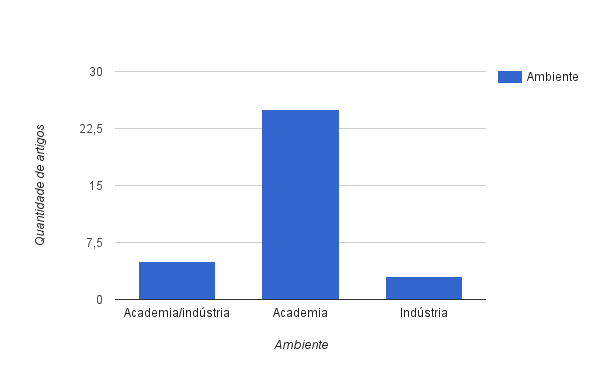
\includegraphics[scale=0.5]{tipo_de_ambiente.png}
 \caption{\label{fig:ambiente}Contagem de Artigos por Ambiente}
\end{figure}
 
 %\FloatBarrier%
 
 \begin{figure}[h!]
 \centering
 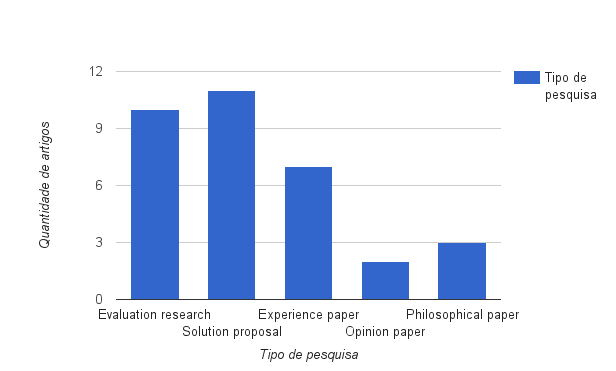
\includegraphics[scale=0.5]{tipo_de_pesquisa.png}
 \caption{\label{fig:tipo_de_pesquisa}Contagem de Artigos por Tipos de Pesquisa}
\end{figure}
 
 %\FloatBarrier%
 
 \begin{figure}[h!]
 \centering
 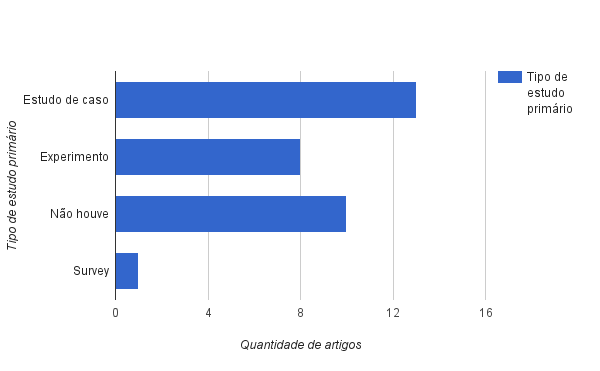
\includegraphics[scale=0.5]{tipo_de_estudo_primario.png}
 \caption{\label{fig:tipo_de_estudo_primario}Contagem de Artigos por Tipos de
 Estudos Primários}
\end{figure}
 \FloatBarrier
 
 \section{Vantagens, desvantagens e achados principais}
 
 A medida que fomos encontrando novas técnicas de negociação e catalogando suas
 vantagens, desvantagens e seus achados, era
 inevitável que fôssemos comparando as diferentes técnicas nesses quesitos.
 Algo que ficou claro, não existe uma '\textit{silver bullet}', uma técnica que
 seja ideal para qualquer tipo de projeto em qualquer organização. É possível de certa forma, dadas algumas características, escolher uma técnica que mais se enquadre à realidade dos \textit{stakeholders}. Por isso podemos seguramente
 dizer que a escolha de uma técnica é um cenário de \textit{trade-off}. O
 objetivo dessa seção é de guiar um provável usuário de técnicas de negociação
 de requisitos pelas características das mesmas auxiliando-o a descobrir qual
 a melhor opção para o seu contexto, além de responder a quarta e a quinta questões secundárias.

\subsection{Vantagens}

O \textit{WinWin}, quando aplicado usando o modelo espiral, e o \textit{WinWin
with Scrum} suportam mudanças e aceitam novos requisitos em qualquer etapa da
 negociação \cite{boehm2001developing}\cite{khan2014integration}.
O \textit{WinWin with Scrum} e o \textit{Easy WinWin} têm como vantagem um tempo
de duração menor para alcançar os objetivos
\cite{khan2014integration}\cite{briggs2002easywinwin}. Esta última e o
\textit{WinWin} abordam bem a questão de comunicação e colaboração entre os
\textit{stakeholders} \cite{grunbacher2001surfacing}\cite{boehm1998winwin}.
O \textit{Easy WinWin} chega ao ponto de tentar impedir que os
\textit{stakeholders} sejam julgados por suas opiniões
\cite{gruenbacher2000collaborative}.
O Win CBAM, o CBSP e o \textit{QA Easy WinWin} avaliam a concordância dos
\textit{stakeholders}
\cite{kazman2005requirements}\cite{grunbacher2001reconciling}\cite{grunbacher2004integrating},
sendo que estas duas últimas técnicas ainda promovem a compreensão entre
diferentes pontos de vista (técnica vs. funcional)
\cite{grunbacher2001reconciling}\cite{grunbacher2004integrating}. Enquanto a
última das mencionadas, juntamente com o \textit{WinWin}, apresentam
flexibilidade de domínio \cite{grunbacher2004integrating}\cite{boehm1997developing}, o
\textit{Quantitative WinWin} e o MPARN, diferentemente de todas as outras
técnicas, focam em adaptar o \textit{WinWin} para ter uma tomada de decisão mais
pontual e objetiva \cite{ruhe2002quantitative}\cite{in2004requirements}.


\subsection{Desvantagens}

Uma grande parte dos artigos analisados não continham estudos primários que
sustentassem achados de fato. A maioria deles, de certa forma, defendia o uso da
técnica apresentada no contexto do artigo, logo não costumavam falar diretamente
as desvantagens das técnicas. Devido a estes fatos, as desvantagens a seguir
foram resultado da nossa interpretação do material coletado de cada técnica.

No \textit{WinWin} mesmo havendo um sentimento geral de colaboração, ao final
das negociações os \textit{stakeholders} podem não se sentir completamente
satisfeitos com a especificação, porque podem, as vezes, ter cedido demais.
O \textit{WinWin} por ser bastante subjetivo \cite{ruhe2002software},pode fazer
com que sejam necessárias bem mais reuniões de negociação para analisar um set
de requisitos, do que o \textit{Easy WinWin}.
O \textit{quantitative WinWin} e MPARN são altamente dependentes de ferramentas,
visto que sendo técnicas objetivas, os \textit{stakeholders} precisam ser
guiados para não esquecer de realizar comparações. Pode-se haver perda do foco durante a tarefa
de comparação dos requisitos, caso hajam muitos a serem analisados. O MPARN ajuda para decisões locais, entretanto para decisões globais não é completamente efetivo.
\textit{Quantitative winwin}, MPARN e \textit{requeriment negotiation spiral
model} não tiveram suas vantagens comprovadas, sendo assim têm baixa
confiabilidade. \cite{ruhe2002quantitative}\cite{in2004requirements}

\subsection{Achados}

\begin{itemize}
\setlength{\itemsep}{1pt}
\setlength{\itemindent}{20pt}
\item Usuários e clientes são mais ativos em definir condições de vitória,
enquanto desenvolvedores e analistas foram mais ativos em resolver os conflitos,
tentando achar alternativas. \cite{in2001applying}
\item Existem várias formas de se aplicar o MPARN, devido a grandes quantidades
de funções para serem usadas em seus passos matemáticos. \cite{in2002multi}
\item \textit{Easy WinWin} ajuda na documentação e é interessante associá-lo a
técnica de inspeção. \cite{khan2014integration}
\item \textit{Stakeholders} tendem a aceitar condições de vitória satisfatórias
e, quando conquistadas, não se empenham com ímpeto em alcançar a solução ótima para
si. \cite{in2001applying}
\item É importante prototipar durante o desenvolvimento e negociação, para que o
usuário e cliente não mudem de ideia ao final das negociações como um todo.
\cite{boehm1998using}
\item Muitas condições de vitória podem ser alcançadas usando-se
\textit{brainstorming}.
\cite{grunbacher2001surfacing}
\item \textit{Face to face} traz sensação de segurança. \cite{egyed1997analysis}
\end{itemize} 
 
\section{Considerações Gerais da Área}

Não encontramos na literatura uma taxonomia clara e uniforme para técnicas de
negociação de requisitos. Foram encontrados, por exemplo, artigos onde
definia-se negociação como a priorização de requisitos feita apenas por um
\textit{stakeholder}. Sendo assim, não consideramos esse caso como técnica de
negociação, pois não se pode negociar consigo mesmo.

\textit{WinWin} e \textit{Spiral WinWin} são modelos de negociação de
requisitos, ou seja, são um arcabouço, cuja estrutura direciona o que deve ser alcançado. Em diversos
artigos, entretanto, eram explicitados passos que poderiam ser seguidos pelos \textit{stakeholders}. Por este motivo criamos, de certa forma, uma técnica de negociação de
requisitos chamada \textit{WinWin}.


Nos mesmos artigos onde encontramos o \textit{WinWin} e o \textit{Spiral
WinWin}, os nomes eram trocados diversas vezes, porém se referindo à um mesmo
conceito.
Como feito em \cite{boehm2006winwin}, que na introdução contextualizava o \textit{Spiral WinWin}, o qual seria a base do artigo, contudo, nas seções seguintes haviam passagens onde
falava-se do \textit{WinWin} e a imagem usada para exemplificar visualmente,
continha uma representação em espiral; outras vezes ainda no texto, tornava à aparecer
\textit{WinWin}. Dessa forma, o artigo não deixava claro se tratava de um, de
outro, ou ambos.

Eventualmente, encontrávamos artigos, cujo tema era \textit{framework}. Essa
palavra pode se referir à uma técnica ou uma ferramenta, por isso houve dificuldade de
compreensão, cabendo então interpretação.

Nossa intenção com esta revisão era encontrar uma certa variedade de técnicas de
negociação de requisitos e classificar cada uma delas, tendo como objetivo
situá-las num ambiente e contexto para permitir que \textit{stakeholders}
escolham a mais adequada, dada a conjuntura no qual eles estão inseridos. Mas o
que encontramos foi basicamente uma técnica, \textit{WinWin}, e suas diversas variações. Essas
variações abordavam diferentes focos (arquitetura, custo e etc.), bem como
diferentes formas de classificar e quantificar o valor de cada requisito.
\chapter{Conclusões}\label{cap:conclusoes}

Neste trabalho apresentamos uma revisão quasi-sistemática a respeito de técnicas
de negociação de requisitos de \textit{software}. Foram  identificados  33 
artigos  descrevendo  10  diferentes  técnicas de negociação de requisitos e
suas características. Essas características incluem sua descrição, o ambiente em
que as técnicas foram descritas, avaliadas ou aplicadas, os tipos de pesquisa
que vem sendo publicados, os tipos de estudo primário, os principais achados de
cada artigo e as vantagens e desvantagens reportadas para as técnicas. É possível observar que existem diferentes técnicas de negociação de requisitos, algumas não necessariamente são melhores que outras, mas sim diferentes. Sua efetividade dependerá do ambiente e do contexto em que os \textit{stakeholders} estão inseridos. A grande maioria dos artigos que encontramos abordam a técnica no ambiente acadêmico e pouco se fala na aplicação dessas técnicas na indústria.

No restante deste capítulo apresentamos as principais contribuições, limitações e as possibilidades de trabalhos futuros.

\section{Contribuições}
Entre as contribuições deste trabalho destacamos as seguintes:

\begin{itemize}
\setlength{\itemsep}{1pt}
\setlength{\itemindent}{20pt}
\item O planejamento de um protocolo de revisão quasi-sistemática que pode ser utilizado para obter uma visão ampla e imparcial a respeito de técnicas de negociação de requisitos de \textit{software}.
\item A execução do protocolo em entre Novembro de 2015 e Julho de 2016, identificando 33 artigos contendo 10 técnicas de negociação de requisitos.
\item Os resultados da revisão, que fornecem uma visão geral das técnicas de negociação de requisitos e de suas características, incluindo vantagens, desvantagens e os principais achados.
\end{itemize} 

Acreditamos que estas contribuições possam ser úteis tanto para pesquisadores quanto para praticantes. Pesquisadores podem fazer uso da visão geral das pesquisas nesta área para situar novas pesquisas.
Os praticantes, por sua vez, podem utilizar os resultados da revisão para auxiliar na escolha de uma técnica de negociação de requisitos. É importante destacar que a negociação de requisitos é uma atividade 
que ocorre na prática de forma inerente ao próprio processo de desenvolvimento de \textit{software}, seguindo alguma técnica ou não. Desta forma, os resultados aqui produzidos podem ser utilizados por praticantes na 
busca por oportunidades de melhoria em seus processos.

\section{Limitações}

Ao decorrer deste trabalho, tivemos algumas limitações, sendo as principais delas:
\begin{itemize}
\setlength{\itemsep}{1pt}
\setlength{\itemindent}{20pt}
\item A falta de conhecimento prévio sobre técnicas de negociação de requisitos de \textit{software}.
\item Dificuldades devido a não existência de taxonomia clara do que é uma técnica de negociação. Um exemplo desta dificuldade foi a utilização frequente da palavra \textit{framework}, que atrapalhou bastante o entendimento, visto que quando usada, não indicava se a utilização era referente a uma técnica ou a uma ferramenta.
\item Aplicamos somente o primeiro nível do \textit{Backward Snowballing}.
\item Não aplicamos O \textit{Forward Snowballing}. De fato, isso seria
inviável, visto que a quantidade de citações aos 33 artigos que analisamos é muito grande. Por exemplo, 412 artigos citam \cite{boehm1998using}, 191 artigos citam \cite{boehm1994software}, 93 artigos citam \cite{grunbacher2001surfacing} e 207 citam \cite{boehm1995software}, o que totaliza, somente neste conjunto de 4 artigos, 903 artigos a serem analisados.
\end{itemize} 

\section{Trabalhos Futuros}

Como trabalho futuro, dada a pouca quantidade de estudos referentes ao uso das
técnicas na indústria, propomos realizar estudos primários nesse ambiente. Um
exemplo seria uma \textit{survey} para verificar se as empresas usam as técnicas
encontradas, técnicas não encontradas ou se não usam nenhuma técnica. Caso o
estudo primário fosse um experimento ou estudo de caso, poderíamos ainda analisar alguns aspectos como a preferência dos \textit{stakeholders}, a viabilidade de se usar ferramentas e analisar se realmente são fundamentais ou se a técnica pode ser aplicada sem as mesmas; índice de satisfação com os resultados da negociação, se os \textit{stakeholders} perdem com frequência o foco ao aplicar a técnica, entre outros.

%%%%%%%%%%%%%%%%%%%%%%%%%%%%%%%%%%%%%%%%%%%%%%%%%%%%%%%%%%%%%%%%%%%
%                  Refer�ncias Bibliogr�ficas                     %
%%%%%%%%%%%%%%%%%%%%%%%%%%%%%%%%%%%%%%%%%%%%%%%%%%%%%%%%%%%%%%%%%%%
%Usar o bibtex
\cleardoublepage
\bibliographystyle{abnt}
\bibliography{bibliografia}%{} % arquivos fonte com a bibliografia


%%apendice
\cleardoublepage
\begin{appendices}
\chapter{Resultado da String de busca}\label{refstring}

%\definecolor{colorlabel}{HTML}{A7A6A6}

\begin{longtable}{{>{\centering\arraybackslash}m{5cm}>{\centering\arraybackslash}m{5cm}>{\centering\arraybackslash}m{5cm}}}

    %\begin{tabular}{{|>{\centering\arraybackslash}m{5cm}|>{\cente%ring\arraybackslash}m{5cm}|>{\centering\arraybackslash}m{5cm}$|}}
\hline
Titulo & Autor & Ano \\ 
\hline
From producer to creator, the implications and challenges for ireland &
Davenport, F & 2008\\
 \hline 
11th International Conference on Product Focused Software Development and Process Improvement, PROFES 2010 & Lero and  Assoc. Comput. Mach. Spec. Interest, Group and Softw, En & 2010\\
 \hline 
1st International IFIP Workshop on Autonomic Communication, WAC 2004 & Eu Commission, F E T Programme and Fraunhofer, Fokus and Ifip, W & 2005\\
 \hline 
2010 4th International Workshop on Software Product Management, IWSPM 2010 &   & 2010\\
 \hline 
2012 International Conference on Software and System Process, ICSSP 2012 - Proceedings & International Software Process, Associatio & 2012\\
 \hline 
2013 International Conference on Mechanical and Electronics Engineering, ICMEE 2013 & Tianjin University of, Technology and Kagawa, University and  Hefei University of, Technolog & 2013\\
 \hline 
25th annual international computer software and applications conferenc & Society, Ieee Compute & 2001\\
 \hline 
3rd International Conference on Electronic Government, EGOV 2004 &   & 2004\\
 \hline 
A bargaining-specific architecture for supporting automated service agreement
negotiation systems & Resinas, M and Fern \' andez, P and Corchuelo, R & 2012\\
 \hline 
A Cloud Service Broker for SLA-based SaaS provisioning & Badidi, E & 2013\\
 \hline 
A coalition formation based model for web service composition & Maya, S B and  Natl. Agency Dev. Univ, Res and  Head Off. Sci. Res. Technol, Dev and  French Embassy in, Algiers and  the French Institute of, Algeria and Program, Cmep Tassili and  Auth. Regul. Post Off, Telecommu & 2012\\
 \hline 
A cognitive psychology approach for balancing elicitation goals & Carod, N M and Cechich, A and Society, Ieee Computer and Ieee, Icci and University of, Calgary and  California State, Universit & 2007\\
 \hline 
A collaborative approach to requirements elicitation & Laporti, V and Borges, M R S and Braganholo, V P and  Swinburne University of, Technology and Section, Ieee Victoria and  International Working Group on Cscw in Design, Cscw & 2007\\
 \hline 
A compromise-negotiation framework based on game theory for eliminating
requirements inconsistency & Feng, T and Zhang, Y R and Jin, Y and Zhang, J &
2015\\
 \hline 
A conceptual model for negotiating in service-oriented environments & Lin, J &
2008\\
 \hline 
A conceptual model of an interorganizational intelligent meeting-scheduler (IIMS) & Glezer, & 2003\\
 \hline 
A context and service-oriented architecture with adaptive quality of service support & Hafez, D and Aly, S G and Sameh, & 2011\\
 \hline 
A distributed agent system for port planning and scheduling & Yin, X F and Khoo, L P and Chen, C & 2011\\
 \hline 
A distributed multi-agent meeting scheduler & Shakshuki, E and Koo, H H and Benoit, D and Silver, & 2008\\
 \hline 
A flexible, agent-based ICT architecture for virtual enterprises & Aerts, A T M and Szirbik, N B and Goossenaerts, J B & 2002\\
 \hline 
A framework for Distributed decision support Multi-Agent Intelligent System & El-Ghamrawy, S M and El-Desouky, A & 2008\\
 \hline 
A framework for experimenting with QoS for multimedia services & Chen, D and Colwell, R and Gelman, H and Chrysanthis, P K and Moss \' e, & 1996\\
 \hline 
A framework for integrated negotiation support system & Lei, Y and Feng, Y Q and  Ieee Systems, Man and  Cybernetics Techn, Committee and  Shanghai Jiao Tong, University and  Hong Kong Polytechnic, University and  Int. University of, Germany and Hebei, Universit & 2004\\
 \hline 
A framework for multi-valued reasoning over inconsistent viewpoints & Easterbrook, S and Chechik, M and Ieee and Acm, Sigsof & 2001\\
 \hline 
A framework for QoS-aware software components & Menasc \' e, D A and Ruan, H and Gomaa, & 2004\\
 \hline 
A framework for supporting dynamic systems co-evolution & Morrison, R and Balasubramaniam, D and Kirby, G and Mickan, K and Warboys, B and Greenwood, R M and Robertson, I and Snowdon, & 2007\\
 \hline 
A framework for the evaluation of an electronic marketplace design with evolutionary negotiation support & Cho, & 2001\\
 \hline 
A fuzzy system approach to multilateral automated negotiation in B2C e-commerce & Shojaiemehr, B and Rafsanjani, M & 2013\\
 \hline 
A fuzzy system approach to multilateral automated negotiation in B2C e-commerce & Shojaiemehr, B and Rafsanjani, M & 2014\\
 \hline 
A hybrid approach to upstream requirements: IBIS and cognitive mapping & Rooksby, J and Sommerville, I and Pidd, & 2006\\
 \hline 
A Measurement-Driven Process Model For Managing Inconsistent Software Requirements & Mu, K and Jin, Z and Zowghi, D and  Institute of Software, Chinese Academy of Sciences Isca & 2008\\
 \hline 
A method product quality control between enterprises and its implementation & Tian, J and Lv, J and  Huazhong Normal, University and  Huazhong University of, Science and Technology and  Research Association of Modern, Education and Computer, Science and Columbia, University and Wuhan, Universit & 2010\\
 \hline 
A methodology of collaborative requirements validation in a cooperative environment & Sourour, M D and Zarour, N and Solutions, I T and University of, Sciences and  Technologies Houari, Boumediene and Lria and Lsi and Mpti & 2011\\
 \hline 
A model for requirements negotiation in software ecosystems & Valen \c ca, G and Alves, & 2013\\
 \hline 
A multi-agent infrastructure for mobile workforce management in a service oriented enterprise & Chiu, D K W and Cheung, S C and Leung, H F and Society, Ieee Compute & 2005\\
 \hline 
A multi-agent, multi-object and multi-attribute intelligent negotiation model & Fei, Y and Chen, & 2007\\
 \hline 
A negotiation framework for managing the requirements changes & Zhang, Y and Jin, Y and Bai, J and Zhang, & 2013\\
 \hline 
A negotiation-based networking methodology to enable cooperation across heterogeneous co-located networks & De Poorter, E and Becue, P and Rovcanin, M and Moerman, I and Demeester, & 2012\\
 \hline 
A Pattern-based approach for analysing requirements in socio-technical systems engineering & Hoffmann, A and Ieee and Society, Ieee Computer and  International Requirements Engineering, Board and  Center of Excellence for Software, Traceability and  University of Minnesota Software Engineering, Cente & 2012\\
 \hline 
A petri net model of distributed control in a holonic manufacturing execution system & Demongodin, I and Hennet, J & 2008\\
 \hline 
A priority-based negotiations approach for handling inconsistencies in multi-perspective software requirements & Mu, K and Jin, Z and Zowghi, & 2008\\
 \hline 
A QoS negotiation protocol for grid workflow & Yong, W and Li, W and Chunming, & 2006\\
 \hline 
A quality of service framework for dependability in large-scale distributed systems & Bull, P and Guan, L and Phill, I and Grigg, A and Society, Ieee Compute & 2011\\
 \hline 
A requirements negotiation model based on multi-criteria analysis & In, H and Olson, D and Rodgers, T and Iee & 2001\\
 \hline 
A review of negotiation techniques in component based software engineering & Hutchinson, J and Kotonya, & 2006\\
 \hline 
A risk management investigation of SME adoption of agile method information system development & Clutterbuck, & 2009\\
 \hline 
A risk-driven method for eXtreme programming release planning & Mingshu, L and Meng, H and Fengdi, S and Juan, L and  Acm Special Interest Group on Software Engineering, Sigsof & 2006\\
 \hline 
A security gateway application for End-to-End M2M communications & Chen, H C and You, I and Weng, C E and Cheng, C H and Huang, Y & 2015\\
 \hline 
A service model for component-based development & Hutchinson, J and Kotonya, G and Sommerville, I and Hall, & 2004\\
 \hline 
A similarity model for virtual networks negotiation & Gomes, R L and Bittencourt, L F and Madeira, E R M and Computing, A C M Special Interest Group on Applie & 2014\\
 \hline 
A SNAP-based community resource broker using a three-phase commit protocol: A performance study & Haji, M H and Gourlay, I and Djemame, K and Dew, P & 2005\\
 \hline 
A study of developer attitude to component reuse in three IT companies & Li, J and Conradi, R and Mohagheghi, P and S, O A and Wang,  and Naalsund, E and Walseth, O & 2004\\
 \hline 
A study of emotions in requirements engineering & Colomo-Palacios, R and Hern \' andez-L \' opez, A and Garc \' ia-Crespo,  \' A and Soto-Acosta, & 2010\\
 \hline 
A systematic approach for evaluation and selection of ERP systems & Alpers, S and Becker, C and Eryilmaz, E and Schuster, & 2014\\
 \hline 
A systematic classification and analysis of NFRs & Loucopoulos, P and Sun, J and Zhao, L and Heidari, F and Ibm and Alliances, S A P University and Microsoft and DePaul, University and  Georgia State University, J Mack Robinson College of Business and Et al & 2013\\
 \hline 
A uniform negotiation and delivery mechanism for SIP-based conferencing system & Zhang, W and Lei, W and Tian, K and Zhang, & 2009\\
 \hline 
A web-enabled engineering object modeling environment to support interoperability and intelligent services in collaborative design & Yang, Q Z and Lu, W F and Division, Asme Design Engineering and Computers, Asme and  Information in Engineering, Divisio & 2005\\
 \hline 
Absolute scales to express stakeholder value for improving support for prioritization & Brodie, L and Woodman, & 2010\\
 \hline 
Access control policy negotiation for remote hot-deployed grid services & Xue, W and Huai, J and Liu, & 2005\\
 \hline 
Accommodating disagreement: A study of effective design collaboration & McDonnell, & 2012\\
 \hline 
Achieving best value in private finance initiative project procurement & Akintoye, A and Hardcastle, C and Beck, M and Chinyio, E and Asenova, & 2003\\
 \hline 
Acquiring domain knowledge for negotiating agents: A case of study & Castro-Schez, J J and Jennings, N R and Luo, X and Shadbolt, N & 2004\\
 \hline 
Adaptive agent negotiation for software process modeling & Li, N and Li, M S and Wang, Q and Zhao, C and Du, S & 2009\\
 \hline 
Adaptive business intelligence for an open negotiation environment & Aciar, S and Avesani, P and  De La Rosa, J L and Hormazabal, N and Serra, & 2009\\
 \hline 
Adaptive out-of-band routing protocol auto-negotiation for mobile ad hoc networks & Battenfeld, O and Reinhardt, P and Freisleben, & 2007\\
 \hline 
Adaptive personal service environment & Sihvonen, & 2007\\
 \hline 
Addressing the conflicting dimension of groupware: A case study in software requirements validation & Antunes, P and Ramires, J and Resp \' icio, & 2006\\
 \hline 
Advanced decision support: Improving control room effectiveness & Garnsworthy, J and Zanconato, R and Soltysiak, S and  Wessex Institute of Technology, Southampton U & 2004\\
 \hline 
Agent and Multi-Agent Systems: Technologies and Applications - First KES International Symposium, KES-AMSTA 2007, Proceedings &   & 2007\\
 \hline 
Agent based cloud provisioning and management: Design and prototypal implementation & Venticinque, S and Aversa, R and  Di Martino, B and Petcu, D and  Inst. Syst. Technol. Inf, Control Commu & 2011\\
 \hline 
Agent modeling of user preferences based on fuzzy classified ANNs In automated negotiation & Gu, T J and Tang, B Y and Ma, X J and Li, & 2011\\
 \hline 
Agent negotiation for different needs in smart parking allocation & Di Napoli, C and  Di Nocera, D and Rossi, S and Aepia and Afia and Ibm and Spain, Ieee Smc and University of, Salamanca and Et al & 2014\\
 \hline 
Agent support for context-aware services and personal mobility & El-Khatib, K and Bochmann, G & 2003\\
 \hline 
Agent-based cloud computing & Sim, K & 2012\\
 \hline 
Agent-based multiservice negotiation for eCommerce & Merlat, & 1999\\
 \hline 
Agent-based negotiation and decision making for dynamic supply chain formation & Wang, M and Wang, H and Vogel, D and Kumar, K and Chiu, D K & 2009\\
 \hline 
Agent-based negotiation framework for web service's SLA & Al-Aaidroos, M and Jailani, N and Mukhtar, & 2011\\
 \hline 
Agent-based service-oriented computing and applications & Shen, W and Ghenniwa, H and Li, & 2007\\
 \hline 
Agent-mediated off-exchange trading & Weinhardt, Christof and Gomber, Peter and Iee & 1999\\
 \hline 
Agent-oriented manufacturing scheduling services for enterprise cooperation & Hao, Q and Shen, W and Wang, & 2005\\
 \hline 
Agile commitments: Dealing with business expectations risks in agile development & Concha, M and Visconti, M and Astudillo, & 2007\\
 \hline 
Agile commitments: Enhancing business risk management in agile development projects & Concha, M and Visconti, M and Astudillo, & 2007\\
 \hline 
Agile principles as a leadership value system in the software development: Are we ready to be unleashed? & Patil, S B and Rao, S and Patil, P S and  Thakur College Of, Engineering and Technology and Intelligence, A C M Special Interest Group on Artificia & 2011\\
 \hline 
Agile processes and modeling & Larman, & 2003\\
 \hline 
AMD based service agent collaboration and specification & Zheng, L and Ieee and Society, Ieee Compute & 2014\\
 \hline 
An agent-based application to enable deregulated energy markets & Capodieci, N and Cabri, G and Pagani, G A and Aiello, M and Ieee and Society, Ieee Compute & 2012\\
 \hline 
An agent-based compositional framework & Anane, R and Li, Y and Tsai, C F and Chao, K M and Younas, M and  National Institute of, Inf and  Commun. Technol, Nict Japan and  Shanghai Jiao Tong University, China and  Victoria University, Australia and  National Natural Science Foundation of, China and  Arc Res. Network on Enterprise Inf. Infrastructure, Australi & 2005\\
 \hline 
An agent-based negotiation support system with fuzzy multi-objective decision-making method & Meng, Y and Meng, B and  Ieee Systems, Man and Cybernetics, Society and  Chongqing University, Ceba and  Tsinghua University, Res Center for Contemporary Manag & 2005\\
 \hline 
An agent-based perspective to handover management in 4G networks & Zafeiris, V E and Giakoumakis, E & 2008\\
 \hline 
An agent-based platform for contract negotiation in power market & Minpeng, X and Jiahai, Y and Changhong, & 2005\\
 \hline 
An agent-based system for multi-project planning and scheduling & Li, J and Liu, W and Ieee and Robotics and Automation, Society and  Harbin Engineering, University and  Robotics Society of Japan, R S J and  University of Eelectronic, Science and Technology of, Chin & 2005\\
 \hline 
An agent-oriented approach to requirements engineering & Gaur, V and Soni, A and Bedi, & 2010\\
 \hline 
An approach to estimate the savings from negotiation based on cost-benefit analysis model & Ahmad, S and Muda, A K and Muda, N A and Othman, & 2011\\
 \hline 
An approach to modeling context-adaptable services & Kim, Y and Doh, K & 2007\\
 \hline 
An architectural approach for dynamic web service composition & Petrova-Antonova, D and Ilieva, & 2012\\
 \hline 
An architecture-centric development environment for black-box component-based systems & Kotonya, & 2008\\
 \hline 
An economic model for resource management in a Grid-based content distribution network & Di Stefano, A and Santoro, & 2008\\
 \hline 
An efficient and minimum sensitivity cost negotiation strategy in automated trust Negotiation & Yan, H and Miaoliang, Z and Chunying, & 2008\\
 \hline 
An empirical assessment of the use of different communication modes for requirement elicitation and negotiation using students as a subject & Rodina, A and Amjed, T and Zarinah, M K and /Ind, Ieee Malaysia Power Electron. and  Electron. / Ind. Appl. Jt, Chapte & 2012\\
 \hline 
An empirical investigation on text-based communication in distributed requirements workshops & Calefato, F and Damian, D and Lanubile, F and Engineering, Ieee Computer Society Technical Committee on Softwar & 2007\\
 \hline 
An empirical study of developers views on software reuse in statoil ASA & Slyngstad, O P N and Gupta, A and Conradi, R and Mohagheghi, P and R Onneberg, H and Landre, E and Engineering, A C M Special Interest Group on Softwar & 2006\\
 \hline 
An empirical study of facilitation of computer-mediated distributed requirements negotiations & Damian, D E H and Eberlein, A and Woodward, B and Shaw, M L G and Gaines, B R and Iee & 2001\\
 \hline 
An empirical study of requirements engineering in distributed software projects: Is distance negotiation more effective? & Damian, D and  National Natural Science Foundation of, China and Public, Administration and  Civil Service Bureau of Macau, S A R and  Companhia de Telecomunicacoes de Macau, S A R L and Macau, S A R Government Tourist Offic & 2001\\
 \hline 
An empirical study of the complex relationships between requirements engineering processes and other processes that lead to payoffs in productivity, quality, and risk management & Damian, D and Chisan, & 2006\\
 \hline 
An empirical study of the impact of asynchronous discussions on remote synchronous requirements meetings & Damian, D and Lanubile, F and Mallardo, & 2006\\
 \hline 
An enhanced wiki for requirements engineering & Ferreira, D D A and  Da Silva, A & 2009\\
 \hline 
An evaluation of formalisms for negotiations in E-commerce & Benyoucef, M and Keller, R K and Apiiq and Cirano and Gi and Laval, University and Sg & 2000\\
 \hline 
An evolutionary computation approach to electricity trade negotiation & Al-Agtash, S Y and Al-Fahoum, A & 2005\\
 \hline 
An experimental design to exercise negotiation in requirements engineering & Ahmad, S and Muda, N A and Springe & 2011\\
 \hline 
An integration system of video-based interaction and online negotiation in real-time processing of E-commerce order & Hu, X and Cheng, Q and Huang, & 2008\\
 \hline 
An OCCI compliant interface for IAAS provisioning and monitoring & Venticinque, S and Amato, A and  Di Martino, B and  Inst. Syst. Technol. Inf, Control Commu & 2012\\
 \hline 
An ontology framework for EC automated negotiation protocol & Ji, S and Liang, Y and Tian, Q and Yang, & 2007\\
 \hline 
An SLA negotiation strategy for scheduling in grid & Arshad Sharafeh, S and Moghadam, N and Sanei, & 2012\\
 \hline 
Analysis of the dynamic performance of the new-type 160 km  \textperiodcentered h-1 special container flat car & Meng, H and Zhai, W and Wang, K and An, & 2009\\
 \hline 
Analytic evaluation of groupware design & Antunes, P and Borges, M R S and Pino, J A and Carri \c co, & 2006\\
 \hline 
Analyzing differences in risk perceptions between developers and acquirers in OTS-based custom software projects using stakeholder analysis & Kusumo, D S and Staples, M and Zhu, L and Jeffery, R and Engineering, A C M Special Interest Group on Software and Society, Ieee Compute & 2012\\
 \hline 
Analyzing groupware design by means of usability results & Antunes, P and Borges, M R S and Pino, J A and Carri \c co, L and  Coventry University, U K and Institute of, Electrical and  Electronics Engineers, Ieee and  Institution of Electrical Engineers, I E E and  British Computer Society, B C & 2005\\
 \hline 
Analyzing shared workspaces design with human-performance models & Antunes, P and Ferreira, A and Pino, J A and  Junta de Castilla y Leon, Spain and  Ministerio de Educacion y Ciencia, Spain and  Universidad de Valladolid, Spai & 2006\\
 \hline 
ANIS: A negotiated integration of services in distributed environments & Ibrahim, N and  Le Mouel, & 2006\\
 \hline 
Applied ontology for Requirments Engineering: An approach to semantic integration of requirements model with system model & Mir, M S and Agarwal, N and Iqbal, K and  Int. Assoc. Sci. Technol, De & 2011\\
 \hline 
Applying self-organizing agents to university class scheduling & Nunohiro, E and Mackin, K & 2003\\
 \hline 
ASREF: An adaptive service requirements elicitation framework based on goal-oriented modelling & Qiao, W and Liu, L and Xiang, & 2008\\
 \hline 
Assessing communication media richness in requirements negotiation & Erra, U and Scanniello, & 2010\\
 \hline 
Assessing requirements compliance scenarios in system platform subcontracting & Regnell, B and Olsson, H O and Mossberg, & 2006\\
 \hline 
Assisting Decision Making in Requirements Reconciliation & Richards, D and Boettger, K and Faperj and Sbc and Ufri and Ieee and Coppetec, Fundaca & 2002\\
 \hline 
Asynchronous negotiation and collaboration of software requirements for an emergency response information system: An empirical investigation & Campbell, C L and  Van De Walle, B A and Deek, F P and Lab, Decis and Societies, Euro The Association of European Operational Research and Groupsupport.com and Intergraph, Corporation and  Prolog Development Center, A S and Respond, B & 2005\\
 \hline 
Asynchronous requirements engineering: Enhancing distributed software development & Campbell, C L and  Van De Walle, B and  New Jersey Institute of, Technology and Section, Ieee North Jersey and Chapter, Ieee Comsoc North Jerse & 2003\\
 \hline 
Automated negotiation for service contracts & Lock, & 2006\\
 \hline 
Automated negotiations in web service procurement & Patankar, V and Hewett, R and Iari & 2008\\
 \hline 
Automated SLA negotiation framework for cloud computing & Wu, L and Garg, S K and Buyya, R and Chen, C and Versteeg, & 2013\\
 \hline 
Automatic services instantiation based on a process specification & Borges, H P and  De Souza, J N and Schulze, B and Mury, A & 2014\\
 \hline 
Automating cloud services life cycle through semantic technologies & Joshi, K P and Yesha, Y and Finin, & 2014\\
 \hline 
Automating human based negotiation processes for autonomic logistics & Karsai, G and Bloor, G and Doyle, J and Iee & 2000\\
 \hline 
Balancing load of shaper in WikiWinWin requirements negotiation environment: An empirical evaluation & Wan, P and Huang, S and Li, J and Yang, D and Yang, Y and Lero and  Assoc. Comput. Mach. Spec. Interest, Group and Softw, En & 2010\\
 \hline 
Bargain shopping searching for inexpensive programmable-logic assistance & Dipert, & 2003\\
 \hline 
Best practices guidelines for agile requirements engineering practices & Patel, C and Ramachandran, & 2009\\
 \hline 
Challenges in Managing ISO 26262 Software Development Projects & Sturmer, I and Doerr, H and End, T and Avl and Continental and Fev and  Fiat Chrysler, Automobiles and Engineering, I A V Automotive and Et al & 2015\\
 \hline 
Channel-based Unidirectional Stream Protocol (CUSP) & Terpstra, W W and Leng, C and Lehn, M and Buchmann, & 2010\\
 \hline 
Clean water atlanta enterprise GIS & Brown, C and Toomer, & 2007\\
 \hline 
Cloud computing reduces uncertainties in quality-of-service matching! & Becker, M and Platenius, M C and Becker, & 2015\\
 \hline 
Coalesced QoS: A pragmatic approach to a unified model for KLOS & Chawla, A and Yerraballi, R and Vasudevan, & 2006\\
 \hline 
Coalition formation for resource coallocation using BDI assignment agents & Seow, K T and Sim, K M and Kwek, S Y & 2007\\
 \hline 
Cognitive influences in prioritizing software requirements & Carod, N M and Cechich, A and  Inst. Syst. Technol. Inf, Control Commun and University of, Piraeus and  University of Piraeus - Research, Cente & 2010\\
 \hline 
Cognitive profiles in understanding and prioritizing requirements: A case study & Carod, N M and Cechich, A and Iari & 2010\\
 \hline 
Cognitive-driven requirements prioritization: A case study & Carod, N M and Cechich, A and Society, Ieee Computer and  Natural Science Foundation of, China and Microsoft, Research and The, Ieee Icci Steering Committee and Tsinghua, Universit & 2010\\
 \hline 
Collaborative negotiation platform using a dynamic multi-criteria decision model & Arrais-Castro, A and Varela, M L R and Putnik, G D and Ribeiro, R and Dargam, F C & 2015\\
 \hline 
Collaborative planning processes & Fischer, J G and Gneiting, & 2008\\
 \hline 
Collaborative resolution of requirements mismatches when adopting open source components & Anh, N D and Cruzes, D S and Conradi, R and Host, M and Franch, X and Ayala, C and Technology, Paluno The Ruhr Institute for Software and  adesso - Business People, Technology and Sophist and  International Requirements Engineering, Board and Logic & 2012\\
 \hline 
Collaborative robotic team design and integration & Spofford, John and Anhalt, David and Herron, Jennifer and Lapin, Brett and Spi & 2000\\
 \hline 
Collaborative tools for mobile requirements acquisition & Seyff, N and Society, Ieee Computer and  Austrian Computer, Society and Acm, Sigsoft and Acm, Sigar & 2004\\
 \hline 
Combinatorial business transactions: A way for increasing the flexibility and
reliability of electronic marketplaces & Puustjärvi, & 2008\\
 \hline 
Communications management in scrum projects & Holzmann, V and Panizel, & 2013\\
 \hline 
\rowcolor[RGB]{167, 166, 166}
Comparing software system requirements negotiation
patterns & Egyed, A and Boehm, &
1999\\
 \hline 
Comparing the effect of use case format on end user understanding of system requirements & Mustafa, B & 2010\\
 \hline 
Comparison of requirements hand-off, analysis, and negotiation: Case study & Fricker, S and Glinz, M and Ieee and  University of Technology, Sydney and Society, Ieee Computer and Hctd and DePaul, Universit & 2010\\
 \hline 
Competition and collaboration in requirements engineering: A case study of an emerging software ecosystem & Valen \c ca, G and Alves, C and Heimann, V and Jansen, S and Brinkkemper, S and  Blekinge Tekniska, Hogskola and Cisco and Ieee and  Iowa State University - College of Liberal, Arts and Sciences and  Sweden at its Best, Visitblekinge Se and Et al & 2014\\
 \hline 
Composing RESTful services with jOpera & Pautasso, & 2009\\
 \hline 
Composition of aspectual requirements: A multi-criteria process for conflict resolution & Amroune, M and Zarour, N and Charrel, P J and Inglebert, J & 2014\\
 \hline 
Computer-mediated communication to support distributed requirements elicitations and negotiations tasks & Calefato, F and Damian, D and Lanubile, & 2012\\
 \hline 
Computing pareto optimal agreements in multi-issue negotiation for service composition & Di Napoli, C and  Di Nocera, D and Rossi, S and Acm, Sigai and Argela and Artificial, Intelligence and  International Foundation for Autonomous, Agents and Multiagent, Systems and Nsf and Et al & 2015\\
 \hline 
CONCENSUS: Multi-party negotiation support for conflict resolution in concurrent engineering design & Cooper, S and Taleb-Bendiab, & 1998\\
 \hline 
Concurrent negotiation and coordination for grid resource coallocation & Sim, K M and Shi, & 2010\\
 \hline 
Constraint-based support for negotiation in collaborative design & Lottaz, C and Smith, I F C and Robert-Nicoud, Y and Faltings, B & 2000\\
 \hline 
Consumer-centric service aggregation: Method and its supporting framework & Liu, X Z and Huang, G and Mei, & 2007\\
 \hline 
Content analysis of online interrater Reliability using the Transcript Reliability Cleaning Percentage (TRCP): A software engineering case study & Oriogun, P K and Accenture and  Grupo Portucel, Soporcel and Ibm and Xerox and Xetcopi and Et al & 2003\\
 \hline 
Contracts for security adaptation & Mart \' in, J A and Pimentel, & 2011\\
 \hline 
CORAMOD: A checklist-oriented model-based requirements analysis approach & Brace, W and Ekman, & 2014\\
 \hline 
Customer collaboration: How to replace our old semi-hostile habits with friendship and rich communication full day workshop & Jepsen, & 2004\\
 \hline 
Cyber-physical system design contracts & Derler, P and Lee, E A and Torngren, M and Tripakis, & 2013\\
 \hline 
Cyber-physical system design contracts & Derler, P and Lee, E A and Törngren, M
and Tripakis, S and Systems, A C M Special Interest Group on Embedded and Systems, T C on Real-Tim & 2013\\
 \hline 
DARYN—A Distributed Decision-Making Algorithm for Railway Networks: Modeling and Simulation & Iyer, R V and Ghosh, & 1995\\
 \hline 
Decision analysis for an Afghanistan Sustainable Infrastructure Plan (ASIP) with volatile emergent conditions & Javed, O and Melnick, M J and Reaves, D S and Todd, J W and Karvetski, C W and Lambert, J H and  Inst. Electr. Electron, Eng and Syst, Man Cybern So & 2009\\
 \hline 
Demonstration of the multi-agent simulator of competitive electricity markets & Pinto, T and Pra \c ca, I and Santos, G and Vale, & 2013\\
 \hline 
Design and evaluation of P2P overlays for energy negotiation in smart micro-grid & Amato, A and  Di Martino, B and Scialdone, M and Venticinque, & 2015\\
 \hline 
Design and implementation of a Centralized Sensor Protocol for Information via Negotiation & Pham, T H and Li, X J and Chong, P H J and Leong, Y W and  Int. Assoc. Comput. Sci. Inf, Techno & 2010\\
 \hline 
Design for information systems which can adapt to changing organizational requirements & Sillince, J A & 1994\\
 \hline 
Design on the framework of management information system for enterprises based on e-commerce & Li, Y and Yu, J and  Int. Assoc. Comput. Sci. Inf, Techno & 2010\\
 \hline 
Designing service negotiation entities for the electronic market-place & D'Antonio, S and Fadini, B and Romano, S P and Ventre, & 2002\\
 \hline 
Development of configurable e-marketplaces based on a flexible management of e-negotiation protocols & Fabra, J and  \' Alvarez, P and Ezpeleta, & 2008\\
 \hline 
Development with off-the-shelf components: 10 facts & Li, J and Conradi, R and Bunse, C and Torchiano, M and Slyngstad, O P N and Morisio, & 2009\\
 \hline 
Discovering early aspects & Baniassad, E and Clements, P C and Ara \' ujo, J and Moreira, A and Rashid, A and Tekinerdogan, & 2006\\
 \hline 
Distributed automatic configuration of complex IPsec-infrastructures & Rossberg, M and Schaefer, G and Strufe, & 2010\\
 \hline 
Domain engineering to ensure flexibility on interaction laws of multi-agent systems & Carvalho, G R and Paes, R B and Lucena, C J P and Choren, & 2007\\
 \hline 
DPP: An agent-based approach for distributed process planning & Wang, L and Shen, & 2003\\
 \hline 
DRE-specific wikis for distributed requirements engineering: A review & Peng, R and Lai, H and Chapter, A C M Hong Kong and Chapter, Ieee Hong Kong Section Computer Societ & 2012\\
 \hline 
Dynamic architectural connectors in cooperative software systems & Jiao, W and Mei, H and  Ieee Computer Society, Tccx and hina  Shanghai Jiao Tong University & 2005\\
 \hline 
DYSCO: A platform for dynamic QoS-aware web service composition & Petrova-Antonova, D and Ilieva, & 2012\\
 \hline 
E-contracting with price configuration for Web services and QoS & Marchione, F G and Fantinato, M and  De Toledo, M B F and  De Souza Gimenes, I & 2010\\
 \hline 
E-negotiation system based on intelligent agents in B2C E-commerce & Ahmadi, K D and Charkari, N M and Enami, & 2011\\
 \hline 
E-requirements negotiation: Electronic negotiations in the distributed software development & Herzwurm, G and Schoop, M and Reiser, A and Krams, B and  Volkswagen Financial, Services and Sap and Karriere, T Deutsche Telekom: and Ibm and Offentlich & 2012\\
 \hline 
EasyWinWin: A groupware-supported methodology for requirements negotiation &
Boehm, B and Grünbacher, P and Briggs, R O and Ieee and Acm, Sigsof & 2001\\
 \hline 
EasyWinWin: A groupware-supported methodology for requirements negotiation &
Grünbacher, P and Boehm, B and Wien, T U and Cepis and Sig, Sof & 2001\\
 \hline 
Effects of communication media on group performance in requirements engineering & Damian, Daniela E Herlea and Eberlein, Armin and Shaw, Mildred L G and Gaines, Brian R and Society, Ieee Compute & 2000\\
 \hline 
Efficient management of multi-linked negotiation based on a formalized model & Zhang, X and Lesser, V and Abdallah, & 2005\\
 \hline 
Electronic brokering for assisted contracting of software applets & Robinson, William N and Iee & 1997\\
 \hline 
Electronic commerce negotiation in a supply chain via constraint evaluation & Wilhelm, R and Chu, B and Sun, & 2005\\
 \hline 
Electronic contract negotiation as an application niche for mobile agents & Griffel, Frank and  Tuan Tu, M and Muenke, Malte and Merz, Michael and Lamersdorf, Winfried and da Silva, Miguel Mira and Iee & 1997\\
 \hline 
Empirical study of Sommerville and Sawyer's requirements engineering practices & Cox, K and Niazi, M and Verner, & 2009\\
 \hline 
Enabling technology for distributed multimedia applications & Wong, J W and
Lyons, K A and Evans, D and Velthuys, R J and Bochmann, G V and Dubois, E and
Georganas, N D and Neufeld, G and Özsu, M T and Brinskelle, J and Hafid, A and Hutchinson, N and Iglinski, P and Kerherv \' e, B and Lamont, L and Makaroff, D and Szafron, & 1997\\
 \hline 
End-to-end architecture for cognitive reconfigurable wireless networks & Boufidis, Z and Alonistioti, N and Holland, O and Feuillette, R and Pan, J and Moessner, & 2007\\
 \hline 
End-to-end QoS management architecture & Shankar, Mallikarjun and  De Miguel, Miguel and Liu, Jane W S and Society, Ieee Compute & 1999\\
 \hline 
Engineering emergent behaviour: A vision & Serugendo, G & 2003\\
 \hline 
Engineering of quality requirements as perceived by near-shore development centers' architects in eastern Europe: The hole in the whole & Daneva, M and Marczak, S and Herrmann, A and Software, Ieee and Microsoft, Research and Politecnico di, Torino and  Telecom Italia, J O L and  Telecom Italia, La & 2014\\
 \hline 
Engineering the software requirements of nonprofits - A service-learning approach & Venkatagiri, S and  Acm Special Interest Group on Software Engineering, Sigsof & 2006\\
 \hline 
Enhancing GSS-based requirements negotiation with distributed and mobile tools &
Seyff, N and Hoyer, C and Kroiher, E and Grünbacher, P and Engineering, Ieee Computer Society Technical Committee on Data and  The Concurrent Engineering Research Center, Cerc and  West Virginia University, U S & 2005\\
 \hline 
Enhancing interoperability: Ontology-mapping in an electronic institution & Lopes Cardoso, H and Teixeira, D D and Oliveira, & 2009\\
 \hline 
Enterprise knowledge modelling: Facilitating flexible dynamically changing systems & Loucopoulos, & 2014\\
 \hline 
Enterprise-wide solutions architecting using UML & Feldman, D and Micallef, J and Mulcare, D and Systems, Ieee Computer Society Technical Committee on Engineering of Computer-Base & 2003\\
 \hline 
Evaluating software maintenance effort: The COME matrix & Chua, B B and Verner, & 2011\\
 \hline 
Evaluating the value-added benefits of using requirements reuse metrics in ERP projects & Daneva, M and Acm/Sigsof & 2001\\
 \hline 
Evaluation of a simulation platform for interaction training: A multi-phased methodology & Monasor, M J and Vizca \' ino, A and Piattini, M and Noll, J and Beecham, S and Research, Asee Educational and Methods, Division and Society, Ieee Computer and Society, Ieee Education and  Madrid Technical, University and  Spanish University of Distance, Education and Et al & 2015\\
 \hline 
Evolutionary negotiation strategies in emerging electricity markets & Al-Agtash, & 2004\\
 \hline 
Expanding the concept of requirements traceability: The role of electronic records management in gathering evidence of crucial communications and negotiations & Chen, H and Nunes, M B and Zhou, L and Peng, G & 2011\\
 \hline 
ExPlanTech: Applying multi-agent systems in production planning & Pechoucek, M and Riha, A and Vokrinek, J and Marik, V and Prazma, & 2002\\
 \hline 
Feature interaction analysis in the advanced intelligent network: a telephone company perspective & McConnell, Von K and Nilson, Margaret E and Silverstein, Elenita E and Iee & 1993\\
 \hline 
Finding success in rapid collaborative requirements negotiation using wiki and shaper & Shidler College of, Business and University of, Hawai' & 2010\\
 \hline 
Flexible processes for evolvable products & Ghezzi, & 2005\\
 \hline 
Flexible-sense optical transmission & Rozental, V N and Bruno, G and Soso, A and Camera, M and Mello, D A & 2013\\
 \hline 
Formalizing an engineering approach to cooperating knowledge-based systems & Deen, S M and Johnson, C & 2003\\
 \hline 
Framework for agent-based buying decision process & Razali, S and Osman, & 2006\\
 \hline 
\rowcolor[RGB]{167, 166, 166}
From requirements negotiation to software architecture
decisions & Kazman, R and In, H P and Chen, H &
2005\\
 \hline 
Fuzzy complexity assessment model for resource negotiation and allocation in agent-based software testing framework & Ponnurangam, D and Uma, G & 2005\\
 \hline 
Goal oriented requirements engineering-A review & Aljahdali, S and Bano, J and Hundewale, N and  Int. Soc. Comput. Their, App & 2011\\
 \hline 
Goal-oriented requirements engine ring: A roundtrip from research to practice & Van Lamsweerde, A and  Ieee Computer Society, Technical Council on Software Eng Tcse and  Information Processing Society of Japan, Ips & 2004\\
 \hline 
Green manufacturing of ammunition through knowledge management with distributed access & Dogru, Ali H and Tanik, Murat M and Kurfess, Franz and Healey, Marcus and Jololian, Leon and Iee & 1999\\
 \hline 
Group decision support for requirements negotiation & Felfernig, A and Zehentner, C and Grabner, & 2011\\
 \hline 
Group decision support for requirements negotiation & Felfernig, A and Zehentner, C and Ninaus, G and Grabner, H and Maalej, W and Pagano, D and Weninger, L and Reinfrank, & 2012\\
 \hline 
Groupware goes to school & Stahl, G and Codelc & 2002\\
 \hline 
Groupware: Design, Implementation, and Use - 11th International Workshop, CRIWG 2005, Proceedings & Federal University of Pernambuco, Center for Informatics Brazil and  Fundacao de Amparo a Ciencia e Tecnologia do Estado de, Pernambuco and  Coordenacao de Aperfeicoamento de Pessoal de Nivel, Superio & 2005\\
 \hline 
Handling inconsistency in distributed software requirements specifications based on prioritized merging & Mu, K and Liu, W and Jin, Z and Lu, R and Yue, A and Bell, & 2009\\
 \hline 
Handshaking between software projects and stakeholders using implementation
proposals & Fricker, S and Gorschek, T and Myllyperkiö, & 2007\\
 \hline 
Handshaking with implementation proposals: Negotiating requirements understanding & Fricker, S and Gorschek, T and Byman, C and Schmidle, & 2010\\
 \hline 
Hierarchical Cumulative Voting (HCV) prioritization of requirements in
hierarchies & Berander, P and jönsson, P & 2006\\
 \hline 
How IT professionals face negotiations & Rodrigues, S A and  De Souza, J M and  Knowledge Systems Institute Graduate, Schoo & 2011\\
 \hline 
How lessons learned from using QFD led to the evolution of a process for creating quality requirements for complex systems & Hari, A and Kasser, J E and Weiss, M & 2007\\
 \hline 
Hybrid assessment method for software product lines & Pimentel, A and Ribeiro, R and Moreira, A and Ara \' ujo, J and Santos, J and Costa, A and Alf \' erez, M and Kulesza, & 2011\\
 \hline 
Hybrid decision aspect prioritization technique for globally distributed developments & Gupta, V and Chauhana, D S and Dutta, & 2012\\
 \hline 
iJADE Web-Miner: An Intelligent Agent Framework for Internet Shopping & Lee, R S T and Liu, J N & 2004\\
 \hline 
Impact of changing communication media on conflict resolution in distributed software development projects & Khan, H H and Malik, N and Usman, M and Ikram, & 2011\\
 \hline 
INSERT: An Improved Story card Based Requirement Engineering Practice for Extreme Programming & Patel, C and Ramachandran, M and Harvard, University and University of, California and University of, Minnesota and  University of Illinois at, Urbana-Champaign and  Georgia Institute of, Technology and Emory, Universit & 2008\\
 \hline 
Integrating an improvement model of handling capacity requirements with the openUP/basic process & Borg, A and Patel, M and Sandahl, & 2007\\
 \hline 
\rowcolor[RGB]{167, 166, 166}
Integrating collaborative processes and quality assurance
techniques: Experiences from requirements negotiation & Grünbacher, P and
Halling, M and Biffl, S and Kitapci, H and Boehm, B & 2004\\
 \hline 
Integrating collaborative requirements negotiation and prioritization processes: A match made in heaven & Kukreja, N and Boehm, B and  International Software Process, Associatio & 2013\\
 \hline 
Integrating mobile and intelligent agents in advanced e-commerce: A survey & Kowalczyk, R and Ulieru, M and Unland, & 2003\\
 \hline 
Intelligent agents for pragmatic web services & Liang, L and Rong, W and Liu, & 2007\\
 \hline 
Intelligent manufacturing: the challenge for manufacturing strategy in China in the 21st century - what we will do & Yang, Shu-Zi and Lei, Ming and Guan, Zai-Lin and Xiong, Youlun and  Spie - Int Soc for Opt Engineering, Bellingham W A U S & 1995\\
 \hline 
International Conference on Information Systems, ICIS 2013, Volume 1 & Accenture and Bip and Cisco and Engineering and Eni and Et al & 2013\\
 \hline 
International Conference on Information Systems, ICIS 2013, Volume 2 & Accenture and Bip and Cisco and Engineering and Eni and Et al & 2013\\
 \hline 
International Conference on Information Systems, ICIS 2013, Volume 3 & Accenture and Bip and Cisco and Engineering and Eni and Et al & 2013\\
 \hline 
International Conference on Information Systems, ICIS 2013, Volume 4 & Accenture and Bip and Cisco and Engineering and Eni and Et al & 2013\\
 \hline 
International Conference on Information Systems, ICIS 2013, Volume 5 & Accenture and Bip and Cisco and Engineering and Eni and Et al & 2013\\
 \hline 
Issues of visualized conflict resolution & In, H and Roy, S and Iee & 2001\\
 \hline 
Iterative multi-party agreement negotiation for establishing collaborations & Klenk, A and Beck-Greinwald, A and Angst, H and Carle, & 2012\\
 \hline 
Knowledge re-use and dissemination for resource elicitation in software engineering & Garzon, M H and Simmons, C and Knisley, & 2013\\
 \hline 
Knowledge Science, Engineering and Management: Second International Conference, KSEM 2007 Proceedings &   & 2007\\
 \hline 
Leak detection program in PETROBRAS Transportation Company & Tolmasquim, S T and Correia, P D T A and Robertson, D and Asm & 2002\\
 \hline 
Let's agree to disagree & Nejati, S and Chechik, M and Society, Ieee Computer and Acm, Sigsoft and Acm, Sigar & 2005\\
 \hline 
\rowcolor[RGB]{167, 166, 166}
Making every student a winner: The WinWin approach in
software engineering education & Grünbacher, P and
Seyff, N and Briggs, R O and In, H P and Kitapci, H and Port, &
2007\\
 \hline 
Managing expectations: Runtime negotiation of information quality requirements in event-based systems & Frischbier, S and Pietzuch, P and Buchmann, A and Research, I B M and University, L AMSADE-Dauphine and Samovar and tech Ser and Telecom, SudPari & 2014\\
 \hline 
Managing software requirements changes based on negotiation-style revision & Mu, K D and Liu, W and Jin, Z and Hong, J and Bell, & 2011\\
 \hline 
Mapping service-level agreements in distributed applications & Menasc \' e, D & 2004\\
 \hline 
Measuring consensus and conflict among stakeholders in emergency response information system requirements negotiations & Campbell, C and Deek, F and Turoff, M and  Van De Walle, B and Draka, N K Cables Ltd and  Flemish Fund for Scientific, Research and Respond, B & 2004\\
 \hline 
Measuring Effort Estimation Uncertainty to Improve Client Confidence & Moses, & 2002\\
 \hline 
Method of QoS-aware service components composition & Liao, Y and Tang, L and Li, M & 2005\\
 \hline 
Modeling agent-based framework for the automation of SLA management lifecycle & Tr \v zec, K and Huljeni \' c, & 2003\\
 \hline 
Modeling foms & Sorensen, A and Ieee and Aia & 2004\\
 \hline 
Modified agile practices for outsourced software projects & Batra, & 2009\\
 \hline 
Modularisation and Composition of Aspectual Requirements & Rashid, A and Moreira, A and Ara \' ujo, & 2003\\
 \hline 
\rowcolor[RGB]{167, 166, 166}
Moving from problem space to solution space &
Raja, B S and Iqbal, M A and Ihsan, &
2005\\
 \hline 
MRT 2011 - Proceedings of the 6th International Workshop on Models@run.time 2011 at the ACM/IEEE 14th International Conference on Model Driven Engineering Languages and Systems, MODELS 2011 &   & 2011\\
 \hline 
Multi viewpoint analysis in requirements process & Horai, Hisayuk & 1996\\
 \hline 
Multi-agent management system for electric vehicle charging & Miranda, J and Borges, J and Val \' erio, D and Mendes, M J G & 2015\\
 \hline 
\rowcolor[RGB]{167, 166, 166}
Multi-criteria preference analysis for systematic
requirements negotiation & In, H P and Olson, D and
Rodgers, T and Society, Ieee Compute & 2002\\
 \hline 
Multi-perspective requirements engineering within NATURE & Maiden, N A M and Spanoudakis, G and Nissen, H & 1996\\
 \hline 
Multiphysics modelling of multibody systems: Application to car semi-active suspensions & Docquier, N and Poncelet, A and Delannoy, M and Fisette, & 2010\\
 \hline 
Negotiated interfaces for software reuse & Novak, G S and Hill, F N and Wan, M L and Sayrs, B & 1992\\
 \hline 
Negotiation behavior during requirement specification & Robinson, William & 1990\\
 \hline 
Negotiation constellations - Method selection framework for requirements
negotiation & Fricker, S and Grünbacher, & 2008\\
 \hline 
Negotiation constellations in reactive product line evolution & Heider, W and
Grünbacher, P and Rabiser, & 2010\\
 \hline 
Negotiation in network based requirements analysis & Ramesh, Balasubramaniam and Bui, Tung and Iee & 1999\\
 \hline 
\rowcolor[HTML]{A7A6A6}
Negotiation in the requirements elicitation and analysis
process & Ahmad, & 2008\\
 \hline 
Negotiation of service level agreements: An architecture and a search-based approach & Di Nitto, E and  Di Penta, M and Gambi, A and Ripa, G and Villani, M & 2007\\
 \hline 
Negotiation schemes for multi-agent cooperative search & Sujit, P B and Ghose, & 2009\\
 \hline 
New generation of space capabilities resulting from US/RF cooperative efforts & Humpherys, T and Misnik, V and Sinelshchikov, V and Stair, A T and Khatulev, V and Carpenter, J and Watson, J and Chvanov, D and Privalsky, V and Europe, Spi & 2006\\
 \hline 
Normal distributions and multi-issue negotiation for service composition & Rossi, S and  Di Nocera, D and  Di Napoli, & 2014\\
 \hline 
Novel flight management system for improved safety and sustainability in the CNS+A context & Ramasamy, S and Sabatini, R and Gardi, & 2015\\
 \hline 
Object-based intelligence in office and production processes a view on integration & Mentzas, Gregor & 1994\\
 \hline 
On the need for mixed media in distributed requirements negotiations & Damian, D and Lanubile, F and Mallardo, & 2008\\
 \hline 
Ontology alignment and applications in 90 minutes & Ermolayev, V and Davidovsky, M and DataArt and  Kherson State, University and  Zaporizhzhya National, Universit & 2013\\
 \hline 
Parametric cost estimating for environmental remediation projects & Rast, Jacqueline and Peterson, Kate & 1999\\
 \hline 
Patterns of continuous requirements clarification & Knauss, E and Damian, D and Cleland-Huang, J and Helms, & 2015\\
 \hline 
Performance of software agents in non-transferable payoff group buying & Asselin, F and Chaib-Draa, & 2006\\
 \hline 
Personal and service mobility in ubiquitous computing environments & El-Khatib, K and Zhang, Z E and Hadibi, N and Bochmann, G & 2004\\
 \hline 
Predicting partners' behaviors in negotiation by using regression analysis & Ren, F and Zhang, & 2007\\
 \hline 
Price definition in the establishment of electronic contracts for web services & Marchione, F G and Fantinato, M and  De Toledo, M B F and Gimenes, I M S and  Acm Special Interest Group on Hypertext, Hypermedia and Web and  Johannes Kepler, University and on Knowledge, A C M Special Interest Group and Discovery in, Dat & 2009\\
 \hline 
Prioritizing and fulfilling quality attributes for virtual lab development through application of fuzzy analytic hierarchy process and software development guidelines & Chong, C Y and Lee, S P and Ling, T & 2014\\
 \hline 
Procedural CAD model edge tolerance negotiation for surface meshing & Steinbrenner, J P and Wyman, N J and Chawner, J & 2001\\
 \hline 
Proceeding Sixth IEEE International Workshop on Policies for Distributed Systems and Networks POLICY 2005 & Ieee Comput. Soc. Tech. Commit. on Distributed Proces, Tcd & 2005\\
 \hline 
Proceedings - 2009 IEEE/WIC/ACM International Conference on Intelligent Agent Technology, IAT 2009 & Society, Ieee Computer and  Web Intelligence, Consortium and  Association for Computing, Machinery and  Banca Popolare di, Sondrio and Comune di, Milan & 2009\\
 \hline 
Proceedings 2006 Australian Software Engineering Conference &   & 2006\\
 \hline 
Proceedings of 8th International Conference on New Trends in Software Methodologies, Tools and Techniques, SoMeT-09 &   & 2009\\
 \hline 
Proceedings of ISCRAM 2005 - 2nd International Conference on Information Systems for Crisis Response and Management & Lab, Decis and Societies, Euro The Association of European Operational Research and Groupsupport.com and Intergraph, Corporation and  Prolog Development Center, A S and Respond, B & 2005\\
 \hline 
Proceedings of the 1st International Workshop on Software Ecosystems, IWSECO 2009 - Co-located with the 11th International Conference on Software Reuse &   & 2009\\
 \hline 
Proceedings of the 2007 Integrated Communications, Navigation and Surveillance Conference, 7th ICNS Conference 2007 &   & 2007\\
 \hline 
Process implications of social networking-based requirements negotiation tools & Kukreja, N and Boehm, B and  International Software Process, Associatio & 2012\\
 \hline 
Propositional statecharts for agent interaction protocols & Dunn-Davies, H R and Cunningham, R J and Paurobally, & 2005\\
 \hline 
QoS modeling language for high quality systems & De Miguel, M A and Processing, Ieee Technical Committee on Distribute & 2003\\
 \hline 
QoS negotiation in real-time systems and its application to automated flight control & Abdelzaher, T F and Atkins, E M and Shin, K & 2000\\
 \hline 
Quality of service negotiation procedure for distributed multimedia presentational applications & Hafid, Abdelhakim and Bochmann, Gregor v and Kerherve, Brigitte and Iee & 1996\\
 \hline 
\rowcolor[RGB]{167, 166, 166}
Quantitative WinWin - A new method for decision support in
requirements negotiation & Ruhe, G and Eberlein, A and
Pfahl, & 2002\\
 \hline 
RATS: A software tool to aid the transition from service idea to service implementation & Eberlein, Armin P G and Crowther, Michael J and Halsall, Fred and Iee & 1996\\
 \hline 
Reactive tuning of target estimate accuracy in multisensor data fusion & Xiong, N and Christensen, H and Svensson, & 2007\\
 \hline 
Realizing collaborative systems design for missile seekers by combining design margin analysis with multi-disciplinary optimization & Cross, P L and Mulford, & 2015\\
 \hline 
Reasoning about integration issues during requirements definition: a knowledge-based approach & Shekaran, M Chandra and Tremlett, James F and Iee & 1992\\
 \hline 
Reasoning about stakeholder groups for requirements negotiation based on power relationships & Yang, H and Liang, P and  Metropolitan Electricity, Authority and  Provincial Electricity, Authority and Thailand, Convention and Exhibition, Burea & 2013\\
 \hline 
\rowcolor[RGB]{167, 166, 166}
Reconciling software requirements and architectures: The
CBSP approach & Grünbacher, P and Egyed, A and
Medvidovic, N and Iee & 2001\\
 \hline 
Recovery model for task allocation using meta-level information & Luo, H and Hu, X and Cheng, & 2012\\
 \hline 
Replicable web-based negotiation server for e-commerce & Su, Stanley Y W and Huang, Chunbo and Hammer, Joachi & 2000\\
 \hline 
Repository support for multi-perspective requirements engineering & Nissen, H W and Jarke, & 1999\\
 \hline 
Requirement driven aggregation of active Internetware entities & Zheng, L W and Jin, & 2008\\
 \hline 
Requirement driven service agent coalition formation and negotiation & Zheng, L and Tang, J and Jin, Z and  China Computer, Federatio & 2008\\
 \hline 
Requirement-oriented privacy protection analysis architecture in cloud computing & Ke, C and Wang, R and Xiao, F and Huang, & 2015\\
 \hline 
Requirements Bazaar: Social requirements engineering for community-driven innovation & Renzel, D and Behrendt, M and Klamma, R and Jarke, M and  Coordenacao de Aperfeicoamento de Pessoal de Nivel, Superior and Emc and Ieee and Rio, P U C and  Universidade do Estado do Rio de, Janeiro and Et al & 2013\\
 \hline 
Requirements determination for common systems: turning a global vision into a local reality & Kirsch, L J and Haney, M & 2006\\
 \hline 
Requirements engineering for service-oriented enterprise systems: Quality requirements negotiation & Lupeikiene, A and Caplinskas, & 2014\\
 \hline 
Requirements engineering, expectations management, and the two cultures & Boehm, Barry and Abi-Antoun, Marwan and Port, Dan and Kwan, Julie and Lynch, Anne and Society, Ieee Compute & 1999\\
 \hline 
Requirements for a load forecasting system in the privatised supply industry & Irving, M R and Thurlby, & 1991\\
 \hline 
Requirements for building information modeling based lean production management systems for construction & Sacks, R and Radosavljevic, M and Barak, & 2010\\
 \hline 
Requirements for computer interchange color spaces & Kasson, James M and Plouffe, Wil and Spie and  Soc for Imaging, Science and Technolog & 1990\\
 \hline 
Requirements negotiation for multilayer system components & Carvallo, J P and Franch, X and Ieee and Society, Ieee Computer and  Fondazione Bruno, Kessler and  Universita degli Studi di, Trento and Siemen & 2011\\
 \hline 
Requirements negotiation model: A social oriented approach for software ecosystems evolution & Valenca, G and  Coordenacao de Aperfeicoamento de Pessoal de Nivel, Superior and Emc and Ieee and Rio, P U C and  Universidade do Estado do Rio de, Janeiro and Et al & 2013\\
 \hline 
\rowcolor[RGB]{167, 166, 166}
Requirements negotiation using multi-criteria preference
analysis & In, H P and Olson, &
2004\\
 \hline 
Requirements negotiation: Does consensus reduce software development cost? & Ahmad, S and Muda, N A and Muda, A K and Othman, & 2012\\
 \hline 
Requirements reasoning for distributed requirements analysis using semantic wiki & Liang, P and Avgeriou, P and Clerc, V and Infosys and Lero and Sf & 2009\\
 \hline 
Requirements semantics-driven aggregated production for on-demand service & Wen, B and He, K Q and Liang, P and Wang, & 2010\\
 \hline 
Requirements traceability & Genvigir, E C and Vijaykumar, N & 2009\\
 \hline 
Requirements value chains: Stakeholder management and requirements engineering in software ecosystems & Fricker, & 2010\\
 \hline 
Research of development workflow and comparison of development trend based on open source Ecommerce platform & Chen, X and Fu, T and Fan, & 2012\\
 \hline 
Research on multi-agent system automated negotiation theory and model & Jiang, W and Xu, Y and Hao, D and Zhen, & 2005\\
 \hline 
Resource scheduling strategy for com-based seamless proactive migration & Zhang, D G and Ban, X J and Zeng, G P and Wang, Z & 2006\\
 \hline 
Risk-driven method for prioritizing requirements in iteration development & Huang, M and Shu, F D and Li, M & 2006\\
 \hline 
Running license protected applications with SmartLM and UNICORE & Rasheed, H and Rumpl, A and Ziegler, W and Hagemeier, B and Mallmann, D and Eickenbusch, & 2010\\
 \hline 
SaaS architecture and pricing models & Laatikainen, G and Ojala, & 2014\\
 \hline 
Secure agent-based framework for Internet trading in mobile computing environments & Xun, Y I and Siew, C K and Wang, X F and Okamoto, & 2000\\
 \hline 
Secure service rating in federated software systems based on SOA & Brehm, N and  Marx G \' omez, & 2010\\
 \hline 
Self-organisation: Paradigms and applications & Di Marzo Serugendo, G and Foukia, N and Hassas, S and Karageorgos, A and Most \' efaoui, S K and Rana, O F and Ulieru, M and Valckenaers, P and  Van Aart, & 2004\\
 \hline 
Semantic vs. syntactic compositions in aspect-oriented requirements engineering: An empirical study & Chitchyan, R and Greenwood, P and AmericoSampaio and Rashid, A and Garcia, A and  Da Silva, L F and  University of Virginia Office of the Vice President for, Research and  Software Engineering Institute Carnegie, Mello & 2009\\
 \hline 
Semantic-enabled CARE Resource Broker (SeCRB) for managing grid and cloud environment & Somasundaram, T S and Govindarajan, K and Kiruthika, U and Buyya, & 2014\\
 \hline 
Service level agreement management with adaptive coordination & Greenwood, D and Vitaglione, G and Keller, L and Calisti, & 2006\\
 \hline 
Service process configuration based on multi-agent negotiation & Cao, J and Li, M L and Zhang, S & 2006\\
 \hline 
SLA management for the internet of services & Winkler, M and Springer, & 2009\\
 \hline 
Software agent negotiation for service composition & Di Napoli, & 2007\\
 \hline 
Software agents to enable service composition through negotiation & Di Napoli, & 2009\\
 \hline 
\rowcolor[RGB]{167, 166, 166}
Software engineering decision support - A new paradigm for
learning software organizations & Ruhe, &
2003\\
 \hline 
Software estimation based on use case size & Ibarra, G B and Vilain, P and Petrobras and Capes and  Cons. Nac. Desenvolv. Cient, Tecnol and  Fundacao de Amparo a Pesquisa do Estado da, Bahia and  Governo do Estado, Bahi & 2010\\
 \hline 
Software quality assurance - e-commerce customers satisfaction in requirements engineering process & Ab. Rahman, W N W and Kamal, A B and Talha, H and Josiah, B and Adamu, L and Liming, W and Rosli, N S & 2015\\
 \hline 
Software requirements negotiation and renegotiation aids: a theory-W based spiral approach & Boehm, Barry and Bose, Prasanta and Horowitz, Ellis and Lee, Ming Jun & 1995\\
 \hline 
\rowcolor[RGB]{167, 166, 166}
Software requirements negotiation using the software
quality function deployment & Ramires, J and Antunes, P
and Resp \' icio, A and Federal University of Pernambuco, Center for Informatics
Brazil and  Fundacao de Amparo a Ciencia e Tecnologia do Estado de, Pernambuco
and  Coordenacao de Aperfeicoamento de Pessoal de Nivel, Superio & 2005\\
 \hline 
\rowcolor[RGB]{167, 166, 166}
Software requirements negotiation: Some lessons learned &
Boehm, Barry and Egyed, Alexander and Iee &
1998\\
 \hline 
Specification and analysis of requirements negotiation strategy in software ecosystems & Fricker, & 2009\\
 \hline 
Stakeholder value proposition elicitation and reconciliation & Grünbacher, P and
Köszegi, S and Biffl, & 2006\\
 \hline 
State of the practice: An exploratory analysis of schedule estimation and software project success prediction & Verner, J M and Evanco, W M and Cerpa, & 2007\\
 \hline 
Support for personal and service mobility in ubiquitous computing environments & El-Khatib, K and Hadibi, N and  V Bochmann, & 2004\\
 \hline 
Supporting negotiation mechanism privacy authority method in cloud computing & Ke, C and Huang, Z and Tang, & 2013\\
 \hline 
Supporting SLA negotiation for VSDN based on similarity and price issues & Gomes, R L and Bittencourt, L F and Madeira, E R M and  Akamai Technologies, Inc and Processing, Ieee Computer Society Technical Committee on Distributed and Society, Ieee Computers and  International Research Institute on Autonomic Network, Computing and  Technical Committee on Distributed, Processin & 2014\\
 \hline 
\rowcolor[RGB]{167, 166, 166}
Surfacing tacit knowledge in requirements negotiation:
Experiences using easy win win & Gruenbacher, P and
Briggs, & 2001\\
 \hline 
Sympathetic agents assist in route planning & De Causmaecker, P and Demeester, P and  De Pauw-Waterschoot, Ph and  Vanden Berghe, G and Ibm and Agent, Institute and Siemens and Sigch & 2001\\
 \hline 
Synchronous communication media in the software requirements negotiation process & Erra, U and Scanniello, & 2009\\
 \hline 
\rowcolor[RGB]{167, 166, 166}
System dynamics modelling and simulation of collaborative
requirements engineering & Stallinger, F and Grünbacher, & 2001\\
 \hline 
Task allocation negotiation mechanism in the clustering-based personal MANETs & Yang, Y and Long, K and Qiu, & 2012\\
 \hline 
Telecommunications service development: A design methodology and its intelligent support & Eberlein, A P G and Halsall, & 1997\\
 \hline 
The analysis and management of non-canonical requirement specifications through a belief integration game & Bagheri, E and Ghorbani, A & 2010\\
 \hline 
The European project trust - Reconfigurable terminals and supporting networks & Beach, M and Bourse, D and Dillinger, M and Falk, R and Farnham, T and Navarro-Prieto, R and Wiebke, & 2002\\
 \hline 
The Fabricare system: A multi-agent-based scheduling prototype & Sousa, P and Ramos, C and Neves, & 2004\\
 \hline 
The generalized requirement approach for requirement validation with automatically generated program code & Bulajic, A and Stojic, R and Sambasivam, & 2014\\
 \hline 
The impact of task structure and negotiation sequence on distributed requirements negotiation activity, conflict, and satisfaction & Van De Walle, B and Campbell, C and Deek, F & 2007\\
 \hline 
The RAPPID Project: Symbiosis between Industrial Requirements and MAS Research & Parunak, H V D and Sauter, J and Fleischer, M and Ward, & 1999\\
 \hline 
The relevance of software requirement defect management to improve requirements and product quality: A systematic literature review & Rosmadi, N A and Ahmad, S and Abdullah, & 2015\\
 \hline 
The role of asynchronous discussions in increasing the effectiveness of remote synchronous requirements negotiations & Damian, D and Lanubile, F and Mallardo, T and  Acm Special Interest Group on Software Engineering, Sigsof & 2006\\
 \hline 
The use and effects of an electronic process guide and experience repository: a longitudinal study & Kurniawati, F and Jeffery, & 2006\\
 \hline 
The use of cooperation scenarios in the design and evaluation of a CSCW system & Stiemerling, O and Cremers, A & 1998\\
 \hline 
\rowcolor[RGB]{167, 166, 166}
The WinWin approach: Using a requirements negotiation tool for rationale capture
and use & Boehm, B and Kitapci, H & 2006\\
 \hline 
Toward meaningful industrial - Academic partnerships & Cleland-Huang, & 2015\\
 \hline 
Towards a system for the construction, clarification, discovery and formalization of requirements & Siddiqi, Jawed and Morrey, Ian and Hibberd, Richard and Buckberry, Graham and Society, Ieee Compute & 1994\\
 \hline 
Towards an evolutionary framework for agile requirements elicitation & Kelly, S and Acm, Sigch & 2010\\
 \hline 
Towards the automation of e-negotiation processes based on Web services - A modeling approach & Rinderle, S and Benyoucef, & 2005\\
 \hline 
Towards understanding requirement evolution in a software product line an industrial case study & Wu, Y and Zowghi, D and Peng, X and Zhao, & 2012\\
 \hline 
Traceability between function point and source code & Vianna Ferreira, P J A and Barros, M D O and Acm, Sigsoft and Ieee, C & 2011\\
 \hline 
\rowcolor[RGB]{167, 166, 166}
Trade-off analysis for requirements selection &
Ruhe, G and Eberlein, A and Pfahl, &
2003\\
 \hline 
UbiRoad: Semantic middleware for context-aware smart road environments & Terziyan, V and Kaykova, O and Zhovtobryukh, D and Iari & 2010\\
 \hline 
Understanding the aftermarket: Applying agent-based modelling to service infrastructure design & Cheeseman, M J and Smith, D K and Hesketh, G B and  The International Gas Turbine, Institut & 2006\\
 \hline 
Usability requirements for architectural analysis tool to support CBD & Admodisastro, N and Kotonya, & 2011\\
 \hline 
Using a groupware space for distributed requirements engineering & Herlea, Daniela and Greenberg, Saul and Iee & 1998\\
 \hline 
Using a hybrid method for formalizing informal stakeholder requirements inputs & Kitapci, H and Boehm, B & 2006\\
 \hline 
Using different communication media in requirements negotiation & Herlea Damian, D E and Eberlein, A and Shaw, M L G and Gaines, B & 2000\\
 \hline 
Using mediation theory to build a requirements conflict resolution model & Ma, N and Hall, T and Barker, T and Zhang, & 2008\\
 \hline 
Using popular social network sites to support requirements elicitation, prioritization and negotiation & Seyff, N and Todoran, I and Caluser, K and Singer, L and Glinz, & 2015\\
 \hline 
Using software agent negotiation for service selection & Di Napoli, C and  European Biophysics Societies, Association and  Italian Group of Researchers in Pattern, Recognition and  Microgravity Advanced Research Support, Center and SpA, Neatek and  Palazzo delle Arti, Napol & 2007\\
 \hline 
Using the affect grid to measure emotions in software requirements engineering & Colomo-Palacios, R and Casado-Lumbreras, C and Soto-Acosta, P and Garc \' ia-Crespo, & 2011\\
 \hline 
Using WinWin Quality Requirements Management Tools: A Case Study & In, H and Boehm, B & 2001\\
 \hline 
Viewpoints: Principles, problems and a practical approach to requirements engineering & Sommerville, I and Sawyer, & 1997\\
 \hline 
Visualization issues for software requirements negotiation & In, H and Roy, S and Society, Ieee Compute & 2001\\
 \hline 
Web service compositions which emerge from virtual organizations with fair agreements & Torres, R and Rivera, D and Astudillo, H and  Minist. Sci, Educ Sports Repub Croatia and  Univ. Zagreb, Fac Electr Eng Compu & 2012\\
 \hline 
What counts as software process? Negotiating the boundary of software work through artifacts and conversation & Cohn, M L and Sim, S E and Lee, C & 2009\\
 \hline 
Wiki-based tool for requirements engineering according to the ProjectIT approach & Ferreira, D D A and Silva, A R D and Iari & 2009\\
 \hline 
WikiWinWin: A Wiki based system for collaborative requirements negotiation & Yang, D and Wu, D and Koolmanojwong, S and Brown, A W and Boehm, B & 2008\\
 \hline 
Winbook: A social networking based framework for collaborative requirements elicitation and WinWin negotiations & Kukreja, N and Society, Ieee Computer and Acm and  University of Zurich, Department of Informatics and  Technical Council on Software, Engineering and  Special Interest Group on Software, Engineering and Si, S & 2012\\
 \hline 
WinWin: A system for negotiating requirements & Horowitz, Ellis and Lee, Joo H and Lee, June Sup and Ieee and Acm, Sigsof & 1999\\
 \hline 
%\end{tabular}
\end{longtable}
\end{appendices}

\end{document}